%% ----------------------------------------------------------------
%% Thesis.tex -- MAIN FILE (the one that you compile with LaTeX)
%% ---------------------------------------------------------------- 

% Set up the document
\documentclass[11pt, openright]{Thesis}      % Use the "Thesis" style, based on the ECS Thesis style by Steve Gunn
%\setpapersize{USletter}
\graphicspath{{Figures/}}  % Location of the graphics files (set up for graphics to be in PDF format)
% Include any extra LaTeX packages required
\usepackage[square, numbers, comma, sort&compress]{natbib}  % Use the "Natbib" style for the references in the Bibliography
\usepackage{verbatim}  % Needed for the "comment" environment to make LaTeX comments
\usepackage{vector}  % Allows "\bvec{}" and "\buvec{}" for "blackboard" style bold vectors in maths
\usepackage{color}
\usepackage{multirow} 
\usepackage{array}
%\usepackage[spanish,onelanguage]{algorithm2e}
\usepackage[spanish]{babel}
\usepackage[utf8]{inputenc}
\usepackage{tikz}
\usepackage{pgfgantt}
\usepackage{mathtools}
\usepackage{float}
\usepackage{tocstyle}
\usepackage{longtable}
\usepackage{rotating}
\usepackage{adjustbox}
\usepackage{booktabs}
\usepackage{hyperref}
\usetikzlibrary{matrix,chains,positioning,decorations.pathreplacing,arrows,fit}
\hypersetup{
    colorlinks=true,
    linkcolor=blue,
    filecolor=magenta,      
    urlcolor=blue, 
}
 
\urlstyle{same}
%% ----------------------------------------------------------------
\begin{document}
\frontmatter	  % Begin Roman style (i, ii, iii, iv...) page numbering

% Set up the Title Page

\title  {Computación de Borde con FPGA para IoT}
\authors{\texorpdfstring
            {\href{mailto:mavalderrama@javerianacali.edu.co}{Manuel A. Valderrama}}
            {Manuel A. Valderrama}
            }      
\addresses  {\degreename\\\univname\\\deptname\\\groupname}  % Do not change this here, instead these must be set in the "Thesis.cls" file, please look through it instead
\date       {\today}
\subject    {}
\keywords   {HLS, FPGA, Edge Computing, IoT}

\maketitle 

%% ----------------------------------------------------------------

% \pagestyle{empty}  % No headers or footers for the following pages

% % The Abstract Page
% \abstract{
% \addtocontents{toc}{\vspace{1em}}  % Add a gap in the Contents, for aesthetics

% ASD
% }

% \clearpage  % Abstract ended, start a new page

%% ----------------------------------------------------------------

\pagestyle{fancy}  %The page style headers have been "empty" all this time, now use the "fancy" headers as defined before to bring them back
\usetocstyle[tocgraduated]{allwithdot}

%% ----------------------------------------------------------------
\tableofcontents  % Write out the Table of Contents

%% ----------------------------------------------------------------
\listoffigures  % Write out the List of Figures

%% ----------------------------------------------------------------
\listoftables  % Write out the List of Tables

%% ----------------------------------------------------------------
\acknowledgements
{
El autor agradece la cooperación de todos los miembros de la alianza \textit{Centro de Excelencia y Apropiaci\'{o}n en Internet de las Cosas (CEA-IoT)}. El autor agradece también a todas las instituciones que soportaron este trabajo: el \textit{Ministerio de Tecnolog\'{i}as de la Informaci\'{o}n y las Comunicaciones - MinTIC} y el \textit{Departamento Administrativo de Ciencia, Tecnolog\'{i}a e Innovaci\'{o}n - Colciencias} a través del \textit{Fondo Nacional de Financiamiento para la Ciencia, la Tecnolog\'{i}a y la Innovaci\'{o}n Francisco Jos\'{e} de Caldas} (Proyecto FP44842-502-2015).
}

%% ----------------------------------------------------------------
\setstretch{1.5}  % Set the line spacing to 1.5, this makes the following tables easier to read
\clearpage  % Start a new page
\listofsymbols{ll}  % Include a list of Abbreviations (a table of two columns)
{
\textbf{AMBA} & \textbf{A}dvanced \textbf{M}icrocontroller \textbf{B}us \textbf{A}rchitecture\\
\textbf{ANN} & \textbf{A}rtificial \textbf{N}eural \textbf{N}etwork \\
\textbf{AXI} & \textbf{A}dvanced e\textbf{X}tensible \textbf{I}nterface\\
\textbf{BRAM} & \textbf{B}lock \textbf{R}andom \textbf{A}ccess \textbf{M}emory\\
\textbf{DSP} & \textbf{D}igital \textbf{S}ignal \textbf{P}rocessor\\
\textbf{FF} & \textbf{F}lip \textbf{F}lop\\
\textbf{FPGA} & \textbf{F}ield \textbf{P}rogrammable \textbf{G}ate \textbf{A}rray\\
\textbf{HDL} & \textbf{H}ardware \textbf{D}escription \textbf{L}anguage \\
\textbf{HLS} & \textbf{H}igh \textbf{L}evel \textbf{S}ynthesis \\
%tek La siguiente línea marca un error
\textbf{IoT} & \textbf{I}nternet \textbf{o}f \textbf{T}hings\\
%\textbf{IoT} & \textbf{I}nternet of \textbf{T}hings\\
\textbf{IP} & \textbf{I}ntellectual \textbf{P}roperty\\
\textbf{LUT} & \textbf{L}ook \textbf{U}p \textbf{T}able\\
\textbf{MLP} & \textbf{M}ulti \textbf{L}ayer \textbf{P}erceptron \\
\textbf{OS} & \textbf{O}perating \textbf{S}ystem\\ 
\textbf{PL} & \textbf{P}rogrammable \textbf{L}ogic \\
\textbf{PS} & \textbf{P}rocessing \textbf{S}ystem \\
\textbf{QoS} & \textbf{Q}uality \textbf{o}f \textbf{S}ervice\\
\textbf{RTL} & \textbf{R}egister \textbf{T}ransfer \textbf{L}anguage\\
\textbf{SoC} & \textbf{S}ystem \textbf{o}n a \textbf{C}hip \\
\textbf{TDP} & \textbf{T}hermal \textbf{D}esign \textbf{P}ower
}

%% ----------------------------------------------------------------
% End of the pre-able, contents and lists of things

\mainmatter	  % Begin normal, numeric (1,2,3...) page numbering
\pagestyle{fancy}  % Return the page headers back to the "fancy" style

% Include the chapters of the thesis, as separate files
% Just uncomment the lines as you write the chapters
\singlespace

\chapter*{Resumen}

Muchas de las soluciones de software que se pueden encontrar en el mercado actualmente tienen algún grado de procesamiento en la nube, lo que proporciona hardware y software bajo demanda, brindando así al desarrollador herramientas que hace 10 años eran impensables y hoy están al alcance de un click.

Las virtudes de la computación en la nube, aunque amplias, implican altos costos operativos y en algunos casos limitan el acceso no por su presupuesto sino por la propia naturaleza de la tecnología involucrada en las comunicaciones (vía Internet), que adiciona dificultades de tipo operativas en aquellas aplicaciones en las que el tiempo de respuesta es un factor clave. En estos casos, la computación en la nube no se puede tomar ni siquiera como una opción.

En este trabajo se pretende hacer uso de la computación de borde y la aceleración por hardware usando FPGAs como una herramienta que optimiza el ancho de banda y la cuota de datos enviados a la nube para su posterior procesamiento, con el objetivo de incrementar el número de investigaciones y proyectos de investigación en el ramo del Internet de las Cosas en el país.
 % Resumen

\chapter*{Abstract}

Currently, many of the software solutions that can be found in the market have some degree of processing in the cloud, thus providing hardware and software on demand, bringing to the developer tools that 10 years ago were unthinkable but today can be reached with a single click.

The virtues of cloud computing, although broad, imply high operating costs and in some cases limit the access not necessarily because of budget, but by the very nature of the technology involved in communications (via the Internet), which adds operational difficulties in those applications where the response time is a key factor. In these cases, cloud computing cannot be even taken as an option.

In this work, we will use edge computing and hardware acceleration using FPGAs as a tool that allows optimizing the bandwidth and data rate sent to the cloud for further processing, with the aim of increasing the number of research projects in the field of Internet of Things in the country.
 % Abstract

% Chapter 1

\chapter{Introducción} % Write in your own chapter title
\label{Chapter1}
\lhead{Capítulo 1. \emph{Introducción}} % Write in your own chapter title to set the page header

La computación en la nube como medio de procesamiento y análisis se convirtió en una herramienta con recursos casi ilimitados para los desarrolladores desde su masificación hace unos pocos años. La computación en la nube cuenta con múltiples bondades; entre ellas encontramos el Internet de las Cosas (\textit{IoT}) como una de las aplicaciones más importantes dada la gran cantidad de datos y recursos necesarios para procesar los altos volúmenes de información generados por las redes de sensores a los que usualmente se encuentra acoplada. Hoy, encontramos el término computación de borde, que aunque es un esquema relativamente nuevo de computación, ha llamado la atención de múltiples investigadores dado que implica llevar parte de los servicios de la nube al lugar donde realmente se producen los datos \cite{bonomi2014fog}. Realizar parte del procesamiento en el borde le permite al desarrollador acceder a aplicaciones sensibles a la latencia incapaces de operar directamente sobre la nube, disminución de los costos de analítica, reducciones en el almancenamiento y volumen de datos procesados al interior de la nube, entre otros.

%tek

Aparte de las diferentes virtudes que ofrece la computación de borde, también encontramos marcadas limitaciones como la reducida potencia de cálculo de algunos de los dispositivos. En este sentido, la aceleración por hardware y la reconfiguración parcial dinámica, juegan un rol importante, aportando potencia de cálculo en un espacio reducido en función de las necesidades de procesamiento requeridas por la aplicación.

 % Introducción 

% Chapter 2

\chapter{Definición del Problema} % Write in your own chapter title
\label{Chapter2}
\lhead{Capítulo 2. \emph{Definición del Problema}} % Write in your own chapter title to set the page header

%tek el de abajo es el caso de estudio; no es el problema como tal...

Dado el alto riesgo de inundación que presentan algunos de los ríos que surten de agua potable a las ciudades y poblaciones aledañas a su cuenca, existe la necesidad de monitorear y predecir su comportamiento en el tiempo a partir de la información meteorológica y del sensado de las variables físicas disponibles, con el fin de tomar acciones y alertar la población tempranamente.

Dar solución a un problema como este desde un punto de vista de IoT implica analizar diferentes dimensiones, una de ellas es la capacidad de procesamiento y analítica que lleva tras de sí predecir y tomar decisiones. Por otro lado, tenemos los costos que implica desplegar una solución con la instrumentación y máquinas necesaria para procesar grandes bloques de información en la nube.

\section{Procesamiento de la Información}

Resolver el problema de la potencia de procesamiento desde un esquema de IoT ha traído consigo múltiples retos que no pueden ser resueltos por un esquema de operación basado en \textit{Cloud Computing}, es decir, que estos problemas son inevitables a menos que la aplicación sea insensible a ellos. Uno de los problemas más comunes es la latencia: enviar grandes cantidades de información a través de Internet usando un ancho de banda determinado puede retrasar el procesamiento hasta que toda la información esté disponible en el servidor de la nube; este problema se suma al tiempo que tarda en responder el servidor, imponiendo unas restricciones en el tiempo de respuesta mínimo que define la IEEE \citep{RTSSystems,FogBonomi}.

%tek cuáles problemas son inevitables?

\section{Costo del Procesamiento y Almacenamiento}

El procesamiento centralizado ofrecido por los proveedores de computación en la nube es robusto en general, pero se ve limitado debido a los altos costos operativos para cierto tipo de  aplicaciones que no requieren mucha potencia de cálculo, despliegues de gran cantidad de servidores y altos niveles de tráfico de red hacia los servidores.

Por otra parte, el almacenamiento en la nube también implica altos costos, originados tanto por la persistencia de los datos como por la cantidad de transacciones que se realizan al medio de almacenamiento \citep{AzurePrice,AWSPrice,GCPrice,UPrice}.

Con todo esto, se hace necesario encontrar soluciones capaces de  analizar, transformar, tomar decisiones y enviar gran cantidad de información conservando el TDP (Thermal Design Power) característico de los procesadores orientados a IoT.
 % Definición del Problema 

% Chapter 3

\chapter{Objetivos} % Write in your own chapter title
\label{Chapter3}
\lhead{Capítulo 3. \emph{Objetivos}} % Write in your own chapter title to set the page header

\section{Objetivo General}

Proponer una plataforma de computación de borde para IoT que proporcione aceleración por hardware que, a través de la reconfiguración parcial, adicione funcionalidad de manera dinámica, con el objetivo de permitir que la plataforma se ajuste de acuerdo al contexto de ejecución.

\section{Objetivos Específicos}
\begin{itemize}
\item Definir los requerimientos y los lineamientos requeridos por la plataforma.
\item Desarrollar un módulo de fusión de datos sintetizable en hardware, instrumentado y empaquetado como módulo IP.
\item Integrar e implementar los módulos IP de fusión de datos como plataforma consciente del contexto usando reconfiguración parcial.
\item Comparar el rendimiento de la plataforma desarrollada con una implementación diseñada completamente en software.
\end{itemize}

\clearpage
\section{Resultados Esperados}
Se espera tener una plataforma mixta hardware-software que sea capaz de procesar datos provenientes de múltiples sensores de variables físicas relacionadas entre sí para combinarlos en un estimado que posteriormente será enviado a la nube para su procesamiento y análisis.

Para efectos de desarrollo se dispondrá de una base de datos con la que la plataforma interactuará simulando la captura de datos a lo largo del tiempo.

\begin{itemize}
\item Los datos procesados contendrán información más rica y útil que la proporcionada por los valores individuales.
\item El tiempo de procesamiento de los datos usando aceleración por HW deberá ser menor que su contraparte SW.
\end{itemize}
 % Objetivos 

% Chapter 4

\chapter{Justificación} % Write in your own chapter title
\label{Chapter4}
\lhead{Capítulo 4. \emph{Justificación}} % Write in your own chapter title to set the page header
%Por que resolver el problema es bueno?%
\section{Aceleración del Procesamiento}

Una plataforma de procesamiento concurrente como una FPGA provee aceleración del procesamiento según la configuración adoptada por el desarrollador. Dependiendo de la cantidad de hardware asociado y el diseño del algoritmo, una FPGA es capaz de acelerar varias veces los resultados por unidad de tiempo a diferencia de su contraparte software, como ocurre por ejemplo, en casos como la ejecución de consultas a bases de datos, criptografía, simulaciones, entre otros \citep{salami2017axledb,liu2017elliptic,mingas2016particle,FogEngine}.

\section{Reducción de Costos}

Llevar parte de los servicios de la nube al campo implica la reducción de costos operativos. Esta migración, conocida como computación de borde, implica para el desarrollador invertir más recursos en servidores locales de procesamiento y almacenamiento de datos que tienen un costo fijo de adquisición y un costo bajo de operación en contraste con los servicios de la nube \citep{FogBonomi,AzurePrice}.

\section{Enriquecimiento de la Información}

Los datos en crudo de una o múltiples fuentes no aporta la suficiente información para derivar conclusiones en un modelo cuyo objetivo es realizar el análisis de los datos. El procesamiento de datos en el borde permite al desarrollador analizar muchos más detalles, tomar decisiones o incluso observar y predecir el comportamiento de las variables implicadas en la medición, con lo cual el desarrollador obtiene una visión más amplia de lo que ocurre en el medio observado \citep{perera2014context,mahmoudi2015object,abrardo2017information}.

%mencionar fusion ann escenario deteccion de inundacion
\subsection{Fusión de Datos}

La fusión de datos como práctica de enriquecimiento de la información es bien conocida, esta permite al desarrollador ampliar el espectro de la información disponible a partir de diferentes fuentes de información, estas pueden ser diferentes tipos de datos, sensores o incluso imágenes. En el caso de un modelo de detección de inundación es posible usar la información proveniente de diferentes nodos de medición a lo largo de un río y combinarlos usando Redes Neuronales Artificiales para determinar la probabilidad de inundación dentro de una ventana de tiempo específica. % Justificación 

% Chapter 5

\chapter{Alcances} % Write in your own chapter title
\label{Chapter5}
\lhead{Capítulo 5. \emph{Alcances}} % Write in your own chapter title to set the page header

\begin{enumerate}
\item \textbf{Definir los requerimientos y los lineamientos requeridos por la plataforma}
\begin{itemize}
\item Definir las características de la plataforma según la tecnología de cómputo y fuentes de datos disponibles.
\end{itemize}
\item \textbf{Desarrollar un módulo de fusión de datos sintetizable en hardware, instrumentado y empaquetado como módulo IP}
\begin{itemize}
\item Desarrollo de una Red Neuronal Artificial en C++ que permita el procesamiento y fusión de los datos provenientes de múltiples sensores para luego ser sintetizado usando HLS con optimizaciones a nivel de hardware que permitan un alto nivel de concurrencia.
\end{itemize}
\item  \textbf{Integrar e implementar los módulos IP de fusión de datos como plataforma consciente del contexto usando reconfiguración parcial}
\begin{itemize}
\item Se espera desarrollar una plataforma que procese múltiples bloques de datos dependiendo del estado del sistema, cantidad de nodos sincronizados o frecuencia de muestreo requerida. Esto se deberá garantizar reconfigurando dinámicamente la FPGA con lo cual se añadirían más recursos de hardware al procesamiento de la información que llega al gateway.
\item La cantidad de señales en paralelo que se puedan analizar dependerá del alcance número 1, los recursos de hardware (cantidad de bloques lógicos de la FPGA) con los que cuente la plataforma de desarrollo y el resultado final de las optmizaciones de hardware y síntesis.
\end{itemize}
\item  \textbf{Comparar el rendimiento de la plataforma desarrollada con una implementación diseñada completamente en software}
\begin{itemize}
\item Análisis de rendimiento de los módulos según el tiempo de procesamiento y los recursos de HW utilizados contra una implementación netamente SW.
\end{itemize}

\end{enumerate}
 % Alcances 

% Chapter 6

\chapter{Marco Teórico} % Write in your own chapter title
\label{Chapter6}
\lhead{Capítulo 6. \emph{Marco Teórico}} % Write in your own chapter title to set the page header
\section{Estado del Arte}

\subsection{Computación de Borde}

El IoT, definido como una red distribuida de dispositivos heterogéneos (sensores, actuadores y procesadores) que intercambian mensajes entre ellos sin intervención humana, ha cobrado particular interés por parte de los investigadores, dado que miles de millones de dispositivos se estarán comunicando en un futuro cercano. La Figura \ref{fig:IoTEvol}, muestra la tendencia de la capacidad de procesamiento y la cantidad de servicios que el IoT puede ofrecer, a la par que también aumentan los retos de seguridad y administración de los datos \citep{li2015internet,stojmenovic2014fog}.
 
\begin{figure}[!ht]
	\centering
		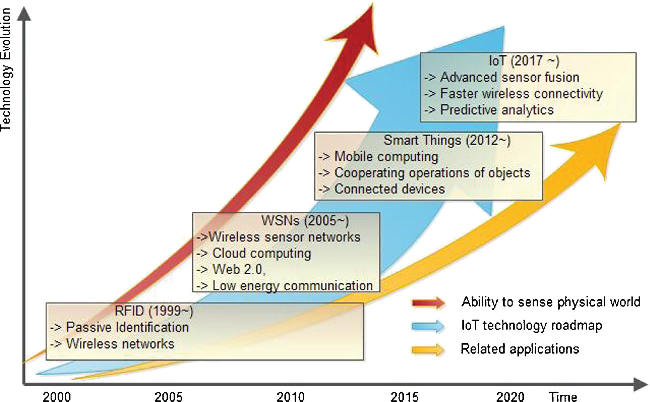
\includegraphics[scale=1.2]{Figures/IoTEvol}
	\caption{Evolución y aplicaciones de IoT\cite{li2015internet}.}
	\label{fig:IoTEvol}
\end{figure}

Con el incremento en la cantidad de servicios, también surgen otras necesidades. Algunas de ellas y quizá las más críticas en la arquitectura pensada para IoT, son la latencia de los datos y el rendimiento del sistema \cite{bonomi2012fog}. Por ello, se propone llevar algunos de los servicios de la nube más cerca del nivel al que se encuentran los datos así como emplear múltiples niveles, según las necesidades de las diferentes aplicaciones, como lo muestra la Figura \ref{fig:IoTDist}. En el caso del nivel \textit{Extremo} ó \textit{MIST}, se tienen niveles de procesamiento bajos; en este nivel, son los mismos nodos sensores y actuadores, los que toman decisiones operativas a un nivel muy bajo dadas las limitaciones en los procesadores que requieren para funcionar. A nivel de \textit{Borde} ó \textit{FOG}, se tiene mayor potencia de cálculo permitiendo realizar labores de almacenamiento, analítica, toma de decisiones, etc. Esto es posible, dado que en algunas aplicaciones, el dispositivo de borde, también conocido como Gateway, hace la labor de establecer un puente entre el extremo y la nube, contando con una radio potente y una conexión a Internet y alimentación eléctrica estables; es por estas necesidades que el gateway dentro de su concepción debe contar con hardware más potente que los demás dispositivos. Finalmente, sobre la última capa se encuentra la \textit{Nube} ó \textit{CLOUD}, el cual es el pilar más importante del Internet de las Cosas, ofreciendo múltiples servicios, con recursos prácticamente ilimitados en procesamiento, capaz de escalar dinámicamente conforme las necesidades lo requieran \cite{bonomi2014fog}.

\begin{figure}[!ht]
	\centering
		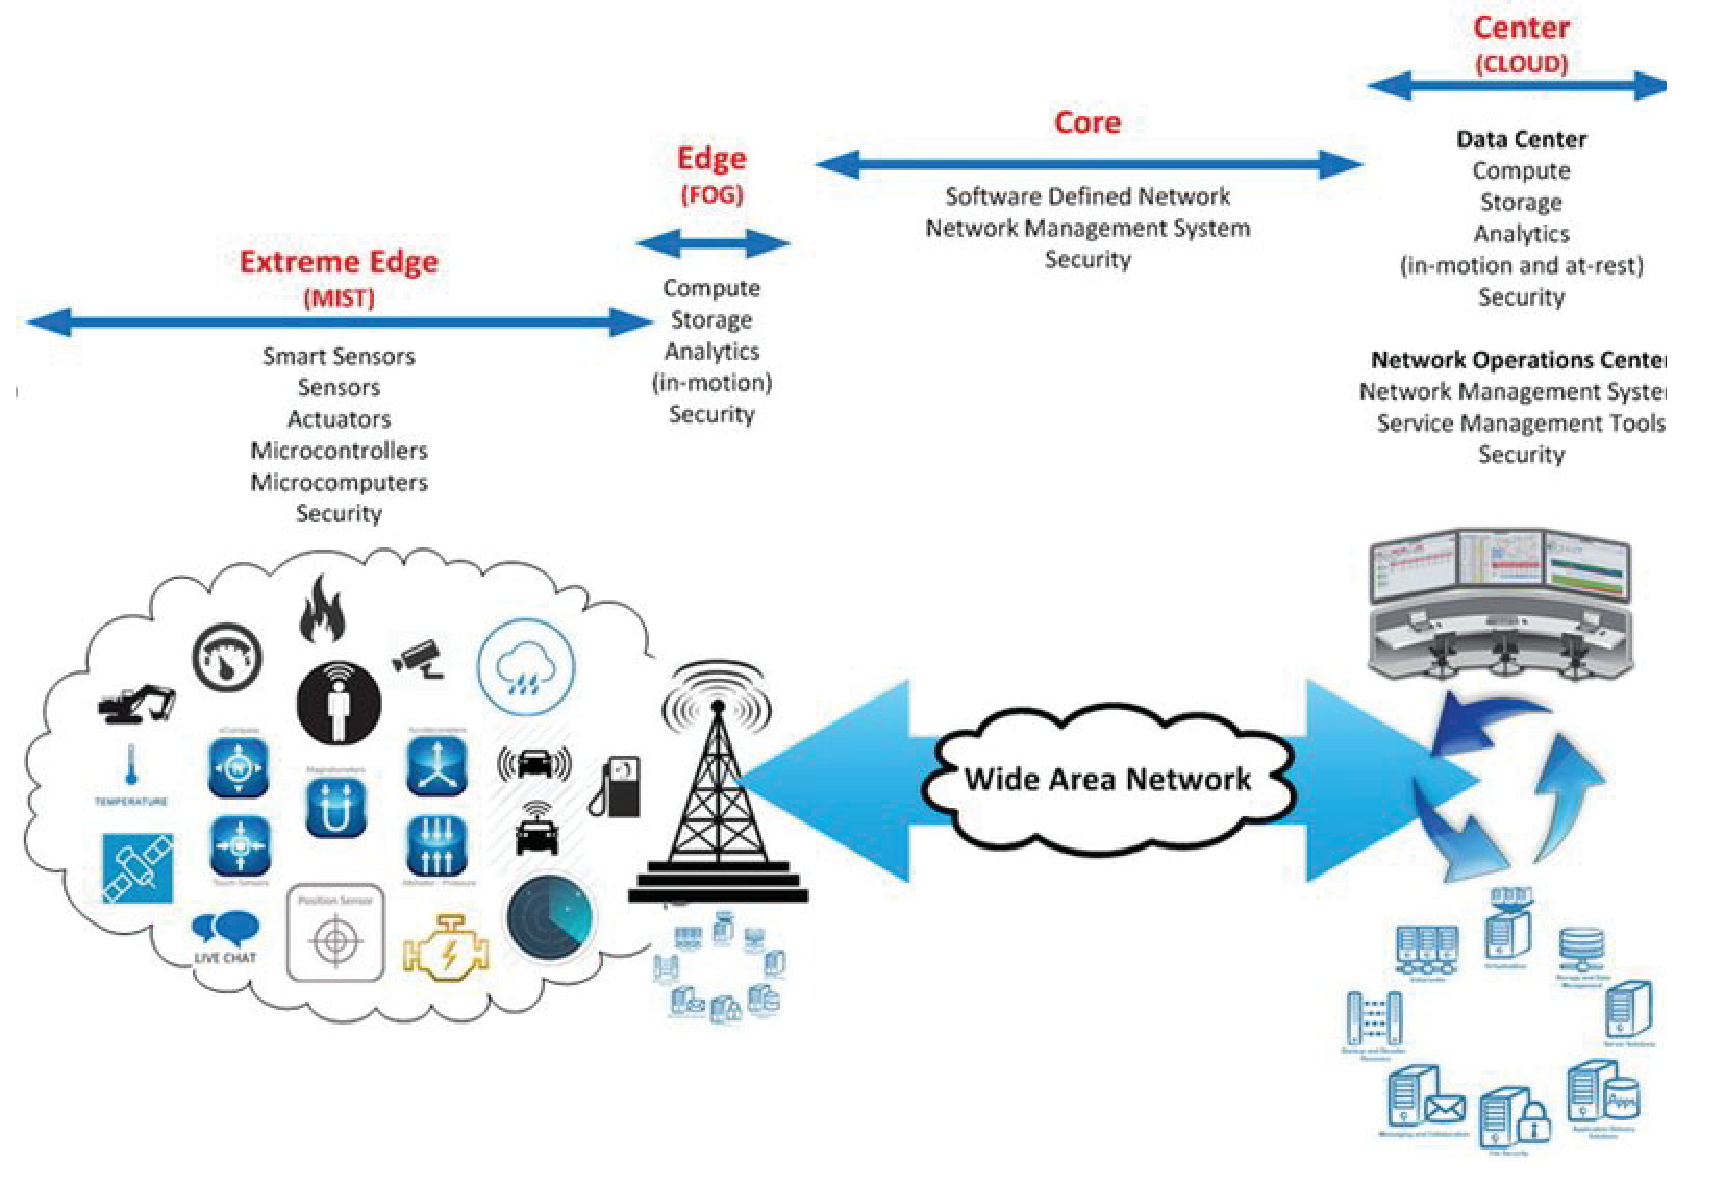
\includegraphics[scale=0.5]{Figures/IoTDist}
	\caption{Distribución del Internet de las Cosas (Operación)\cite{bonomi2012fog}.}
	\label{fig:IoTDist}
\end{figure}

Entonces, como se sugiere, la computación de borde está orientada a comunicación entre dispositivos, con una orientación a un almacenamiento y toma de decisiones eficientes. Esto implica directamente reducción en tiempo de procesamiento, almacenamiento, visualización y manejo de los datos como se muestra en la Figura \ref{fig:IoTFogGr}. 

Al final, la nube como el pilar fundamental, ofrece potencia de cálculo y por ende más servicios \cite{madsen2013reliability}, pero algunas de las aplicaciones únicamente requieren parte de estos servicios, que pueden ser resueltos en el borde por un gateway. Las aplicaciones que hacen uso de la computación de borde pueden ser de cualquier tipo; por ejemplo, encontramos modelos de programación para aplicaciones que requieran procesamiento de borde a gran escala \cite{hong2013mobile}, Gateways inteligentes capaces de enrutar de mejor manera los paquetes de red que tienen como destino la nube \cite{aazam2014fog}, modelos de \textit{centros de datos} para el procesamiento de datos efectivos en el borde \cite{aazam2015fog}, QoS distribuido dentro de la red de IoT \cite{cardellini2015distributed}. Como se ve, el concepto es ampliamente usado, pero el terreno sobre la aceleración por hardware sigue sin ser explorado, dadas las complicaciones que requiere su programación. Con sintetizadores de alto nivel apenas madurando, se espera avanzar hacia la creación de APIs ó middlewares que permitan a los desarrolladores incrementar la potencia de cálculo en el borde como lo sugieren las patentes \citep{subramanian2016dynamic,zhu2013improving}.

\begin{figure}[!ht]
	\centering
		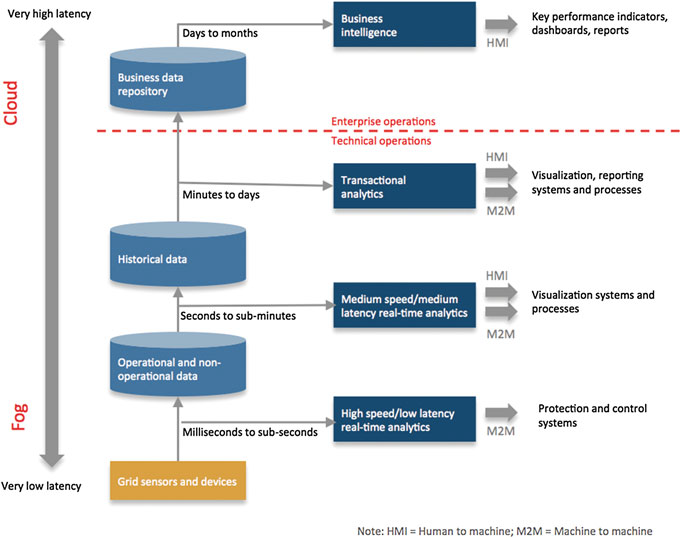
\includegraphics[scale=1.2]{Figures/IoTFogGr}
	\caption{Escalas de tiempos de servicios de la computación de borde vs la nube\cite{bonomi2014fog}.}
	\label{fig:IoTFogGr}
\end{figure}

\subsection{Síntesis de Alto Nivel \textit{HLS}}

La síntesis de alto nivel (\textit{HLS}, por las siglas en inglés de \textit{High-Level Sythesis}), le permite al desarrollador programar hardware usando lenguajes con altos niveles de abstracción como lo son C/C++, sin necesidad de hacer uso de lenguajes de descripción de hardware como VHDL o Verilog, cuyo desarrollo y simulación es lento y complejo comparado con el tiempo que toma desarrollar en un lenguaje de alto nivel. Actualmente, la tercera generación de compiladores de HLS ofrece a los desarrolladores ventajas significativas frente a las revisiones anteriores como lo son la optimización del proceso de síntesis de hardware, la estandarización del uso de C, C++ y System C como lenguajes de entrada al software de síntesis y la posibilidad de adicionar directivas de optimización sin realizar modificaciones al código fuente, co-simulación entre los diferentes lenguajes de entrada y el RTL objetivo, entre otras \cite{HLStory}.

Las bondades de HLS frente a los paradigmas de programación de hardware tradicionales son muchas como se mencionó anteriormente. Una de ellas y quizá de las más importantes, es la aplicación de optimizaciones de hardware que, según el contexto, puede incrementar el rendimiento de un circuito, modificando la cantidad de hardware dedicado al procesamiento de cada tarea \cite{HLSeffect,canis2013legup}. 

Por otra parte, HLS provee al desarrollador la opción de crear hardware reconFigurable de forma dinámica; esto es conocido como reconFiguración parcial o \textit{PR} por sus siglas en inglés. La aplicación de la reconFiguración parcial le permite al desarrollador integrar múltiples módulos de hardware con diferentes algoritmos que pueden ser instanciados sobre la superficie de la FPGA de forma dinámica \citep{kao2005benefits,wehner2014using,owens2013design}, con el objetivo de tener en un único dispositivo, múltiples funciones sin la necesidad de reprogramar la FPGA completamente.

Entre los proyectos orientados a usar netamente HLS como medio de prototipado e implementación de sistemas hardware, se pueden encontrar soluciones desde, optimizar procesos de kernel de un S.O., pasando por acceder y modificar bases de datos de forma concurrente usando paralelismo y finalizando con la fusión de datos  \citep{liu2013soft,monson2015using,navarro2013high,malazgirt2015high,choi2013software,alias2013optimizing,zhao2015area,liu2015moving}.

\subsection{Computación Consciente del Contexto}

Cuando se habla de grandes cantidades de datos recolectada por miles de sensores dentro de un esquema de IoT, se pone sobre la mesa una pregunta: ¿Cómo interpretar los datos?. Es importante notar que por más información que se tenga disponible, si no se analiza, interpreta y entiende dentro de un contexto dado, esta información no tiene valor alguno.

La computación consciente del contexto, vista desde una perspectiva de IoT, propone una forma de mediar con la información desde diferentes flancos. Actualmente hablamos de la implementación de soluciones middleware capaces de añadir recursos que se encarguen de abstraer, fusionar y comprimir los datos, además de añadir servicios como QoS, paradigmas de programación, adaptabilidad, escalabilidad, recursos de hardware y lo más importante, seguridad de los datos \citep{molla2006survey}.

\begin{figure}[!ht]
	\centering
		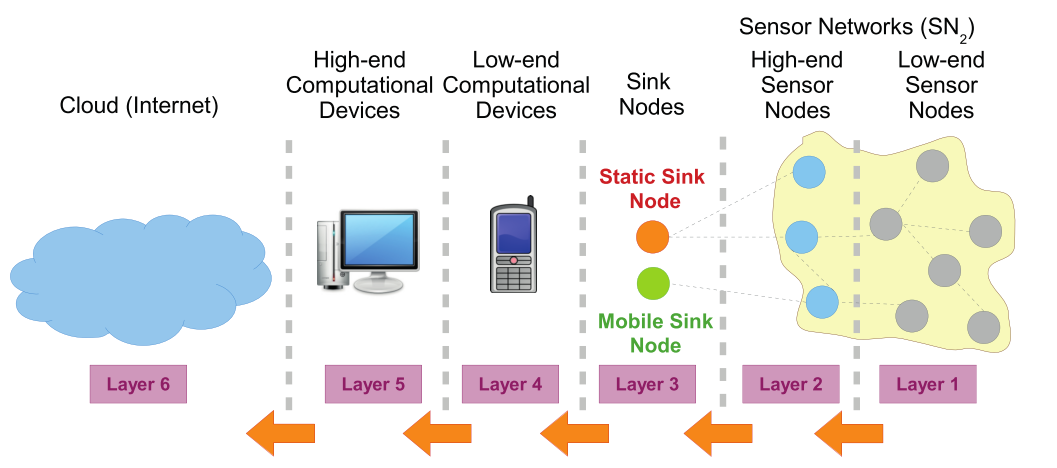
\includegraphics[scale=0.85]{Figures/Structure_of_a_sensor_network}
	\caption{Red de sensores estructurada por capas \citep{perera2014context}.}
	\label{fig:IoTWSN2Cloud}
\end{figure}

La Figura \ref{fig:IoTWSN2Cloud} ofrece una vista general de la forma como se distribuye una red de sensores por capas, desde los elementos más básicos hasta los más complejos. En las primeras tres capas se observa el flujo de datos que va desde los dispositivos menos potentes hasta los más potentes en la capa 3, que muchas veces hacen las veces de enrutadores de borde de red. En las capas 4 y 5 se tienen dispositivos computacionalmente mucho más potentes; estos son conocidos como Gateways, capaces de llevar la información del campo hacia la nube. Finalmente, se tiene la Nube en Internet, donde la información capturada puede ser transformada y procesada para su análisis. Cada una de las capas cumple un rol específico en el que la eficiencia es la clave\citep{sho2008ttcg}. Nótese que el procesamiento se podría realizar entre las dos primeras capas reduciendo considerablemente el costo de las comunicaciones; sin embargo, las limitaciones en capacidad de cómputo y energéticas impedirían realizar un análisis detallado de la información recolectada por la red.

En función de esta necesidad, los investigadores definieron siete grandes características que permiten enmarcar una solución para el IoT dentro del contexto de la computación consciente del contexto que, necesariamente, dadas las condiciones, deben ser realizadas entre las capas cuatro a seis \citep{sundmaeker2010vision}. Estas son: inteligencia, arquitectura, sistemas complejos, magnitud, tiempo, espacio y ``Todo como un Servicio'' o ``All as a Service''. Algunas de estas cobran particular interés, como inteligencia, pues determina que para usar la información recolectada por diferentes fuentes en crudo se debe transformar para lograr lo que se denomina \textit{información de alto nivel}, que lo que quiere decir es que esta información nueva enriquecida y puesta en un contexto, pueda ser usada como insumo para otro tipo de operaciones. Otra de las características que cobra particular interés es la de tiempo, pues dados los altos volúmenes de transacciones de datos se hacen necesarios mecanismos que permitan operar en tiempo real, siendo una restricción importante cuando se modela una solución de este tipo. 
%tek
%
% > siete características versus seis enunciadas
%
% > inteligencia, arquitectura, sistemas complejos, magnitud, tiempo, espacio

A partir de este punto, se introduce el concepto \textit{``Principios Administrativos de Diseño Consciente del Contexto"}, que básicamente se define como, los requerimientos para la aplicación de un middleware consciente del contexto de operación, que se encuentre en capacidad de analizar, transformar e interactuar con el medio para darle sentido a la información \citep{martin2010automatic,ramparany2007open,bernardos2008data}. Uno de los requerimientos más tangibles es el llamado \textit{optimización de recursos}, el cual implica que, cualquier mejora en los recursos de procesamiento, por más pequeña que sea, tendrá un gran impacto en el procesamiento dados los altos volúmenes de información que el IoT puede llegar a procesar.

Finalmente, tenemos la definición estricta de Schilit \citep{schilit1994context} en la que, una aplicación consciente del contexto, no es más que un dispositivo que cumple unas reglas básicas según la operación que realiza, desde la toma simple de decisiones basado en eventos hasta la resolución de los mismos usando ventanas de oportunidad en las que las condiciones del evento establecen las fronteras. 

\subsection{Monitoreo y predicción de inundaciones}

Las inundaciones son uno de los fenómenos naturales más comunes y destructivos que puede enfrentar la humanidad; esto debido a los altos niveles de precipitación, el cambio climático, y represamientos ya sean naturales o artificiales. Existen diferentes atributos que pueden favorecer o prevenir una inundación; estos son mostrados en la Tabla \ref{tab:floodAtributes}. En ella, se dispone información, que según estudios \citep{floodAtributes}, son los factores determinantes de mayor ocurrencia en lugares donde ocurren inundaciones.

\begin{table}[ht!]
\centering
\resizebox{\textwidth}{!}{%
\begin{tabular}{@{}ccccccc@{}}
\toprule
Categoría & Atributos & Aumento del orden de ocurrencia -\textgreater{} &  &  &  &  \\ \midrule
\begin{tabular}[c]{@{}c@{}}Causantes de\\ Inundación\end{tabular} & \begin{tabular}[c]{@{}c@{}}Precipitación Media\\ Velocidad de Captación\end{tabular} & \begin{tabular}[c]{@{}c@{}}Muy poca\\ Constante\end{tabular} & \begin{tabular}[c]{@{}c@{}}Poca\\ Poco flujo\end{tabular} & \begin{tabular}[c]{@{}c@{}}Moderada\\ Flujo moderado\end{tabular} & \begin{tabular}[c]{@{}c@{}}Alta\\ Flujo Alto\end{tabular} & \begin{tabular}[c]{@{}c@{}}Extrema\\ Flujo Extremo\end{tabular} \\
\begin{tabular}[c]{@{}c@{}}Prevención de\\ Inundación\end{tabular} & \begin{tabular}[c]{@{}c@{}}Orden del flujo\\ Densidad del bosque por área\\ Estación actual\\ Sistemas de drenaje\\ Tipo de suelo\end{tabular} & \begin{tabular}[c]{@{}c@{}}1\\ Bosque Denso \textgreater 1000\\ Invierno\\ El mejor\\ Arenoso\end{tabular} & \begin{tabular}[c]{@{}c@{}}2\\ Bosque Espeso 800-1000\\ Primavera\\ Bueno\\ Granular\end{tabular} & \begin{tabular}[c]{@{}c@{}}3\\ Bosque Pequeño 500-800\\ Otoño\\ Promedio\\ Orgánico\end{tabular} & \begin{tabular}[c]{@{}c@{}}4\\ Tierra de Cultivo 100-500\\ Verano\\ Malo\\ Arcilla\end{tabular} & \begin{tabular}[c]{@{}c@{}}5\\ Tierra Estéril \textless 100\\ Monzón\\ La peor\\ Compacto\end{tabular} \\ \bottomrule
\end{tabular}%
}
\caption{Atributos que causan o previenen inundaciones}
\label{tab:floodAtributes}
\end{table}

%Teniendo esta información a mano es posible determinar qué lugares son propensos a presentar inundaciones; históricamente se ha determinado que China es uno de los países más afectados por las inundaciones\citep{ChinaFloods}, convirtiéndolo en uno de los focos de atención para la implementación de soluciones que determinen con antelación un desastre. En Colombia no estamos lejos de perder vidas humanas a causa de las inundaciones, donde anualmente se pierden cientos de vidas y muchas otras personas pierden sus casas a causa de deslizamientos y ruptura de las barreras que protegen a los habitantes.

Las investigaciones alrededor del tema van desde monitorear las precipitaciones remotamente desde satélite\cite{remoteSatellite,advancedForecast} con resultados observables que muestran altos niveles de incertidumbre, pasando por modelos fuzzy que se ven altamente beneficiados por su habilidad de crear relaciones unificadas alrededor de la información hidrológica, hasta el uso de redes neuronales para determinar los niveles del agua a lo largo de múltiples estaciones meteorológicas donde la correlación entre los datos es importante y determinante para realizar las predicciones\cite{Nguyen2014,floodfc1,floodfc2,floodfc3,floodfc4}.

Según \citep{floodAtributes}, un sistema de monitoreo eficiente debería tener múltiples factores ejecutados en secuencia.
\begin{itemize}
\item Recopilación correcta de los datos.
\item Análisis efectivo de la información.
\item Notificaciones tempranas de los resultados.
\end{itemize}

Para ello se proponen diferentes soluciones; una de ellas, es una solución multicapa en la que se realicen estas operaciones, siendo la capa más baja la capa IoT donde se adquieran los datos, una capa de computación de borde, una capa de análisis de datos y finalmente, la capa más alta conocida como la capa de presentación. Cada una de estas capas realiza una actividad específica, siendo la capa de computación de borde la usada para reducir la latencia de toda la solución.

La predicción oportuna y efectiva de inundaciones depende de varios factores; algunos de ellos están clasificados en la Tabla \ref{tab:floodAtributes} y hay otros, como la ubicación estratégica de los nodos de medición, siendo este el factor que más puede influenciar en la predicción, pues es necesario que la información no se vea solapada y que el modelo se encuentre correctamente establecido para la zona. Por ejemplo, en \citep{floodAtributes}, se propone una distribución hexagonal de los diferentes nodos; en \citep{floodfc3} se propone distribuir los sensores a lo largo de la cuenca del río a analizar. Por otro lado, la precisión de la predicción se ve afectada por la configuración y tipo de modelo usado, como por ejemplo, modelos hidrológicos e hidrodinámicos que permiten tener simulaciones bastante precisas \citep{merkuryeva2015advanced,ANN3} que son complejos y requieren análisis, medidas de los ríos y conocimientos específicos para que sean factibles. Finalmente, están los basados en redes neuronales, que son adaptables a la gran cantidad de información y variables que se requieren para realizar una predicción sin conocer específicamente la relación entre las entradas y las salidas del sistema; lo que se busca con estos modelos es tener una predicción en línea, con bajas latencias y sin necesidad de realizar un post-procesamiento de los datos en servidores lejos de la zona de interés. Estas aproximaciones han sido usadas para estimar el nivel de los ríos usando hardware embebido \cite{ANN1,ANN2,ANN3,ANN4,ANN5,ANN6,ANN7}.

\section{Síntesis de Alto Nivel}

\subsection{Herramientas de Síntesis}

Dentro de las herramientas de síntesis de alto nivel es posible encontrar una amplia gama de desarrollos; entre ellos, los más modernos son:

\begin{table}[!ht]
\centering
\begin{tabular}{|l|c|c|c|}
\hline
\multicolumn{1}{|c|}{\textbf{Compilador}} & \textbf{Desarrollador} & \textbf{Lenguaje} & \textbf{Salida} \\ \hline
A++ & Altera & C/C++ & \begin{tabular}[c]{@{}c@{}}VHDL\\ Verilog\end{tabular} \\ \hline
Vivado HLS & Xilinx & \begin{tabular}[c]{@{}c@{}}C/C++\\ System C\end{tabular} & \begin{tabular}[c]{@{}c@{}}VHDL\\ Verilog\end{tabular} \\ \hline
Stratus & Cadence & \begin{tabular}[c]{@{}c@{}}C/C++\\ System C\end{tabular} & RTL \\ \hline
Hastlayer & \begin{tabular}[c]{@{}c@{}}Lombiq\\ Technology\end{tabular} & \begin{tabular}[c]{@{}c@{}}.NET\\ C/C++/F\#\end{tabular} & VHDL \\ \hline
LegUp HLS & \begin{tabular}[c]{@{}c@{}}LegUp\\ Computing\end{tabular} & C & Verilog \\ \hline
Kiwi & \begin{tabular}[c]{@{}c@{}}Universidad de\\ Cambridge\end{tabular} & C\# & Verilog \\ \hline
HercuLeS & \begin{tabular}[c]{@{}c@{}}Ajax\\ Compilers\end{tabular} & C/NAC & VHDL \\ \hline
\begin{tabular}[c]{@{}l@{}}Matlab\\ HDL Coder\end{tabular} & Matlab/Xilinx & \begin{tabular}[c]{@{}c@{}}Matlab\\ Script\end{tabular} & VHDL \\ \hline
\end{tabular}
\caption{Sintetizadores de alto nivel más comunes}
\label{tab:sintetizadores}
\end{table}

Entre los desarrolladores de la Tabla \ref{tab:sintetizadores}, encontramos a Altera y Xilinx, desarrollares de chips FPGA, así como importantes desarrolladores de software como Mathworks con su software de síntesis HDL Coder.

\subsubsection{Esquema General de Síntesis}

En su núcleo, los sintetizadores de alto nivel siguen un mismo esquema de compilación, el cual sigue los siguientes pasos:

\begin{itemize}
\item Procesamiento léxico
\item Optimización del algoritmo
\item Análisis de control y flujo de datos
\item Procesamiento de bibliotecas
\item Asignación de recursos
\item Agendamiento
\item Unión de funciones
\item Unión de registros
\item Procesamiento de salidas
\item Reducción de entradas
\end{itemize}

La diferencia entre cada uno de los sintetizadores radica principalmente en la cantidad de lenguajes de entrada, la cantidad de optimizaciones y la calidad de las mismas aplicadas al hardware final.

\subsubsection{Optimizaciones de Hardware}

Cada sintetizador puede ofrecer una gama diferente de optimizaciones; estas pueden ser aplicadas al código fuente usando una directiva del lenguaje, como por ejemplo,\textbf{pragma} en el caso de C y sus derivados. A través de ella, se le indican directamente al compilador,  parámetros de entrada como conFiguraciones dependiendo del tipo de optimización a aplicar.

Para el caso particular de Vivado HLS, la Tabla \ref{tab:HLS} muestra las directivas de optimización y una breve descripción del propósito.

\begin{table}[H]
\centering
\resizebox{\linewidth}{!}{%
\begin{tabular}{|l|l|}
\hline
\textbf{Directiva} & \textbf{Descripción}                                                                                                                                                                                                                                                                      \\ \hline
ARRAY\_MAP         & \begin{tabular}[c]{@{}l@{}}Permite combinar diferentes arreglos de tamaño reducido en uno solo de \\ gran tamaño con el objetivo de reducir la cantidad de BRAM requerida \\ en la solución.\end{tabular}                                                                           \\ \hline
ARRAY\_PARTITION   & \begin{tabular}[c]{@{}l@{}}Permite transformar un arreglo de gran tamaño en sub arreglos de menor \\ tamaño buscando reducir las contenciones en las memorias BRAM Dual\\  Port.\end{tabular}                                                     \\ \hline
ARRAY\_RESHAPE     & \begin{tabular}[c]{@{}l@{}}Permite transformar un arreglo con muchos elementos de tamaño reducido \\ a uno de menor cantidad de elementos individuales pero con mayor ancho \\ de datos. Esta directiva es útil para reducir la cantidad de accesos a\\   memoria RAM.\end{tabular} \\ \hline
DATA\_PACK         & \begin{tabular}[c]{@{}l@{}}Empaqueta los campos de una estructura en un solo arreglo con mayor\\   ancho de datos.\end{tabular}                                                                                                                                                        \\ \hline
DATAFLOW           & \begin{tabular}[c]{@{}l@{}}Habilita un pipeline a nivel de tareas, permitiendo que funciones y bucles \\ operen de forma concurrente.\end{tabular}                                                                                                                               \\ \hline
LATENCY            & \begin{tabular}[c]{@{}l@{}}Permite especificar la latencia del circuito a implementar; esta puede ser \\ tanto mínima como máxima.\end{tabular}                                                                                                                       \\ \hline
LOOP\_FLATTEN      & \begin{tabular}[c]{@{}l@{}}Permite combinar bucles anidados en un solo bucle; esta directiva mejora \\ considerablemente la latencia del circuito únicamente si los bucles son \\ considerados perfectos.\end{tabular}                                                              \\ \hline
LOOP\_MERGE        & \begin{tabular}[c]{@{}l@{}}Permite combinar bucles consecutivos en uno solo mejorando la latencia \\ del circuito.\end{tabular}                                                                                                                                                      \\ \hline
PIPELINE           & \begin{tabular}[c]{@{}l@{}}Permite reducir el intervalo de iniciación, permitiendo que las tareas \\ a nivel de función o bucle se ejecuten concurrentemente.\end{tabular}                                                                                        \\ \hline
UNROLL             & \begin{tabular}[c]{@{}l@{}}Usada para desglosar un bucle \texttt{for} en múltiples operaciones independien-\\tes; esta directiva busca incrementar la productividad haciendo uso del \\ paralelismo.\end{tabular}                                                                            \\ \hline
CLOCK              & Permite cambiar el dominio de tiempo de una función.                                                                                                                                                                                                                                  \\ \hline
INLINE             & \begin{tabular}[c]{@{}l@{}}Usada para crear optimizaciones lógicas entre funciones, reduciendo así \\ la latencia y la sobrecarga de llamados a la función.\end{tabular}                                                                                                     \\ \hline
\end{tabular}
}
\caption{Directivas disponibles en Vivado HLS \citep{HLS2015}}
\label{tab:HLS}
\end{table}

La directiva ARRAY\_MAP permite realizar el mapeo de los arreglos de dos formas diferentes que pueden beneficiar de diferentes formas el circuito, los cuales son el mapeo horizontal y el mapeo vertical.

\textbf{Mapeo Horizontal:} El resultante de aplicar la directiva ARRAY\_MAP con la opción de mapeo horizontal implica la creación de un nuevo arreglo con los diferentes arreglos concatenados uno tras otro. 

En la Figura \ref{fig:HLS7}, se aprecia la aplicación de la directiva ARRAY\_MAP con Mapeo Horizontal. Este tipo de implementaciones permite reducir la cantidad de BRAM presente en el circuito.

\begin{figure}[H]
	\centering
		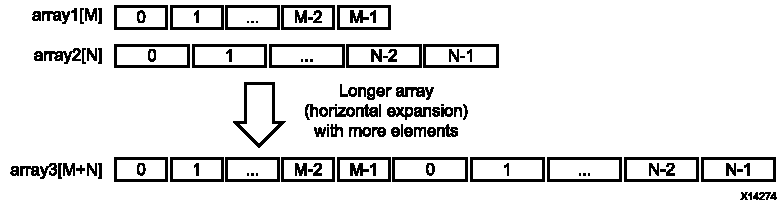
\includegraphics[scale=0.8]{./Figures/HLS7.pdf}
	\caption{Directiva ARRAY\_MAP en modo horizontal \citep{HLS2015}}
	\label{fig:HLS7}
\end{figure}

En la Figura \ref{fig:HLS10} se ve la aplicación en RAM de la directiva. Se puede notar que se toma una BRAM del tamaño de datos más ancho. Los bits sobrantes son descartados.

\begin{figure}[H]
	\centering
		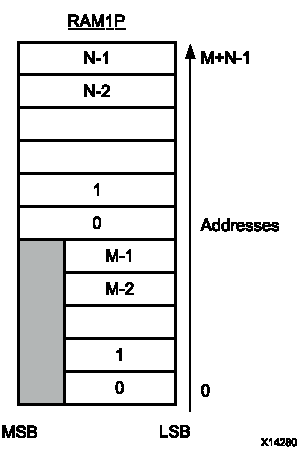
\includegraphics[scale=0.8]{./Figures/HLS10.pdf}
	\caption{Distribución en RAM del Mapeo Horizontal \citep{HLS2015}}
	\label{fig:HLS10}
\end{figure}

Implementaciones de este tipo traen complicaciones que pueden afectar de manera directa el rendimiento del circuito, pues dadas las grandes dimensiones y la limitada cantidad de puertos, se pueden presentar contenciones que darán lugar al efecto cuello de botella, donde la unidad de control deberá agendar los accesos a la RAM de tal forma que se extraigan los datos según la cantidad de peticiones.

\textbf{Mapeo Vertical:} Esta implementación consiste en la creación de un nuevo arreglo donde se concatenan los datos uno junto a otro; esto implica la creación de un arreglo de tamaño igual a la cantidad de datos individuales pero con un ancho de bits igual a la suma de los anchos de los arreglos a unir.

En la Figura \ref{fig:HLS8} se puede observar una representación del Mapeo Vertical; en este caso se han tomado dos arreglos de ancho e índices diferentes y se han concatenado elemento a elemento para formar un arreglo de mapeo vertical.

\begin{figure}[H]
	\centering
		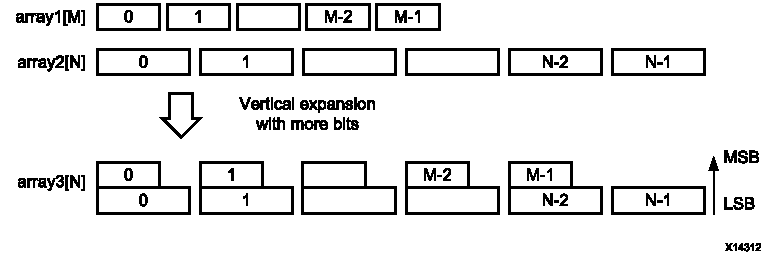
\includegraphics[scale=0.8]{./Figures/HLS8.pdf}
	\caption{Directiva ARRAY\_MAP en modo vertical \citep{HLS2015}}
	\label{fig:HLS8}
\end{figure}

El orden de concatenado se da a elección del diseñador, el cual le indica al sintetizador cuál subarreglo deberá ocupar la parte baja del elemento del arreglo y cuál la parte alta.

En la Figura \ref{fig:HLS11}, se aprecia cómo sería la distribución en la memoria RAM del mapeo vertical. En este caso, uno de los arreglos tiene mayor número de elementos que el otro y los bits restantes son puestos a tierra por el sintetizador.

\begin{figure}[H]
	\centering
		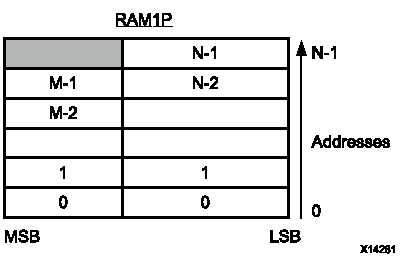
\includegraphics[scale=0.8]{./Figures/HLS11.pdf}
	\caption{Distribución en RAM del Mapeo Vertical  \citep{HLS2015}}
	\label{fig:HLS11}
\end{figure}

Otra de las directivas de Vivado HLS es la llamada ARRAY\_PARTITION. Esta directiva permite al programador incrementar el rendimiento del circuito cuando este se ve envuelto en un cuello de botella debido a las contenciones; esto se debe al número limitado de puertos con los que cuentan las memorias Block RAM de la FPGA y que el sistema intenta acceder simultáneamente a diferentes entradas que se encuentran en la misma memoria BRAM, como ocurre al aplicar la directiva PIPELINE.

\begin{figure}[H]
	\centering
		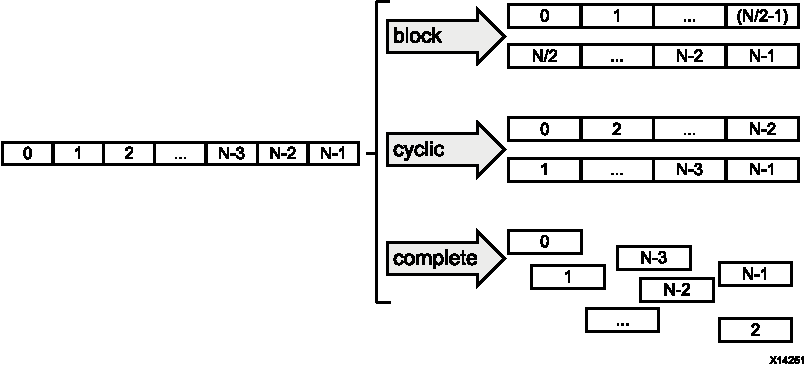
\includegraphics[scale=0.8]{./Figures/HLS5.pdf}
	\caption{Modos de operación de la directiva ARRAY\_PARTITION \citep{HLS2015}}
	\label{fig:HLS5}
\end{figure}

En la Figura \ref{fig:HLS5} se pueden observar los modos de operación de la directiva ARRAY\_PAR-\\TITION, los cuales se detallarán a continuación.

\begin{itemize}
\item \textbf{Bloque:} En este caso, el arreglo que se desea particionar será dividido en un número de acuerdo a un factor especificado por el diseñador y las necesidades del hardware.

\item \textbf{Cíclico:} Este modo permite particionar el arreglo de modo que se intercalen los índices del arreglo. En este modo también es posible adicionar un factor de partición.

\item \textbf{Completo:} En modo completo el sintetizador transformará el arreglo en registros individuales permitiendo acceder a cada elemento de forma individual; esto implica un aumento significativo de los recursos de hardware usados para cumplir el funcionamiento del circuito.
\end{itemize}

Continuando con el detalle de las directivas encontradas en Vivado HLS encontramos la directiva ARRAY\_RESHAPE, la cual es una combinación de  dos directivas anteriormente mencionadas: ARRAY\_MAP en modo vertical y ARRAY\_PARTITION. Esta directiva permite reducir el número de BRAM a usarse en la solución final y a su vez mantiene el beneficio de particionar los arreglos, cual es el acceso paralelo a los datos contenidos en la memoria.

La Figura \ref{fig:HLS12} nos muestra un ejemplo claro del funcionamiento de la directiva.

\begin{figure}[H]
	\centering
		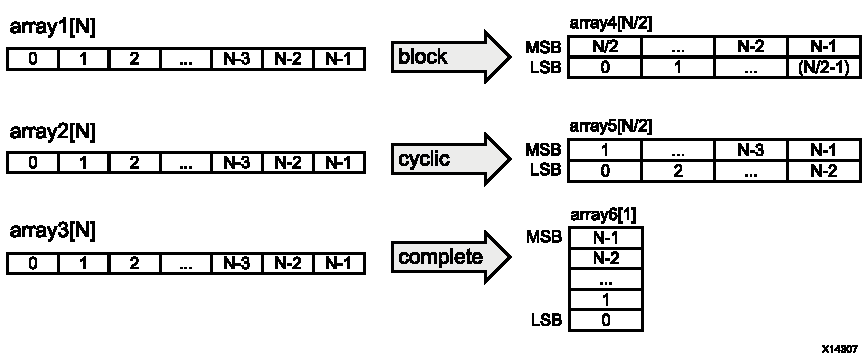
\includegraphics[scale=0.8]{./Figures/HLS12.pdf}
	\caption{Modos de operación de la Directiva ARRAY\_RESHAPE \citep{HLS2015}}
	\label{fig:HLS12}
\end{figure}

En este caso particular se han elegido tres arreglos diferentes de tamaño N; en ellos se ha elegido una partición en factor de dos para los modos BLOQUE y CICLICO. Como se mencionó anteriormente, cada uno de los elementos del índice se concatena usando el modo vertical del ARRAY\_MAP. En el caso del modo COMPLETO se concatena cada uno de los elementos para formar un solo elemento de ancho N, siendo el bit menos significativo el primer elemento del índice original y el bit más significativo el último bit del último elemento del índice original.

Dentro de las posibilidades de desarrollo usando síntesis de alto nivel con lenguajes como C/C++, surge la necesidad de adicionar el tipo de dato STRUCT o estructura; esto permite crear un tipo de dato el cual puede combinar diferentes tipos de datos en su interior. Estos datos no son más que referencias a posiciones de memoria, las cuales usan desplazamientos relativos (offsets) según el tipo de dato a acceder.

Sin embargo, a nivel de hardware, el acceso a los elementos individuales puede ser complejo dada la cantidad de elementos que la estructura puede contener. Por omisión, el sintetizador asume que cada arreglo dentro una estructura es una BRAM independiente, es por esto que se debe crear una lógica de control independiente para cada una de estas memorias.

En la Figura \ref{fig:HLS13} se observa el funcionamiento de la directiva DATA\_PACK, la cual permite optimizar el acceso a la estructura.

\begin{figure}[H]
	\centering
		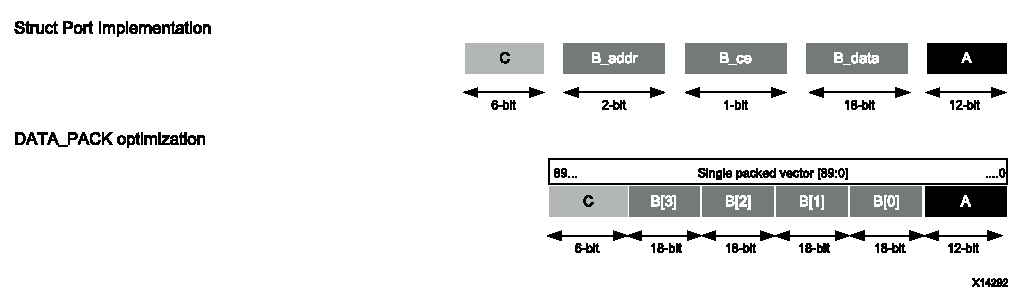
\includegraphics[scale=0.8]{./Figures/HLS13.pdf}
	\caption{Funcionamiento de la Directiva DATA PACK \citep{HLS2015}}
	\label{fig:HLS13}
\end{figure}

En este caso particular, el elemento A es un elemento individual de tipo int12, el elemento B es un arreglo de 4 elementos de tamaño int18 y finalmente el elemento C, es un elemento individual de tamaño int6. Como se infiere de la parte superior de la imagen, la implementación de la estructura implica que el sintetizador haga uso de dos LUT RAM para ocupar los elementos A y C y una BRAM para ocupar el elemento B con su respectiva lógica de control. Posterior a la optimización, es posible tener una sola BRAM conteniendo todos los elementos de la estructura; de esta forma, se puede reducir el hardware necesario para el funcionamiento del circuito reduciendo así la latencia del mismo.

Dentro de las posibilidades de realizar operaciones concurrentes con Vivado HLS podemos encontrar la directiva DATAFLOW. Esta directiva transforma el código de tal forma que es posible tener un paralelismo a nivel de tareas o procesos dentro del mismo algoritmo haciendo uso de pipeline.

En la Figura \ref{fig:HLS14} podemos apreciar el esquema de un circuito resuelto de manera secuencial usando funciones.

\begin{figure}[H]
  \centering
    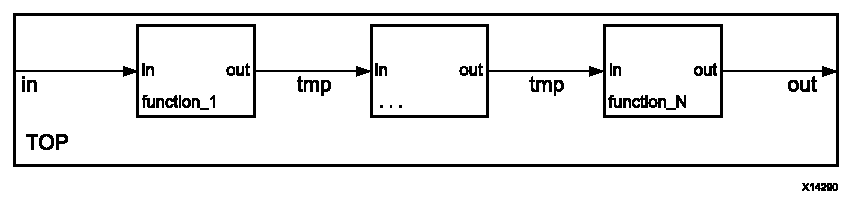
\includegraphics[scale=0.8]{./Figures/HLS14.pdf}
  \caption{Sistema secuencial  \citep{HLS2015}}
  \label{fig:HLS14}
\end{figure}

De esta forma es usual atacar la mayor cantidad de problemas si tienen una baja complejidad y cuentan con dependencias a nivel de datos como la variable \texttt{tmp} que se pasan las funciones en el módulo \texttt{TOP}.

Como se mencionó antes, la directiva DATAFLOW es capaz de transformar el código de tal forma que se crean canales de comunicación entre las diferentes funciones dividiendo las tareas entre procesos. Esto se puede observar en la Figura \ref{fig:HLS15}, donde la creación de los canales asegura que no se deba esperar a que termine la operación para continuar con las demás tareas.

\begin{figure}[H]
  \centering
    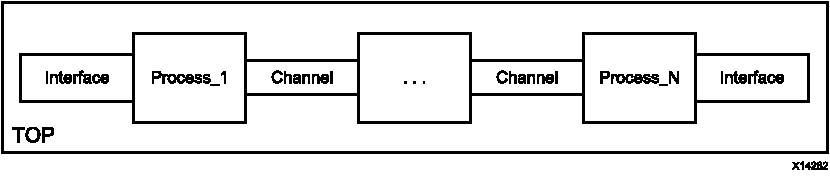
\includegraphics[scale=0.8]{./Figures/HLS15.pdf}
  \caption{Sistema concurrente a nivel de tareas \citep{HLS2015}}
  \label{fig:HLS15}
\end{figure}

En la Figura \ref{fig:HLS16} podemos ver un ejemplo claro del funcionamiento de la directiva DATAFLOW.

\begin{figure}[H]
  \centering
    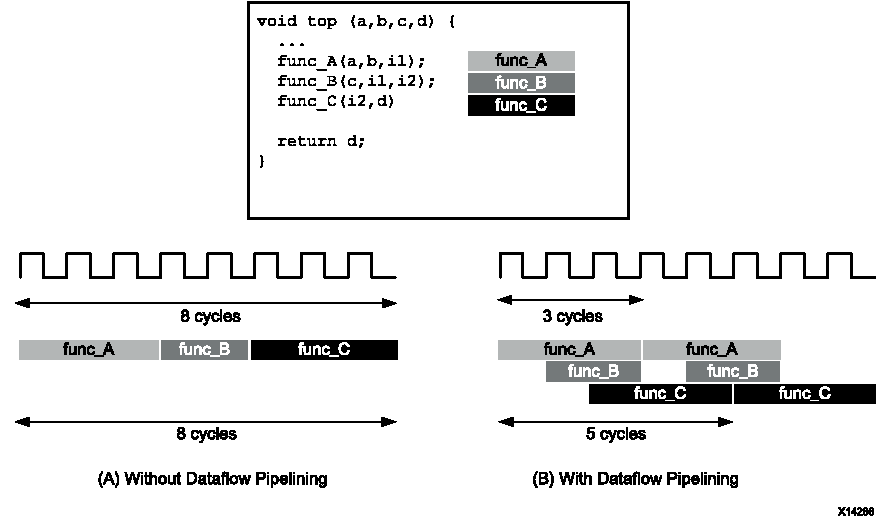
\includegraphics[scale=0.8]{./Figures/HLS16.pdf}
  \caption{Funcionamento de la directiva DATAFLOW \citep{HLS2015}}
  \label{fig:HLS16}
\end{figure}

En el lado (A) es posible ver cómo la operación tarda hasta 8 ciclos desde que se inicia la operación con \texttt{func\_A} y la salida del sistema \texttt{d} es escrita en memoria por \texttt{func\_C}. Usando la directiva DATAFLOW es posible aumentar la tasa a la que se obtienen resultados dada la operación en paralelo de las funciones usadas para calcular los resultados; en este caso, en el lado (B) vemos cómo el sistema es capaz de aceptar una nueva entrada al sistema cada 3 ciclos de reloj a diferencia de cada 8 ciclos sin la optimización y además, es posible obtener resultados cada 5 ciclos de reloj desde que ingresa un dato nuevo al circuito.

La directiva DATAFLOW requiere de condiciones específicas para garantizar la síntesis del circuito dentro de las cuales se deben cumplir los siguientes requerimientos:

\begin{itemize}
\item El sistema no debe tener ningún tipo de dependencia de datos.
\item Las funciones no deben tener retroalimentación.
\item Todas las funciones se deben ejecutar sin condiciones (\texttt{if}/\texttt{else}).
\item Los límites de los bucles deben ser fijos.
\item El sistema no puede tener paradas condicionales.
\end{itemize}

Vivado HLS es capaz de controlar la latencia de un bucle o una porción de código como tal; para esto es necesario usar la directiva LATENCY. Esta directiva restringe al sintetizador a alcanzar los valores de latencia indicados por el diseñador; en caso de no poder satisfacerlos, dadas las restricciones de hardware y propagación de los datos, el sintetizador tratará de alcanzar el nivel más bajo posible al indicado en el parámetro de la directiva.

Continuando con las mejoras en latencia de los circuitos usando Vivado HLS, podemos encontrar directivas como LOOP\_FLATTEN; esta directiva permite aplanar bucles anidados permitiendo reducir la latencia del bucle completo pues se elimina la lógica de control entre bucles.

La directiva LOOP\_FLATTEN requiere que el bucle a aplanar sea Perfecto o Semi-Perfecto; en el caso de ser un bucle imperfecto la directiva no será aplicada.

\begin{itemize}

\item \textbf{Bucle Anidado Perfecto:} Un bucle anidado perfecto es aquel en el cual no hay lógica entre bucles y únicamente el bucle más interior contiene lógica; además, los límites de los bucles son constantes.

\item \textbf{Bucle Anidado Semi-Perfecto:} Igual que el Bucle Anidado Perfecto, excepto porque los límites del bucle más externo pueden ser variables.

\end{itemize}

Además de la directiva de LOOP\_FLATTEN podemos encontrar la directiva LOOP \_MERGE. Esta directiva permite combinar bucles consecutivos no anidados e implica una mejora en la latencia general del sistema al reducir algunos ciclos de reloj entre la transición de bucles; este tiempo muerto se debe a que el circuito debe realizar una inicialización de variables, que por lo general no toma más de unos cuantos ciclos de reloj.

La Figura \ref{fig:HLS17} muestra un ejemplo de cómo una típica operación con dos bucles puede tener un impacto negativo en la ejecución del circuito.

\begin{figure}[H]
  \centering
    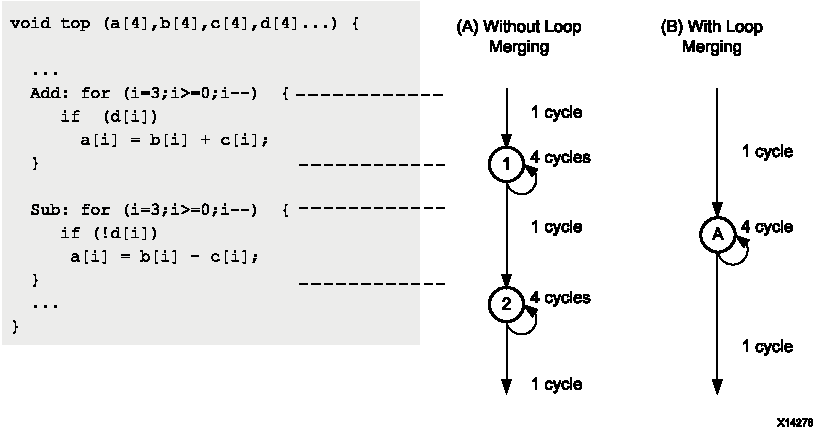
\includegraphics[scale=0.8]{./Figures/HLS17.pdf}
  \caption{Funcionamiento de la Directiva LOOP MERGE \citep{HLS2015}}
  \label{fig:HLS17}
\end{figure}

En este caso, sin la aplicación de la directiva, vemos que al sistema le toma 5 ciclos extra con respecto a aplicar la directiva al código fuente, pues se combinan ambos bucles en un solo estado de ejecución.

Es importante tener en cuenta que la directiva LOOP\_MERGE es únicamente aplicable si los bucles no cuentan con ningún tipo de dependencia entre sí.

La directiva PIPELINE provista por el software le da la posibilidad al diseñador de agregar etapas de pipeline a la ejecución de funciones y bucles dentro del código fuente del circuito a sintetizar; esta directiva se encarga de adicionar los estados de la unidad de control y el hardware necesario para el funcionamiento.

Como se describió anteriormente, la directiva PIPELINE puede ser aplicada tanto en funciones como en bucles. En la Figura \ref{fig:HLS18} se puede apreciar el comportamiento de la directiva aplicada a funciones en la parte izquierda y el comportamiento de la directiva aplicada a bucles en la parte derecha. En la parte inferior tenemos el comportamiento de las peticiones de lectura y escritura producido por ambas implementaciones. En el caso de aplicar la directiva a bucles, podemos notar que la unidad de control debe adicionar burbujas y liberar los registros cuando se requiere iniciar una nueva iteración del bucle. Esta, aunque es una operación necesaria, puede incrementar la latencia del circuito.

\begin{figure}[H]
  \centering
    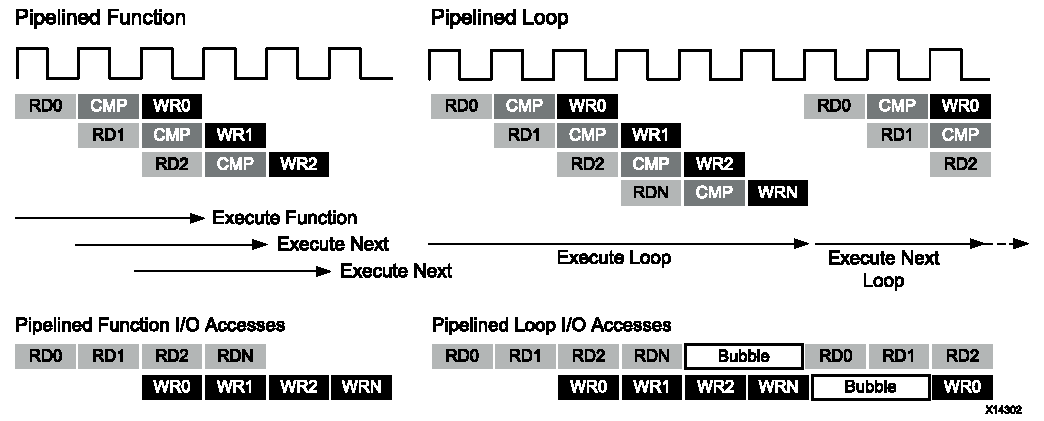
\includegraphics[scale=0.8]{./Figures/HLS18.pdf}
  \caption{Directiva PIPELINE aplicada a funciones y bucles \citep{HLS2015}}
  \label{fig:HLS18}
\end{figure}

La aplicación de la directiva PIPELINE provee al diseñador la capacidad de explotar en mayor medida el hardware que se está diseñando. Sin embargo, esta directiva trae consigo problemas como la adición de burbujas que claramente incrementan la latencia y el hecho de que el sistema deba desocupar el pipeline cuando los datos no estén disponibles para ser computados por el hardware; estos problemas pueden ser solucionados fácilmente con los modos PIPELINE\_REWIND y PIPELINE\_FLUSH respectivamente.

La Figura \ref{fig:HLS19} nos muestra el comportamiento de la directiva PIPELINE en su modo REWIND.

\begin{figure}[H]
  \centering
    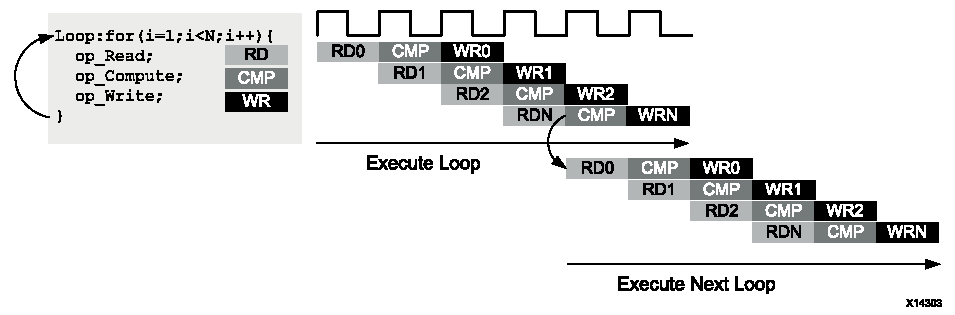
\includegraphics[scale=0.8]{./Figures/HLS19.pdf}
  \caption{Comportamiento del modo PIPELINE\_REWIND  \citep{HLS2015}}
  \label{fig:HLS19}
\end{figure}

Este modo permite reducir la latencia del circuito al ejecutar bucles, pues no requiere agregar burbujas ni evacuar las etapas del pipeline para continuar con la siguiente iteración. Este tipo de modos requiere una gran cantidad de hardware para su implementación y más aún cuando se realizan operaciones complicadas con bucles anidados. Es posible entonces que el sintetizador no pueda aplicar la directiva con este modo dada la complejidad y las dependencias de datos.

Otro de los problemas del pipeline es la dependencia de datos. La dependencia de datos cuando se corre un circuito con pipeline implica que este no puede continuar con las operaciones hasta que los datos se encuentren disponibles provocando que las etapas del pipe sean evacuadas. Esto trae consigo un incremento de la latencia, pues idealmente estas etapas deberían permanecer llenas. Con la aplicación del modo FLUSH de la directiva PIPELINE este tipo de eventos no provocará la evacuación de las etapas del pipeline, pues la unidad de control detecta el momento en que los recursos no se encuentran disponibles y congela la ejecución del hardware hasta que los datos se encuentran disponibles para ser computados nuevamente por el hardware; ver Figura \ref{fig:HLS3}.

\begin{figure}[H]
  \centering
    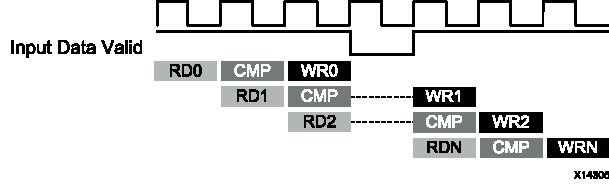
\includegraphics[scale=0.8]{./Figures/HLS3.pdf}
  \caption{Comportamiento del modo PIPELINE\_FLUSH \citep{HLS2015}}
  \label{fig:HLS3}
\end{figure}

Continuando con las directivas que favorecen la concurrencia encontramos la directiva UNROLL. Esta directiva permite dividir el hardware de un bucle especificando un factor de división. El factor de división de la directiva por omisión es un unroll de tamaño completo; ver Figura \ref{fig:HLS4}. Cada una de las divisiones que se realizan usando la directiva UNROLL crea instancias nuevas con los mismos recursos de hardware que el circuito original; la diferencia radica en la unidad de control y la forma en que se administra la ejecución del algoritmo usando las diferentes particiones; ver Figura \ref{fig:HLS4}.

\begin{figure}[H]
	\centering
		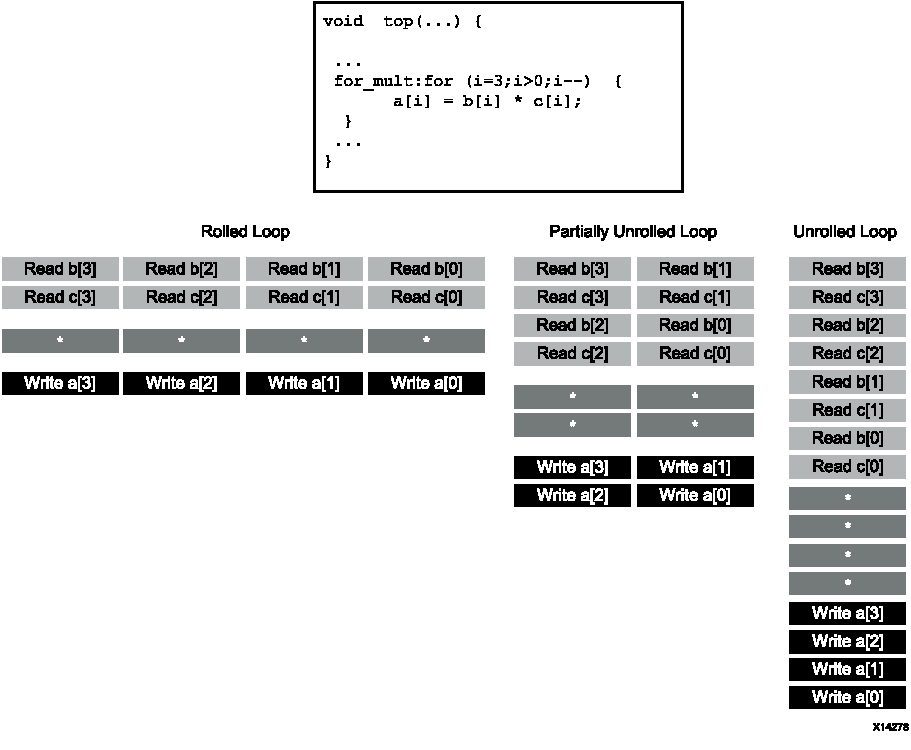
\includegraphics[scale=0.8]{./Figures/HLS4.pdf}
	\caption{Funcionamiento de la Directiva UNROLL \citep{HLS2015}}
	\label{fig:HLS4}
\end{figure}

Un bucle puede tener tres estados. El más común es el estado natural en el cual no se ha aplicado la directiva; este caso se conoce como un ROLLED LOOP. El segundo estado es aplicando la directiva con factor de dos o más; este estado se conoce como PARTIALLY UNROLLED LOOP. Finalmente el estado ideal, que implica consumir grandes cantidades de hardware es el FULLY UNROLLED LOOP; en este caso, cada una de las operaciones del circuito se realiza en un hardware dedicado.

La directiva UNROLL es capaz de reducir considerablemente la latencia del circuito tras su aplicación, pero su aplicación puede traer consecuencias como cuellos de botella si las memorias BRAM no han sido particionadas correctamente.

La directiva CLOCK es muy importante cuando se diseña usando HLS pues esta, permite al diseñador usar diferentes dominios de tiempo para cada uno de sus circuitos y funciones dentro del mismo módulo. Esto le da la libertad de validar el funcionamiento de su circuito con diferentes frecuencias de reloj, lo cual, si se aprovecha, puede incrementar el rendimiento general del circuito.

Finalmente, Vivado HLS cuenta con la directiva INLINE. Esta directiva le permite al programador expandir en línea funciones pequeñas dentro de aquellas que las llaman con mayor frecuencia, con lo cual, la aplicación de esta directiva elimina ciclos de establecimiento de señales entre funciones además de eliminar el hardware de control de las interfaces de las funciones.

La mayoría de herramientas de síntesis de alto nivel permite crear directivas múltiples por dominio, dando la posibilidad de aplicar una o más directivas a una porción de código específica. Por ejemplo, a un bucle podría aplicarse directivas de PIPELINE y UNROLL al mismo tiempo, lo cual incrementaría el performance de la aplicación. La única restricción de este tipo de modificaciones usando directivas son las dependencias de datos; este tipo de problemas podría evitar que la directiva sea aplicada correctamente por el sintetizador.

\section{Software de Síntesis de Hardware Vivado Design Suite}

Aplicaciones como Vivado HLS, además de la síntesis de alto nivel y simulación del hardware, no permiten una implementación final en la FPGA. Para este fin existen herramientas de síntesis de hardware como \href{http://www.xilinx.com/products/design-tools/vivado.html}{Vivado Design Suite} \citep{Vivad98}; este software transforma el código en VHDL arrojado por la síntesis de alto nivel en un bitstream, el cual contiene la configuración de la lógica de la FPGA. Vivado Design Suite es un software complejo que conoce la arquitectura de la FPGA y se encarga de los aspectos de la optimización final de tiempo, área y potencia de la implementación deseada.

En la Figura \ref{fig:HLS9} se puede ver un ejemplo claro de cómo el software interconecta los bloques IP Core. En hardware es común ver que un bloque IP tenga múltiples interfaces de entrada y salida. Por ejemplo, un módulo que desee interactuar con una memoria BRAM deberá contar con señales de control compatibles con dicha RAM; conectar individualmente estas señales implica tiempo y si se habla de interfaces más complejas como las interfaces AXI, que requieren de 45 señales en su formato FULL AXI4, la conexión requerirá aún más tiempo. Vivado Design Suite reconoce la interface de cada IP Core y las agrupa, permitiendo así realizar una sola conexión por interface.

\begin{figure}[H]
  \centering
    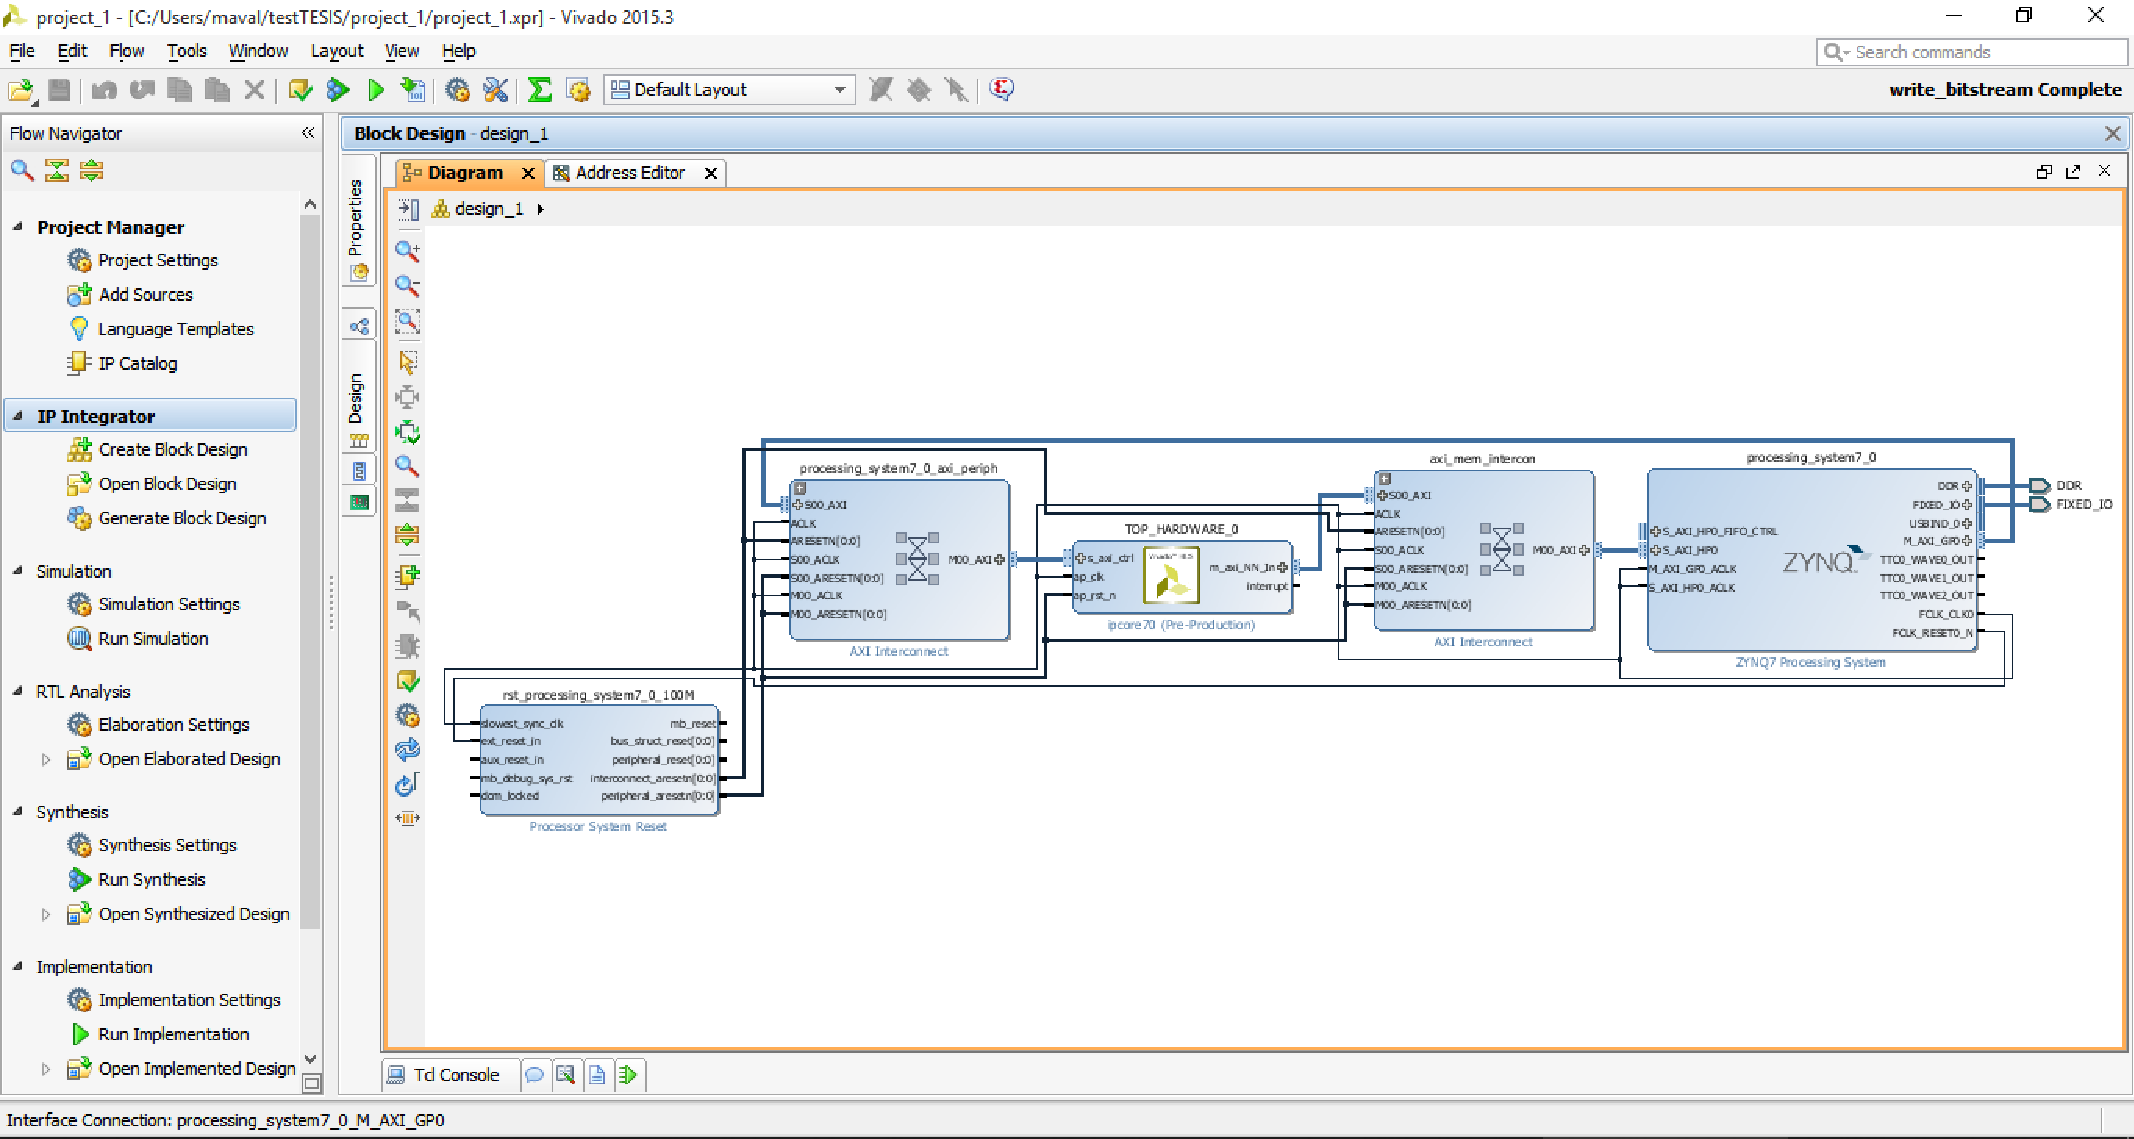
\includegraphics[scale=0.4]{./Figures/HLS9.pdf}
  \caption{Vivado Design Suite GUI}
  \label{fig:HLS9}
\end{figure}

En el caso de las interfaces mapeadas a memoria como las interfaces AXI, Vivado Design Suite se encarga de mostrarle al disenador el lugar de la memoria donde el sistema será mapeado; esto se hace según la Tabla \ref{tab:DIR}. Dependiendo del puerto al que se ha conectado el módulo al procesador ARM, quien es el que tiene el controlador de la memoria RAM DDR3, la herramienta entregará un rango de memoria disponible para el usuario.

% \begin{table}[H]
% \centering
% \begin{tabular}{|l|l|l|l|l|l|}
% \hline
% \textbf{Cell} & \textbf{Slave Interface} & \textbf{Base Name} & \textbf{Offset Address} & \textbf{Range} & \textbf{High Address} \\ \hline
% \multicolumn{6}{|l|}{processing\_system7\_0} \\ \hline
% \multicolumn{6}{|l|}{Data (32 address bits : 0x40000000 {[} 1G {]})} \\ \hline
% \multicolumn{6}{|l|}{M\_AXI\_GP0} \\ \hline
% TOPANN\_0 & s\_axi\_AXILiteS & Reg & 0x43C0\_0000 & 64K & 0x43C0\_FFFF \\ \hline
% \multicolumn{6}{|l|}{TOPANN\_0} \\ \hline
% \multicolumn{6}{|l|}{Data\_m\_axi\_INPUTS (32 address bits : 4G)} \\ \hline
% \multicolumn{6}{|l|}{m\_axi\_INPUTS} \\ \hline
% processing\_system7\_0 & S\_AXI\_HP0 & \begin{tabular}[c]{@{}l@{}}HP0\_DDR\_\\ LOWOCM\end{tabular} & 0x0000\_0000 & 512M & 0x1FFF\_FFFF \\ \hline
% \multicolumn{6}{|l|}{Data\_m\_axi\_OUTPUTS (32 address bits : 4G)} \\ \hline
% \multicolumn{6}{|l|}{m\_axi\_OUTPUTS} \\ \hline
% processing\_system7\_0 & S\_AXI\_HP0 & \begin{tabular}[c]{@{}l@{}}HP0\_DDR\_\\ LOWOCM\end{tabular} & 0x0000\_0000 & 512M & 0x1FFF\_FFFF \\ \hline
% \end{tabular}
% \caption{Mapeo de direcciones del Zynq 7000}
% \label{tab:DIR}
% \end{table}

\begin{table}[H]
\centering
\resizebox{\columnwidth}{!}{
\begin{tabular}{|l|c|c|c|l|}
\hline
\multicolumn{1}{|c|}{\textbf{Address Range}} & \textbf{CPUs y ACP} & \textbf{AXI\_HP} & \textbf{Others Bus Master} & \multicolumn{1}{c|}{\textbf{Notas}}                                                             \\ \hline
\multirow{4}{*}{0000\_0000 to 0003\_FFFF}   & OCM                 & OCM              & OCM                        & Address not filtered by SCU and OCM is mapped low                                               \\ \cline{2-5} 
                                            & DDR                 & OCM              & OCM                        & \begin{tabular}[c]{@{}l@{}}Address filtered by SCU and OCM is\\ mapped low\end{tabular}         \\ \cline{2-5} 
                                            & DDR                 &                  &                            & \begin{tabular}[c]{@{}l@{}}Address filtered by SCU and OCM is not\\ mapped low\end{tabular}     \\ \cline{2-5} 
                                            &                     &                  &                            & \begin{tabular}[c]{@{}l@{}}Address not filtered by SCU and OCM is\\ not mapped low\end{tabular} \\ \hline
\multirow{2}{*}{0004\_0000 to 0007\_FFFF}   & DDR                 &                  &                            & Address filtered by SCU                                                                         \\ \cline{2-5} 
                                            &                     &                  &                            & Address not filtered by SCU                                                                     \\ \hline
\multirow{2}{*}{0008\_0000 to 000F\_FFFF}   & DDR                 & DDR              & DDR                        & Address filtered by SCU                                                                         \\ \cline{2-5} 
                                            &                     & DDR              & DDR                        & Address not filtered by SCU                                                                     \\ \hline
0010\_0000 to 3FFF\_FFFF                    & DDR                 & DDR              & DDR                        & Accessible to all interconnect masters                                                          \\ \hline
4000\_0000 to 7FFF\_FFFF                    & PL                  &                  & PL                         & \begin{tabular}[c]{@{}l@{}}General Purpose Port \#0 to the PL,\\ M\_AXI\_GP0\end{tabular}       \\ \hline
8000\_0000 to BFFF\_FFFF                    & PL                  &                  & PL                         & \begin{tabular}[c]{@{}l@{}}General Purpose Port \#1 to the PL,\\ M\_AXI\_GP1\end{tabular}       \\ \hline
E000\_0000 to E02F\_FFFF                    & IOP                 &                  & IOP                        & I/O Peripheral registers                                                                        \\ \hline
E100\_0000 to E5FF\_FFFF                    & SMC                 &                  & SMC                        & SMC Memories                                                                                    \\ \hline
F800\_0000 to F800\_0BFF                    & SLCR                &                  & SLCR                       & SLCR registers                                                                                  \\ \hline
F800\_1000 to F880\_FFFF                    & PS                  &                  & PS                         & PS System registers                                                                             \\ \hline
F890\_0000 to F8F0\_2FFF                    & CPU                 &                  &                            & CPU Private registers                                                                           \\ \hline
FC00\_0000 to FDFF\_FFFF                    & Quad-SPI            &                  & Quad-SPI                   & Quad-SPI linear address for linear mode                                                         \\ \hline
\multirow{2}{*}{FFFC\_0000 to FFFF\_FFFF}   & OCM                 & OCM              & OCM                        & OCM is mapped high                                                                              \\ \cline{2-5} 
                                            &                     &                  &                            & OCM is not mapped high                                                                          \\ \hline
\end{tabular}
}
\caption{Mapa de Direcciones del Zynq 7000 Processing System \citep{TRM2017}}
\label{tab:DIR}
\end{table}

\section{Red Neuronal Artificial}

Las redes neuronales (\textit{ANN}, por las siglas en inglés de \textit{Artificial Neural Network}), han surgido como un mecanismo para solucionar problemas en diferentes ámbitos. Esto se debe a que estas tienen la capacidad de diagnosticar, detectar, predecir, monitorear, entre otras tareas \citep{amato2013artificial,singh2009artificial,sivapathasekaran2010artificial,kiani2010application}. La principal ventaja de estos sistemas es la facilidad que tienen para adaptarse a las necesidades de un problema. Solo se necesita un buen entrenamiento y una buena topología para que pueda cumplir con las exigencias del proyecto.

Para el desarrollo de ANN, existen dos técnicas muy conocidas, tanto para el entrenamiento como para la topología. La primera es \textit{BPA} \textit{(Back-Propagation Algorithm)}. Permite propagar el error de la salida por cada una de las capas de la red, de forma que el error de la salida se va reduciendo debido a la modificación de los pesos sinápticos. La segunda es \textit{MLP} \textit{(Multi-Layer Perceptron)}; esta es históricamente la más usada para el desarrollo de redes. Esto es debido a los buenos resultados que se han obtenido al implementarla \citep{wilamowski2009neural}.

\subsection{Neurona Básica}

Una neurona artificial o perceptrón es un modelo matemático basado en su contraparte biológica. Una neurona es una célula compuesta por una cantidad indefinida de conductos de entrada llamados dendritas y un conducto de salida llamado axón. Los conductos le permiten a la neurona comunicarse con otras neuronas, de forma que las señales de los sensores de entrada se van propagando a través de cada una. El perceptrón es la unidad de procesamiento básico de una ANN; está compuesto por cuatro partes esenciales: nodos de entrada, pesos sinápticos, función de propagación y función de salida, como se muestra en la Figura \ref{fig:neurona}.

\begin{figure}[H]
\centering
\begin{tikzpicture}[
cirt/.style={
  draw,
  circle,
  inner sep=2pt,
  font=\normalsize,
  join = by -latex
},
init/.style={
  draw,
  circle,
  inner sep=2pt,
  font=\Huge,
  join = by -latex
},
squa/.style={
  draw,
  inner sep=5pt,
  font=\Large,
  join = by -latex
}
]
\begin{scope}[start chain=1,node distance=13mm]
\node[on chain=1] at (0,1.5cm) 
  (x1) {$x_1$};
\node[on chain=1,cirt] 
  (w1) {$w_1$};
\end{scope}

\begin{scope}[start chain=2,node distance=13mm]
\node[on chain=2] at (0,0.5cm) 
  (x2) {$x_2$};
\node[on chain=2,cirt] 
  (w2) {$w_2$};
\end{scope}

\begin{scope}[start chain=3,node distance=13mm]
\node[on chain=3] at (0,-0.5cm) 
  (xp) {$\vdots$};
\node[on chain=3] 
  (wp) {$\vdots$};
\end{scope}

\begin{scope}[start chain=4,node distance=13mm]
\node[on chain=4] at (0,-1.5cm) 
  (xn) {$x_n$};
\node[on chain=4,cirt,label=below:{\parbox{2cm}{\centering Pesos \\ sinápticos}}] 
  (wn) {$w_n$};
\end{scope}

\begin{scope}[start chain=5,node distance=13mm]
\node[on chain=5,init] at (4cm,0) (sigma) 
  {$\displaystyle\Sigma$};
\node[on chain=5,squa,label=above:{\parbox{2cm}{\centering Función de \\ activación}}](f){$\varphi(u)$};
\node[on chain=5,label=above:Salida,join=by -latex] (y)
  {$y$};
\end{scope}

\node[label=above:\parbox{2cm}{\centering Bias}] at (sigma|-w1) (b) {$\theta$};

\draw[-latex] (w1) -- (sigma);
\draw[-latex] (w2) -- (sigma);
\draw[-latex] (wn) -- (sigma);
\draw[-latex] (b) -- (sigma);
\draw[-latex] (sigma) to [edge node={node [sloped,above] {$u$}}] (f);
\draw[decorate,decoration={brace,mirror,amplitude=10pt}] (x1.north west) -- node[left=10pt] {Entradas} (xn.south west);
\end{tikzpicture}
\caption{Neurona básica}
\label{fig:neurona}
\end{figure}

\subsubsection{Función de Propagación}

Para el modelo matemático, las señales de entrada son expresadas por el conjunto $X=(x_1, x_2, x_3, \ldots, x_n)^T$. Para simular el proceso de reorganización de las conexiones sinápticas de las neuronas biológicas, se asocia a cada elemento del conjunto de entrada un peso sináptico que le permite darle a la conexión un valor de excitación o de inhibición dependiendo del signo. Los pesos sinápticos se expresan por el conjunto $W=(w_1, w_2, w_3, \ldots, w_n)^T$.

La función de propagación se encarga de multiplicar el conjunto de entrada y el conjunto de pesos sinápticos, término a término, para luego hacer la sumatoria de los elementos del vector resultante y así generar un valor de salida, $u$. La expresión completa para la función de propagación está dada por la Ecuación \ref{eq:funpro}

\begin{equation}\label{eq:funpro}
  u=\sum_{i=1}^{n} w_ix_i + \theta
\end{equation}

donde $x_i \in X$, $w_i \in W$ y $\theta$ es el umbral de inhibición o excitación de la neurona.

\subsubsection{Función de  Activación}

La función de activación surge como una necesidad de tener una salida de la neurona acotada a un rango determinado; esto se debe a que la salida en la neurona biológica se encuentra acotada en amplitud. En la Ecuación \ref{eq:func} se muestra la expresión matemática respecto a $u$.

\begin{equation}\label{eq:func}
  y=\varphi(u)
\end{equation}

Existen diferentes tipos de funciones de activación. La elección de estas depende del objetivo del diseño:

\begin{table}[H]
\centering 
\renewcommand{\arraystretch}{1.8}
\begin{tabular}{| >{\centering\arraybackslash}m{2.4cm} | >{\arraybackslash}m{6cm}|}
\hline %inserts horizontal line
\textbf{Función de Activación} & \textbf{Expresión Matemática}\\ 
\hline 
Paso Unitario & $\varphi(u) = \begin{cases} 1.0 &\mbox{si } u > 0 \\ 
0.0 & \mbox{en otros casos}. \end{cases}$\\  \hline 
Rampa & $\varphi(u) = max \lbrace 0.0, min \lbrace 1.0, u+0.5 \rbrace \rbrace$\\ \hline 
Sigmoidal & $\varphi(u) = \dfrac{1}{1+e^{-u}}$\\ \hline 
Bipolar Sigmoid & $\varphi(u) = \dfrac{1-e^{-u}}{1+e^{-u}}$\\ \hline 
Tangente Sigmoidal & $\varphi(u) = \dfrac{2}{1+e^{-2u}}-1$\\ \hline 
\end{tabular}
\caption{Funciones de Activación}
\label{tab:funactivacion}
\end{table}

\subsection{Perceptrón Multi-Capa}

Un MLP \textit{Multilayer Perceptron} es una red de neuronas que está compuesta por una capa de nodos de entrada, una o dos capas ocultas y una capa de salida. Todas las capas están compuestas por neuronas artificiales a excepción de la capa de entrada donde los nodos son las señales de ingreso a la red. Las conexiones entre capas dependen de la configuración de la red; puede ser completamente conectada si cada uno de los nodos de una capa se conecta con todos los nodos de la siguiente, véase Figura \ref{fig:MLP}. Por otro lado, puede tener una conexión personalizada y no estar completamente conectada.

\begin{figure}[H]
\centering
\begin{tikzpicture}[x=1.5cm, y=1.5cm,
every neuron/.style={
    circle,
    draw,
    minimum size=0.7cm
  },
every input/.style={
    draw,
  },
every layer/.style={
    draw=none, 
    scale=2,
    execute at begin node=\color{black}$\ldots$
  },
neuron missing/.style={
    draw=none, 
    scale=2,
    text height=0.25cm,
    execute at begin node=\color{black}$\vdots$
  }
]
\foreach \m/\l [count=\y] in {1,2,missing,3}
  \node [every input/.try, neuron \m/.try] (input-\m) at (0,2.5-\y*0.85) {};

\foreach \m [count=\y] in {1,2,missing,3}
  \node [every neuron/.try, neuron \m/.try ] (hidden1-\m) at (1.5,2.5-\y*0.85) {};

\foreach \m [count=\y] in {1,2,3,4}
  \node [every layer/.try] (empty-\m) at (2.5,2.5-\y*0.8) {};
  
  \foreach \m [count=\y] in {1,2,missing,3}
  \node [every neuron/.try, neuron \m/.try ] (hidden2-\m) at (3.5,2.5-\y*0.85) {};

\foreach \m [count=\y] in {1,2,missing,3}
  \node [every neuron/.try, neuron \m/.try ] (output-\m) at (5,2.5-\y*0.85) {};

\foreach \l [count=\i] in {1,2,n}
  \draw [latex-] (input-\i) -- ++(-1,0)
    node [above, midway] {$x_\l$};

\foreach \l [count=\i] in {1,2,n}
  \node [above] at (hidden1-\i.south) {$n_\l$};

\foreach \l [count=\i] in {1,2,n}
  \draw [-latex] (output-\i) -- ++(1,0)
    node [above, midway] {$s_\l$};

\foreach \i in {1,...,3}
  \foreach \j in {1,...,3}
    \draw [-latex] (input-\i) -- (hidden1-\j);

\foreach \i in {1,...,3}
  \foreach \j in {1,...,3}
    \draw [-latex] (hidden2-\i) -- (output-\j);

\node [align=center, above] at (0,2.25) {Capa de \\ entrada};
\node [align=center, above] at (2.5,2.25) {Capas \\ ocultas};
\node [align=center, above] at (5,2.25) {Capa de \\ salida};
\draw [decorate,decoration={brace,amplitude=10pt}] (1.2,2) -- (3.8,2);
\end{tikzpicture}
\caption{MLP completamente conectada}
\label{fig:MLP}
\end{figure} % Marco Téorico 

\chapter{Recursos} % Write in your own chapter title
\label{Chapter7}
\lhead{Capítulo 7. \emph{Recursos}} % Write in your own chapter title to set the page header

\section{Hardware}

\begin{itemize}
\item \href{https://store.digilentinc.com/zybo-zynq-7000-arm-fpga-soc-trainer-board/}{Tarjeta de Desarrollo ZYBO Zynq-7000 ARM/FPGA SoC}:
  \begin{itemize}
  \item Xilinx Zynq-7000 AP SoC XC7Z010-1CLG400C
    \begin{itemize}
    \item BRAM 18K: 120 Unidades.
    \item DSP48E: 80 Unidades.
    \item FF: 35200 Unidades.
    \item LUT: 17600 Unidades.
    \end{itemize}
  \item Dual-core ARM Cortex™-A9 
  \item 512 MB DDR3 
  \item 128 MB Quad-SPI Flash 
  \item 4 GB SD card 
  \item Onboard USB-JTAG Programming
  \item 10/100/1000 Ethernet 
  \item USB OTG 2.0 and USB-UART 
  \item Analog Devices ADAU1761 SigmaDSP® Stereo, Low Power, 96 kHz, 24-Bit Audio Codec
  \item Analog Devices ADV7511 High Performance 225 MHz HDMI Transmitter (1080p HDMI, 8-bit VGA, 128x32 OLED)
  \item PS \& PL I/O expansion (FMC, Pmod, XADC) 
  \end{itemize}
\end{itemize}

\section{Software}

\begin{itemize}
\item \href{http://www.xilinx.com/products/design-tools/vivado.html}{Vivado Design Suite 2017.4} \citep{Vivad98}: Programa para síntesis e implementación de hardware a partir de una descripción usando VHDL o Verilog.
\item \href{http://www.xilinx.com/products/design-tools/vivado/integration/esl-design.html}{Vivado HLS 2017.4} \citep{Vivad77}: Programa para síntesis de alto nivel a un lenguaje de descripción de hardware (VHDL o Verilog).
\item \href{http://www.xilinx.com/products/design-tools/embedded-software/petalinux-sdk.html}{Petalinux SDK 17.4} \citep{PetaL29}.
\item \href{http://www.putty.org}{PuTTY} \citep{Put}.
\end{itemize}

 % Metodología 

% Chapter 8

\chapter{Metodología} % Write in your own chapter title
\label{Chapter8}
\lhead{Capítulo 8. \emph{Metodología}} % Write in your own chapter title to set the page header

Para el desarrollo de  los objetivos se seguirán los siguientes lineamientos.
\begin{enumerate}
\item \textbf{Aplicación de la computación consciente del contexto}
\begin{itemize}
\item \textit{Aplicación de algoritmo de procesamiento de datos y escalamiento de hardware}: Una vez definidos los algoritmos a usar, se desarrollarán inicialmente en un lenguaje de programación como C/C++, los cuales servirán como insumo para el producto final usando HLS.
\item \textit{Comparación de algoritmos}: Se realizará una comparación de los algoritmos según la cantidad de sensores a fusionar.
\item \textit{Escritura}: Documentar los hallazgos encontrados.
\end{itemize}

\item \textbf{Elección de la plataforma de computación para IoT que permita reconfiguración parcial dinámica}
\begin{itemize}
\item \textit{Búsqueda tarjeta de desarrollo}: Se consultan las diferentes tarjetas de desarrollo hardware disponibles con programación en alto nivel.

\item \textit{Verificación}: Se realiza un análisis de compatibilidad entre lenguajes de programación y herramientas disponibles.
\item \textit{Escritura}: Se especifica la arquitectura y herramientas a usar.
\end{itemize}
\item \textbf{Integración de los diferentes módulos dentro de la plataforma de procesamiento usando síntesis de alto nivel}
\begin{itemize}
\item \textit{Programación HLS}: Se programan los algoritmos de fusión usando síntesis de alto nivel HLS.
\item \textit{Programación RP}: Se realiza la configuración de los módulos que harán uso de la reconfiguración parcial.
\item \textit{Escritura}: Se reportan los recursos y métodos de hardware usados para la implementación.
\end{itemize}
\item \textbf{Comparar el rendimiento de la plataforma desarrollada con una implementación diseñada completamente en software}
\begin{itemize}
\item \textit{Pruebas iniciales}: Se realiza la verificación de funcionamiento del sistema completo.
\item \textit{Correcciones}: Se corrigen posibles errores de implementación y diseño.
\item \textit{Pruebas finales}: Se realizan pruebas de rendimiento y funcionalidad del sistema en su última etapa.
\item \textit{Evaluación final}: Se evalúa el desempeño del sistema en su totalidad, con lo cual se obtienen los resultados a reportar en el documento.
\item \textit{Escritura}: Se reportan los resultados obtenidos.
\end{itemize}
\end{enumerate}

   % Recursos 

\chapter{Elección de la Plataforma de Desarrollo} % Write in your own chapter title
\label{Chapter9}
\lhead{Capítulo 9. \emph{Plataforma}} % Write in your own chapter title to set the page header

\section{Elección de la plataforma}

Se realiza un análisis primario con las familias de FPGA disponibles comercialmente por Xilinx que permiten reconfiguración dinámica y la instrumentación necesaria para servir como Gateway de IoT como la posibilidad de correr un SO y conexión a red.

La Tabla \ref{fpgaFamilies} muestra las familias de SoC dentro de la categoría de precio reducido y rendimiento medio. Se nota que por cantidad de recursos la opción mas viable es la familia ZYNQ 7000, ofreciendo hasta el doble de celdas lógicas y casi tres veces la cantidad de DSPs que otras plataformas dentro de su categoría, volviéndola rápidamente la familia a examinar.

\begin{table}[!ht]
\centering
\resizebox{\textwidth}{!}{%
\begin{tabular}{|l|c|c|c|}
\hline
\multicolumn{1}{|c|}{\textbf{SoC}} & \textbf{ZYNQ 7K} & \textbf{ARTIX 7} & \textbf{SPARTAN 7} \\ \hline
MAX LOGIC CELLS [k] & 444 & 215 & 102 \\ \hline
MAX MEM [Mb] & 26.5 & 13 & 4.2 \\ \hline
DSPs & 2020 & 740 & 160 \\ \hline
TRANSCEIVER SPEEDS [Gb/s] & 12.5 & 6.6 & NA \\ \hline
MAX I/O PINS & 250 & 500 & 400 \\ \hline
\end{tabular}%
}
\caption{Familias de FPGA}
\label{fpgaFamilies}
\end{table}

La Tabla \ref{fpgaComparison} muestra las diferentes plataformas de desarrollo  disponibles y de fabricantes como AVNET y DIGILENT. En ella vemos que los diferentes SoC de cada una de las plataformas cuentan con diferentes recursos de hardware y características extra adicionadas por el fabricante.

\begin{table}[!ht]
\small
\centering
\begin{adjustbox}{width=1.1\textwidth}
\small
\begin{tabular}{|l|c|c|c|c|c|c|c|c|c|c|}
\hline
\multicolumn{1}{|c|}{\textbf{Nombre}} & \textbf{X Z7K EKIT} & \textbf{MICROZED} & \textbf{PICOZED} & \textbf{ZEDBOARD} & \textbf{MINIZED} & \textbf{PYNQ-Z1} & \textbf{ZYBO N} & \textbf{ZYBO O} \\ \hline
\textbf{SoC} & ZC702 & ZC7010 & ZCZ010 & XC7Z020 & XC7Z007S & XC7Z020 & XC7Z020 & XC7Z010 \\ \hline
\textbf{Price} & 895 & 266 & 178 & 475 & 89 & 199 & 299 & 199 \\ \hline
\textbf{Max LogicCells} & 85000 & 28000 & 28000 & 85000 & 23000 & 53200 & 53200 & 28000 \\ \hline
\textbf{Max BRAM Mb} & 4.9 & 1.92 & 1.92 & 4.9 & 1.8 & 4.9 & 4.9 & 1.92 \\ \hline
\textbf{DSPs} & 220 & 80 & 80 & 220 & 66 & 220 & 220 & 80 \\ \hline
\textbf{DDR RAM MB} & 1024 & 1024 & 1024 & 512 & 512 & 512 & 1024 & 512 \\ \hline
\textbf{Notas} &  &  & No headers &  & No headers &  &  &  \\ \hline
\end{tabular}%
\end{adjustbox}
\caption{Comparación tarjetas de desarrollo}
\label{fpgaComparison}
\end{table}

Para elegir la plataforma de desarrollo ideal se debe tener en cuenta el objetivo de lo que se está desarrollando y más importante aún, el para qué se está desarrollando. En este caso, se desea implementar un algoritmo altamente concurrente con el objetivo de operar bajo un esquema de IoT. Por lo tanto, es importante tener en cuenta que se requiere que los recursos de hardware sean altos, que tenga un stack de red y los jacks de conexión, todo esto bajo un kernel de Linux que permita administración remota usando SSH. Desde esta óptica, la mayoría de tarjetas cumplen con los requisitos. Algunas, como las Picozed y Minized, del fabricante AVNet no cuentan con el jack RJ45 de red, entre otros headers; para estas tarjetas, es necesario adicionar accesorios que incrementarían el precio base. Finalmente, se debe tener en cuenta el precio y el soporte del fabricante. En este caso, basado en la cantidad de recursos y el precio, la mejor plataforma sería la \textbf{PYNQ-Z1}. Aunque cuenta con 512MB de RAM DDR3, por su precio es imbatible frente a las otras plataformas; de requerirse más memoria RAM, la mejor opción sería la versión nueva de ZYBO, ambas del fabricante DIGILENT.

Dentro de este esquema de desarrollo es necesario aclarar que independientemente de la plataforma de desarrollo elegida, la implementación debería ser transversal a todas las familias de Xilinx que usen VIVADO como sintetizador de hardware, siendo las diferencias entre los SoC la velocidad de transferencia y eficiencia de la FPGA en el diseño de sus bloques lógicos, pudiendo obtener latencias más bajas en FPGAs más costosas.
 % Cronograma 

% Chapter 10

\chapter{Diseño de Software y Hardware} % Write in your own chapter title
\label{Chapter10}
\lhead{Capítulo 10. \emph{Diseño}} % Write in your own chapter title to set the page header

La investigación basada en el estado del arte Capítulo \ref{Chapter6}, determinó que la estructura que mejor se acopla al tipo de problema es una ANN de tres capas, tres neuronas en la capa de entrada para analizar las variables de Flujo, Precipitación y Humedad Relativa, una capa oculta con mínimo tres neuronas y finalmente una neurona en la capa de salida. Por otra parte, también determinó que es necesario escalar el sistema de detección proporcionalmente según la necesidad de resolución en la medición, esto es necesario cuando se desea determinar con mayor precisión el riesgo de inundación del área examinada.

%Dado el problema, según el estado del arte, la mejor estructura de análisis es una Red Neuronal Artificial que pueda recibir al menos 3 datos (Flujo, Precipitación y Humedad Relativa) por nodo de medición. Esta medición debe ser instantánea y dependiendo de las condiciones meteorológicas; es decir, si la probabilidad de una inundación incrementa analizar los datos de los múltiples nodos que componen el ecosistema de monitoreo del río a una frecuencia mas alta, de forma concurrente y poder responder a tiempo ante una emergencia alertando al centro de control local. 

%tek Revisar redacción...

\section{Diseño de Hardware}

Diseñar el hardware implica tener en cuenta las diferentes etapas del desarrollo del mismo; en este caso, es necesario conocer cómo funcionan el sintetizador de alto nivel Vivado HLS y el sintetizador de hardware Vivado Design Suite. Se estableció una metodología que permite establecer el mejor diseño de hardware: en primera instancia se debe realizar un análisis de cuáles son las posibles optimizaciones que puedan reducir la latencia total del circuito una vez sintetizado y cuáles podrían incrementarla.

\begin{enumerate}
\item Desarrollar la ANN usando lenguage C++.
\item Sintetizar el hardware usando Vivado HLS.
\item Analizar latencia y uso de recursos obtenidos en el reporte.
\item Aplicar optimizaciones de hardware.
\item Repetir desde 2 hasta obtener el mínimo entre latencia y uso de recursos.
\end{enumerate}

Para este circuito se determinó que la latencia mínima se podría obtener usando las siguientes optmizaciones luego de analizar el código de la ANN, los bloques de memoria requeridos para realizar los bursts de memoria que provee la interfaz AXI, la cantidad de bucles y la cantidad de tareas que se realizan al interior del hardware.

\begin{enumerate}
\item Dataflow: Aplicable a tareas
\item Pipeline: Aplicable a bucles
\item Unroll: Aplicable a bucles
\end{enumerate}

\subsection{Diseño de la Red Neuronal Artificial}

Como se mencionó en el Capítulo \ref{Chapter7}, las redes neuronales son sistemas concurrentes capaces de aprender y realizar tareas para las que han sido entrenadas; por ejemplo, detección de patrones, clasificación, implementación de modelos matemáticos y fusión de datos. Por esta razón, es que se decide aplicarla a este problema, pues se desconoce la interacción entre las variables meteorológicas y físicas que afectan el nivel de los ríos provocando una inundación.

La Red Neuronal Artificial a implementar debe componerse de una capa de entrada con tres neuronas, un mínimo de tres neuronas en la capa oculta de la red y finalmente una neurona de salida, todo esto por nodo de medición en campo. Así pues, si se requieren analizar los datos provenientes de múltiples fuentes, se deberán instanciar tantas Redes Neuronales como nodos disponibles se tengan. La figura \ref{fig:networkDesign} muestra el diseño de la red implementada, en ella se puede observar el diseño básico, cada nodo de sensores se compone de una tripleta de neuronas a la entrada y en la capa oculta para ser por una neurona en la capa de salida la cual es la encargada de entregar el resultado de la estimación.

%La implementación de la red neuronal se compone de múltiples entradas totalmente conectadas entre sí; para el caso básico de muestreo se requieren como mínimo tres entradas y tres neuronas en la capa oculta. Para el caso en que se requieran analizar múltiples sensores, se deberían adicionar entradas tantos sensores se tengan disponibles y una capa oculta con igual número de neuronas como nodos de entrada a la red, véase la Figura \ref{fig:networkDesign}.

%tek Revisar redacción

\begin{figure}[H]
\centering
\begin{tikzpicture}[x=1.5cm, y=1.5cm,
every neuron/.style={ 
    circle,
    draw,
    minimum size=0.7cm
  },
every input/.style={
    draw,
  },
every layer/.style={
    draw=none, 
    scale=2,
    execute at begin node=\color{black}$\ldots$
  },
neuron missing/.style={
    draw=none, 
    scale=2,
    text height=0.25cm,
    execute at begin node=\color{black}$\vdots$
  }
]
\foreach \m/\l [count=\y] in {1,2,3,missing,4,5,6}
  \node [every input/.try, neuron \m/.try] (input-\m) at (-0.7,2.5-\y*0.85) {};

\foreach \m [count=\y] in {1,2,3,missing,4,5,6}
  \node [every neuron/.try, neuron \m/.try ] (hidden1-\m) at (1.5,2.5-\y*0.85) {};

% \foreach \m [count=\y] in {1,2,3,4}
%   \node [every layer/.try] (empty-\m) at (2.5,2.5-\y*0.8) {};
  
%   \foreach \m [count=\y] in {1,2,missing,3}
%   \node [every neuron/.try, neuron \m/.try ] (hidden2-\m) at (3.5,2.5-\y*0.85) {};
 
\foreach \m [count=\y] in {1}%,2,missing,3}
  \node [every neuron/.try, neuron \m/.try ] (output-\m) at (3.5,2.5-\y*1.7) {};

\foreach \l [count=\i] in {1,2,3,n1,n2,n3}
  \draw [latex-] (input-\i) -- ++(-1,0)
    node [above, midway] {$x_\l$};

\foreach \l [count=\i] in {1,2,3,n1,n2,n3}
  \node [above] at (hidden1-\i.south) {$h_\l$}; 

\foreach \l [count=\i] in {1}%,2,n}
  \draw [-latex] (output-\i) -- ++(1,0)
    node [above, midway] {$s_\l$};
  
\foreach \i in {1,...,6}
  \foreach \j in {1,...,6}
    \draw [-latex] (input-\i) -- (hidden1-\j);

\foreach \i in {1,...,6}
  \foreach \j in {1,...,1}
    \draw [-latex] (hidden1-\i) -- (output-\j);

\node [align=center, above] at (-0.7,2.25) {Capa de \\ entrada};
\node [align=center, above] at (1.5,2.25) {Capa \\ oculta};
\node [align=center, above] at (3.5,2.25) {Capa de \\ salida};
%\draw [decorate,decoration={brace,amplitude=10pt}] (1.2,2) -- (3.8,2);
\end{tikzpicture}
\caption{Diseño de la red neuronal}
\label{fig:networkDesign}
\end{figure}
 
\subsection{Función de salida de la red neuronal}

Uno de los parámetros que más influye en la veracidad de la estimación de una red neuronal es la función de activación de las neuronas, ver Tabla \ref{tab:funactivacion}. Según el estado del arte, la función de activación más común para este tipo de problemas es la función tangente sigmoidal \citep{floodfc1}, representada en la Ecuación \ref{eq:tansig} y la Figura \ref{fig:tansig}.

\begin{equation}\label{eq:tansig}
\varphi(u) = \dfrac{2}{1+e^{-2u}}-1
\end{equation}

\begin{figure}[H]
\centering
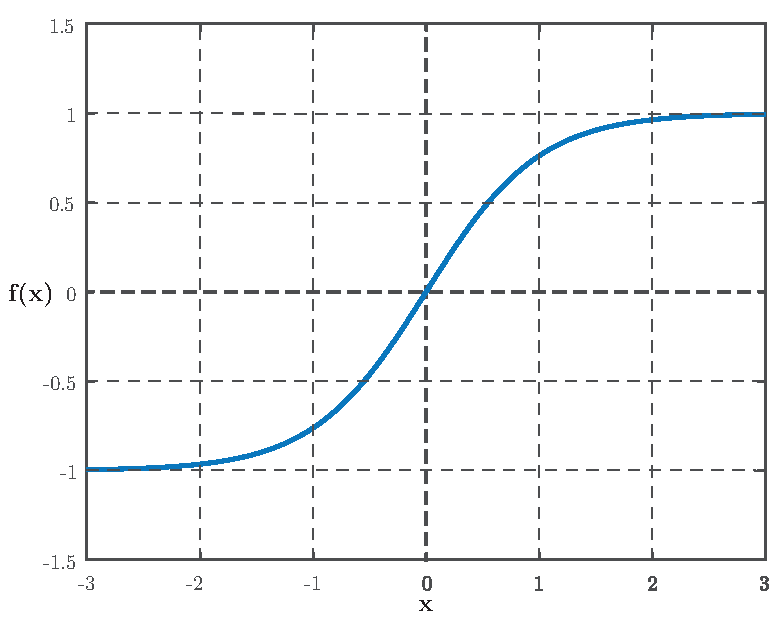
\includegraphics[scale=0.8]{./Figures/TANSIG.pdf}
\caption[Red neuronal en árbol]{Tangente sigmoidal}
\label{fig:tansig}
\end{figure}

La Ecuación \ref{eq:tansig} muestra que, para calcular la función tangente sigmoidal, es necesario realizar cómputos de complejos como los exponenciales que se pueden ver altamente afectados por el error que pueda introducir la unidad que los pueda calcular. Por otra parte, implementar este tipo de cálculos directamente sobre el hardware de la FPGA sería altamente costoso en términos de recursos y latencia por el simple hecho de utilizar punto flotante. Para resolver el problema se optó por realizar una implementación donde se discretiza la función continua, de tal forma que el bus de direcciones alcance máximo 12bits, es decir 4096 posiciones de memoria (se eligen 12b debido a que el sintetizador presenta problemas si se elige un bus de direcciones más grande al mapear una memoria ROM).

\subsection{Código fuente Red Neuronal Artificial}

A continuación se muestra de forma simplificada el diseño de la ANN en código fuente usando el lenguaje de programación C++

\begin{verbatim}
TOPANN ( fix *Inputs, fix *Outputs, fix *layerWeight, fix *layerBias,
  fix *outputLayerWeight, fix *outputLayerBias )
{  
  // Creación de buffers de memoria
  fix BurstInputs[DATASET_INPUTS];// Buffer local que garantiza el Burst
  fix layerResult[NEURONS];       // Permite reciclar el HW de las capas

  memcpy ( BurstInputs, (const fix *) Inputs,
    DATASET_INPUTS * sizeof(fix) );  // Mecanismo que activa el Burst
  
  // Ejecución del algoritmo de la ANN
  ANN ( BurstInputs, BurstOutputs, layerResult, Weights, ... )
  
  // Burst de salida
  memcpy ( (fix *) Outputs, layerResult, sizeof (fix) * OUTPUTS );
}
\end{verbatim}

Como se observa en el código anterior, la única diferencia entre una red de $3$ entradas y una de $N$ entradas son las definiciones de \texttt{DATASET\_INPUTS} y \texttt{NEURONS}, que definen respectivamente, cuántas entradas va a tener la red y la cantidad de neuronas en la capa oculta. Es por esto que se hace necesario sintetizar la cantidad de circuitos como variaciones de estas configuraciones.

\subsection{Puertos de entrada y salida AXI}

Dado que se requieren manipular grandes cantidades de datos provenientes de la red de sensores, se hace necesario que la ANN cuente con la instrumentación necesaria. En este caso, se optó por usar el máximo ancho de banda posible disponible en la arquitectura ZYNQ 7000; este es otorgado por el bus AMBA. Para lograr el máximo ancho de banda se requiere que el hardware realice un llamado en bloque a la memoria partiendo de una dirección base otorgada como dependencia en la entidad más alta como un apuntador (\texttt{* Inputs} y \texttt{* Outputs}) y realizar un llamado a la función \texttt{memcpy}, la cual activa el pipelining y las optimizaciones del bus en tiempo de síntesis; este proceso se conoce como MEMORY BURST TRANSACTION, véase la Figura \ref{fig:memBurst}.

\begin{figure}[H]
	\centering
		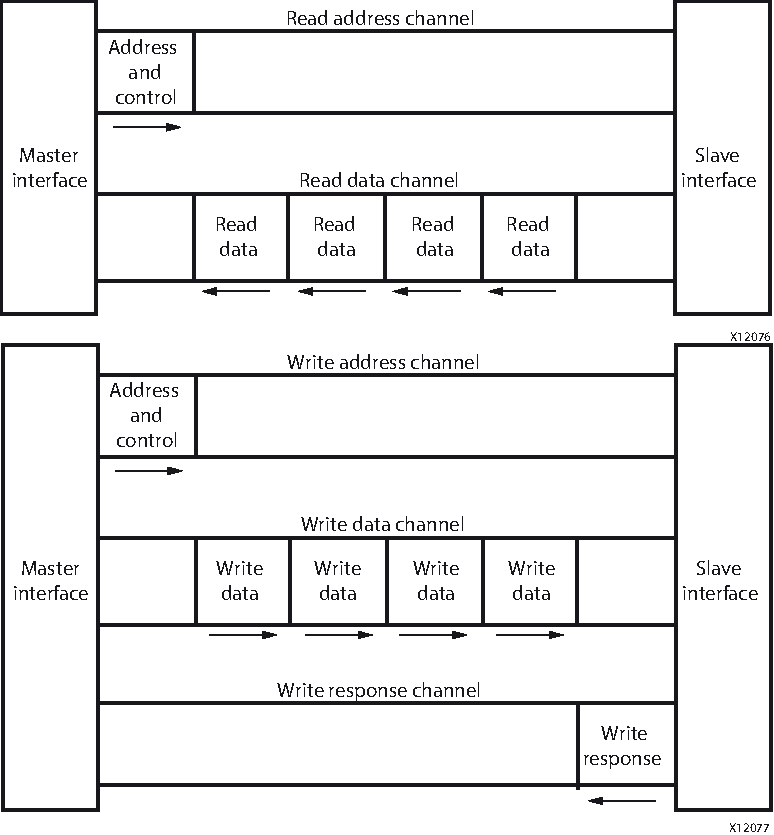
\includegraphics[scale=0.8]{./Figures/I2.pdf}
	\caption{Memory burst transaction \citep{AXI2017}}
	\label{fig:memBurst}
\end{figure}

Finalmente, es necesario determinar qué tipo de datos se usarán para realizar las operaciones a nivel de los datos. En este caso, para garantizar una baja latencia y un bajo uso de recursos, se optó por un ancho del bus de 32b definido en código como \texttt{fix}, el cual es una definición de 32b con 8b para la parte entera y 24b para la parte decimal, la cual puede ser ajustada de acuerdo a la necesidad.

\subsection{Optimizaciones de Hardware}

En la sub sección anterior se definió el diseño general de la ANN sin optimizaciones de hardware más allá de las dadas por la interfaz AXI. En esta sub sección se adicionarán las optmizaciones y los criterios de diseño para dejar una u otra optimización.

Previo a la síntesis, es necesario determinar cuáles son las optimizaciones adecuadas para el tipo de problema: del espectro de opciones, es necesario conocer bien el manual del Vivado HLS y las condiciones que deben cumplirse para aplicar las directivas, pues su disposición puede ser tanto positiva como negativa dependiendo de cómo se implementen. Tras analizar el código fuente, se estableció que, debido a la dependencia de los datos entre capas, el circuito se ve altamente beneficiado por mecanismos como el pipeline y el paralelismo de las diferentes tareas que se realizan. Una vez aplicadas las optimizaciones, es necesario analizar el reporte de síntesis y establecer si existen problemas con el ancho de banda de la memoria, el cual es un problema típico de este tipo de circuitos, en los que, debido a la alta concurrencia, el acceso a la RAM se ve afectado, teniendo que arbitrarse el acceso, aumentando en consecuencia de manera drástica la latencia total del circuito.

La Figura \ref{fig:latIntFloat} muestra la latencia e intervalo de datos para las diferentes optimizaciones. Estas están definidas en clocks y cada una brinda información importante para la implementación final; el intervalo indica cada cuántos clocks es posible introducir un nuevo dato al circuito para que pueda ser procesado y la latencia indica cuánto tarda un dato para ser procesado. En este caso, la combinación de las directivas DATAFLOW y PIPELINE permite obtener el menor intervalo en punto flotante, pero se ve superado por PIPELINE puro en cuanto a reducción de la latencia.

\begin{figure}[!ht]
	\centering
		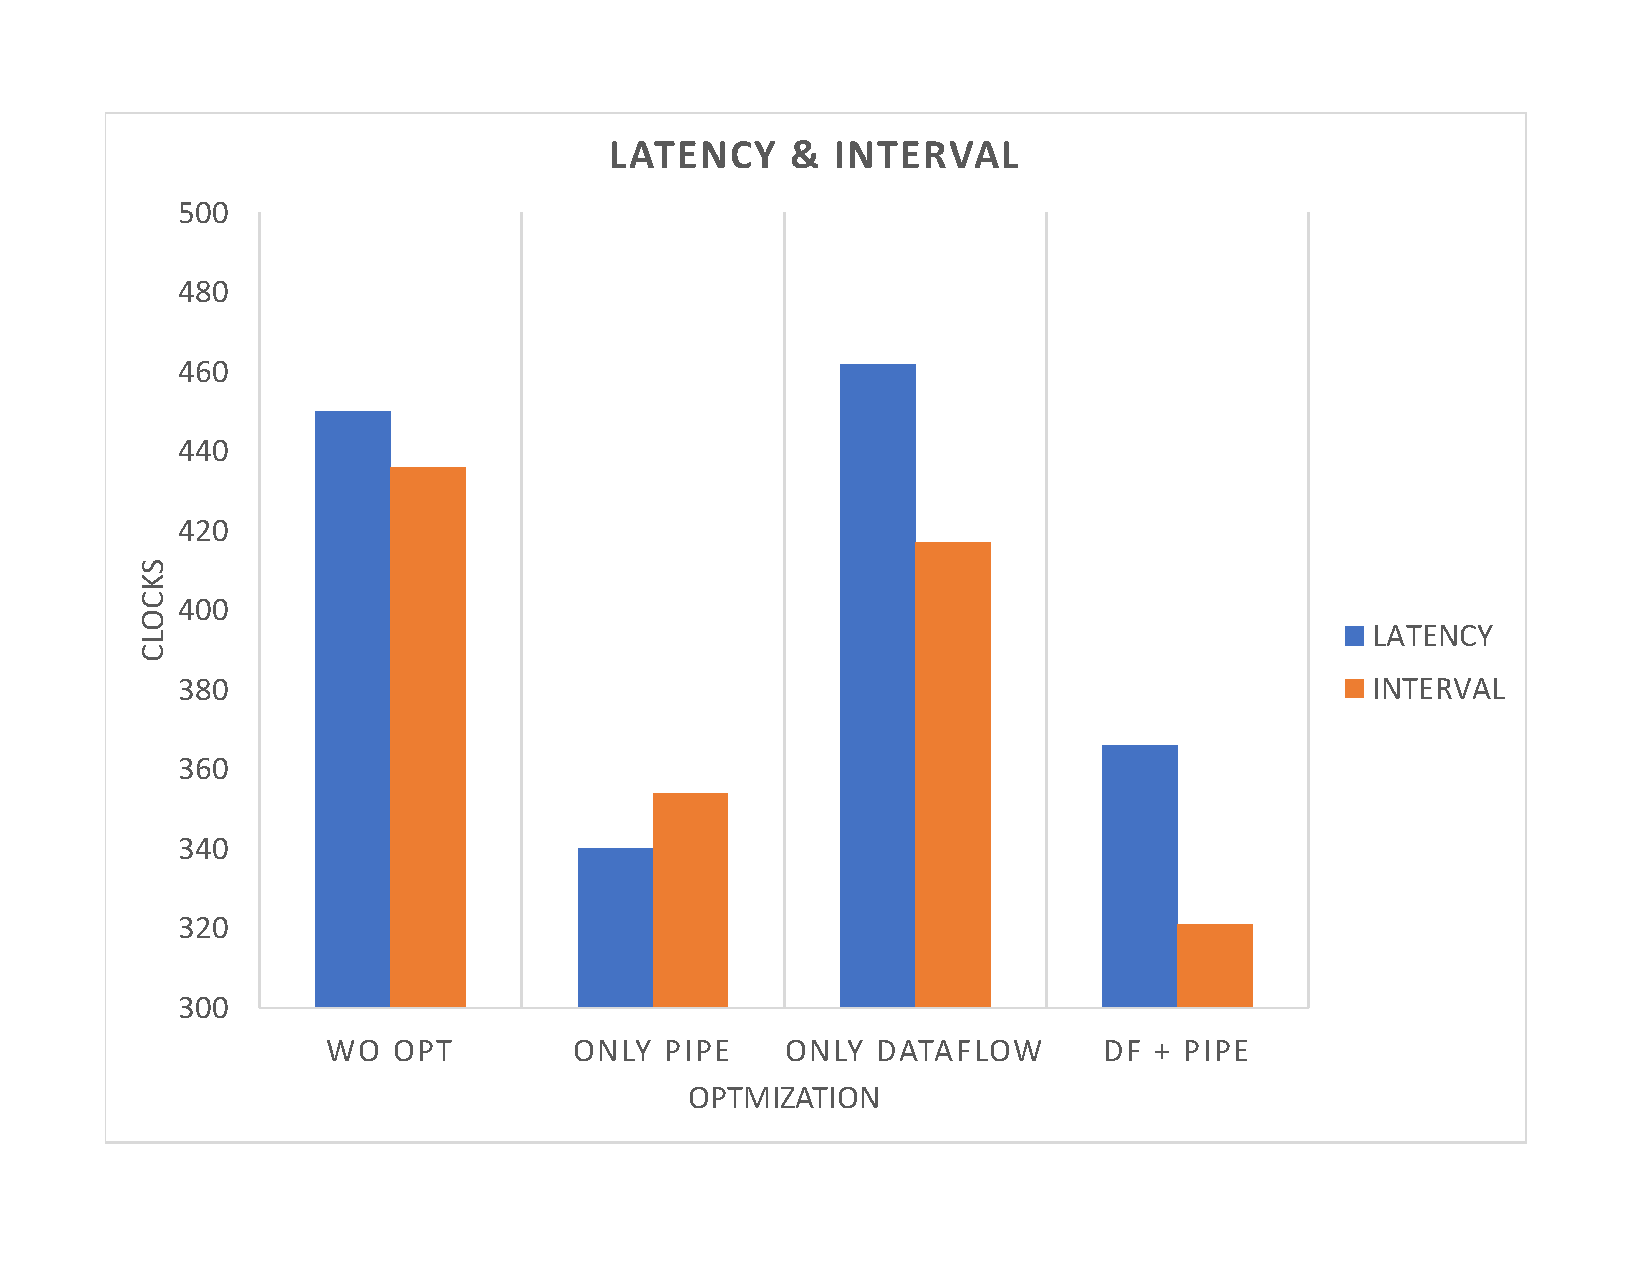
\includegraphics[scale=0.45]{Figures/LATINTFLOAT}
	\caption{Latencia e intervalo de las optimizaciones en float}
	\label{fig:latIntFloat}
\end{figure}

La Figura \ref{fig:perfGainFloat} muestra la ganancia de cada una de las optimizaciones contra la referencia (Sin optimizaciones), lo cual indica que para punto flotante, es mejor aplicar PIPELINE, obteniendo así una  reducción casi del 30\% de latencia total del circuito y 20\% más intervalo.

%tek Mirar bien los datos numéricos

\begin{figure}[!ht]
	\centering
		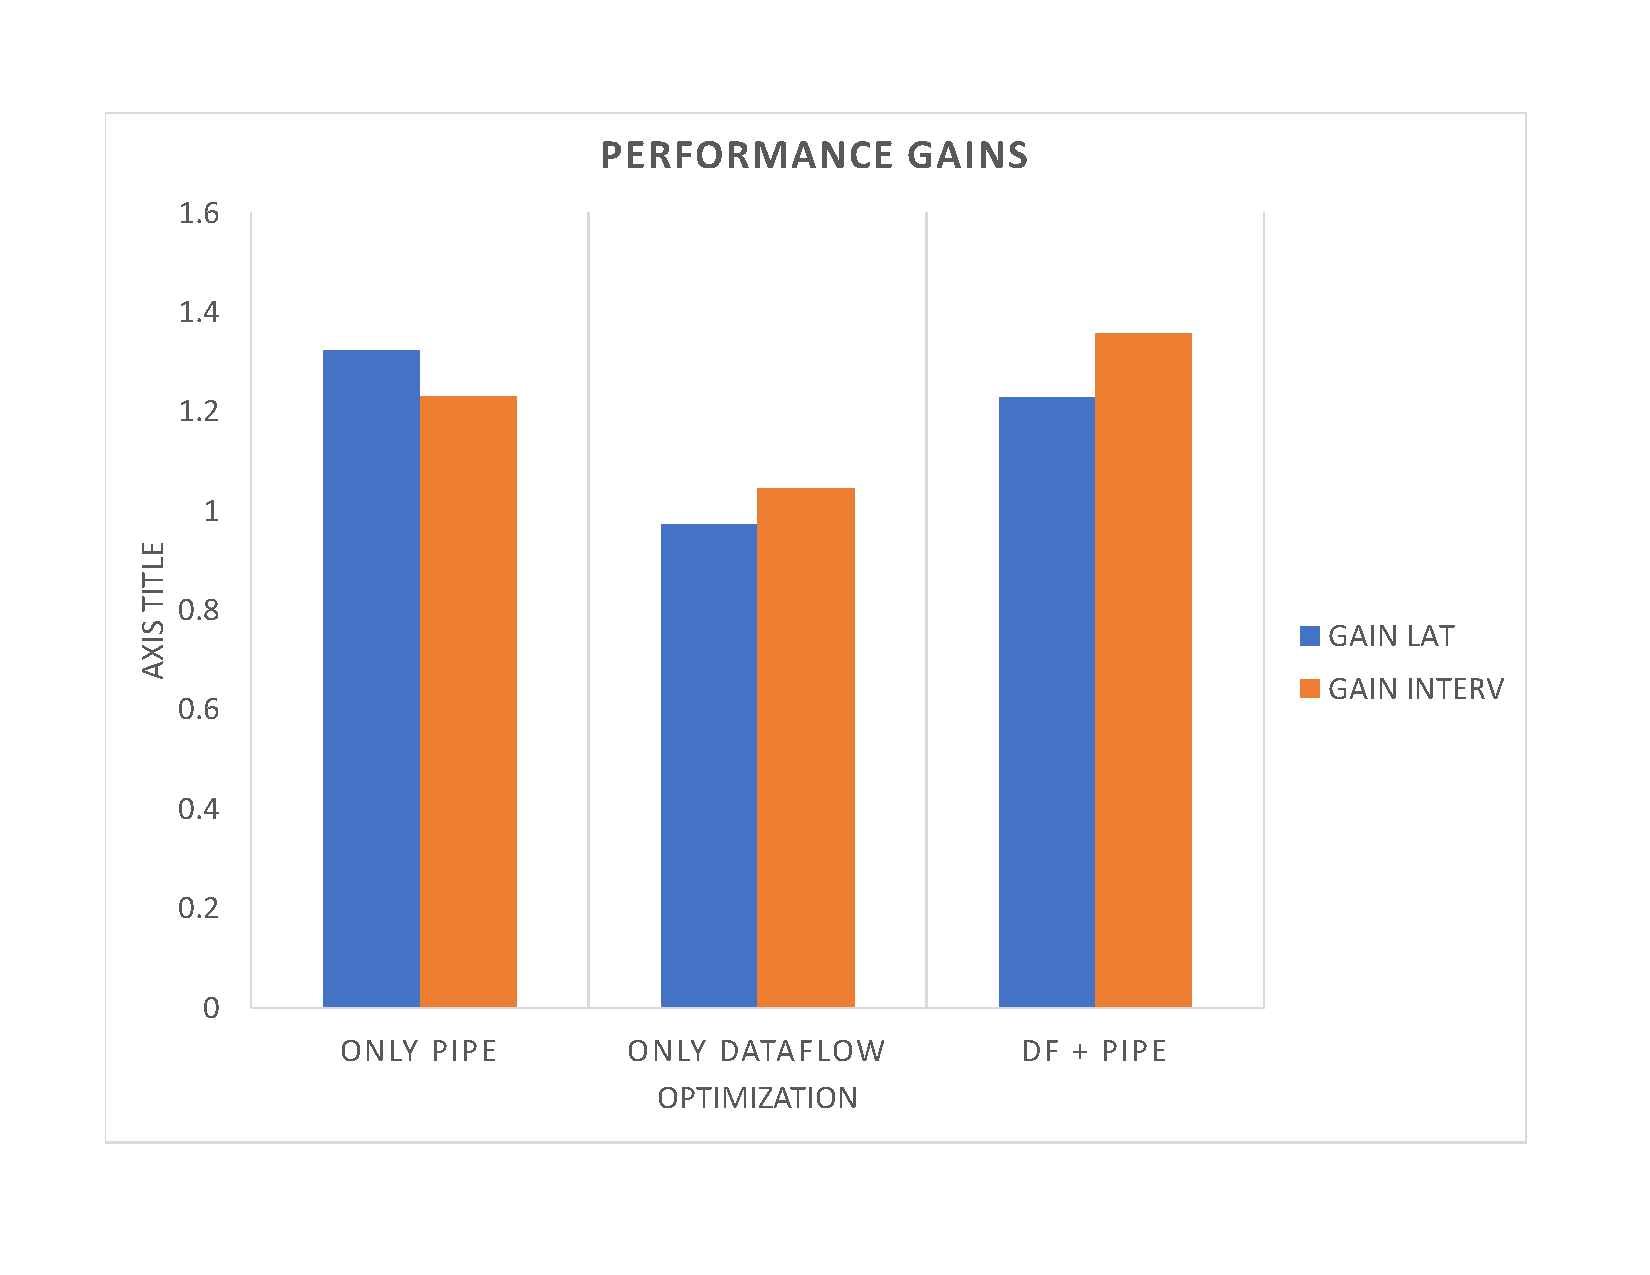
\includegraphics[scale=0.45]{Figures/PERFGAINFLOAT}
	\caption{Ganancia en rendimiento usando float}
	\label{fig:perfGainFloat}
\end{figure}

La Figura \ref{fig:latIntFix} muestra los resultados de síntesis para las mismas optimizaciones usando punto fijo.

\begin{figure}[!ht]
	\centering
		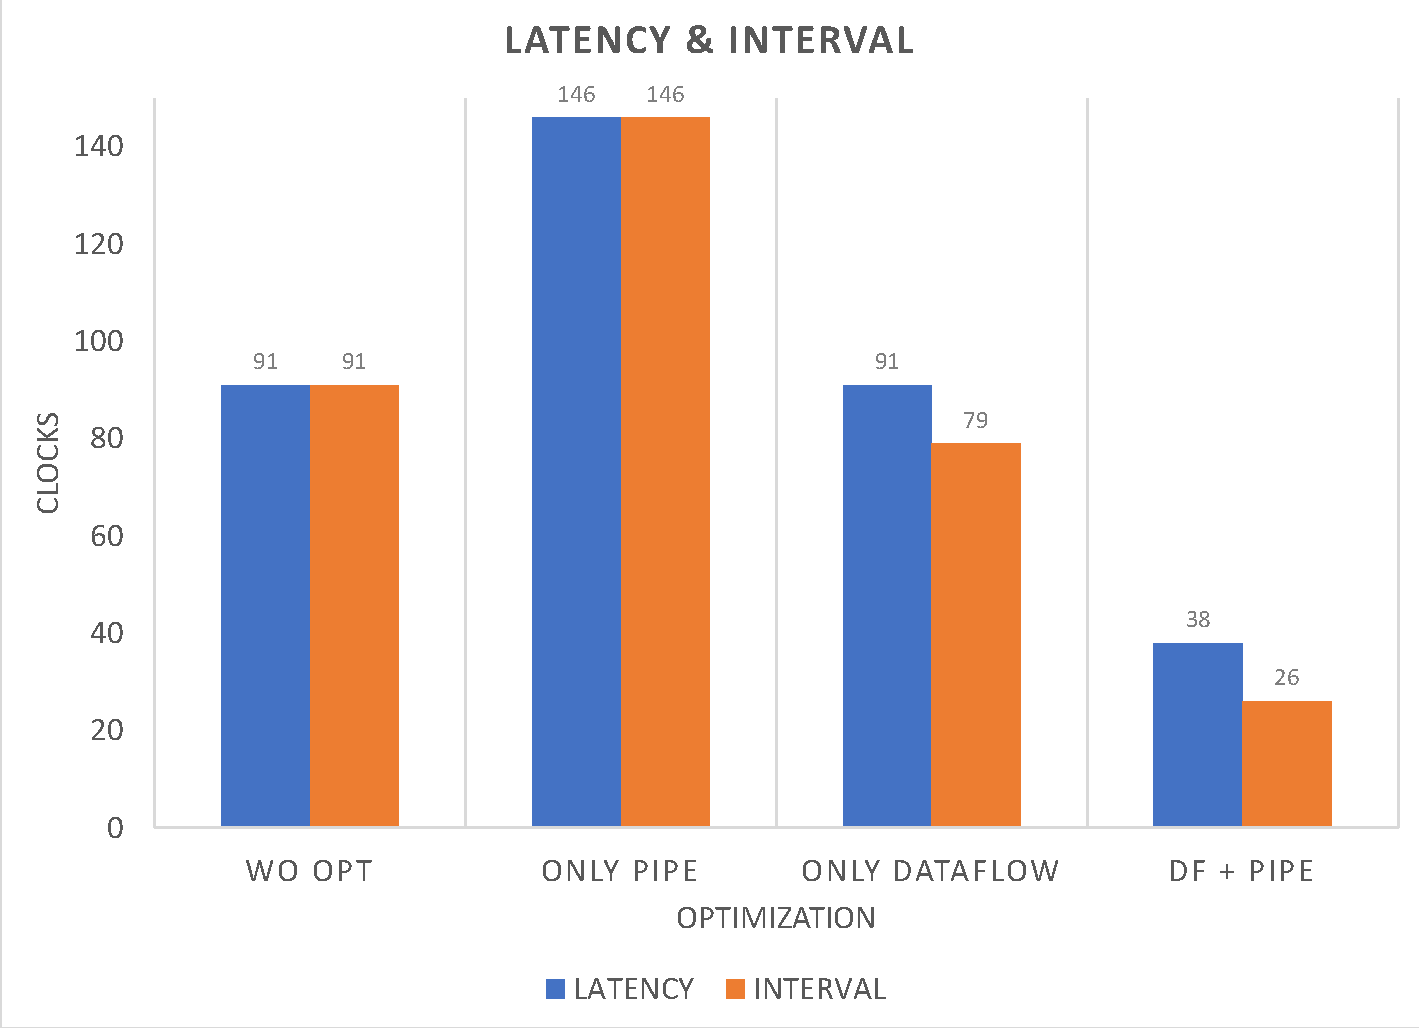
\includegraphics[scale=0.45]{Figures/LATINTFIX}
	\caption{Latencia e intervalo de las optimizaciones fijo}
	\label{fig:latIntFix}
\end{figure}

En este caso se observa un claro ganador; este puede ser corroborado por la Figura \ref{fig:perfGainFix} con 3.5 veces en mejora del intervalo y 2.5 veces de la latencia frente a la referencia.

\begin{figure}[!ht]
	\centering
		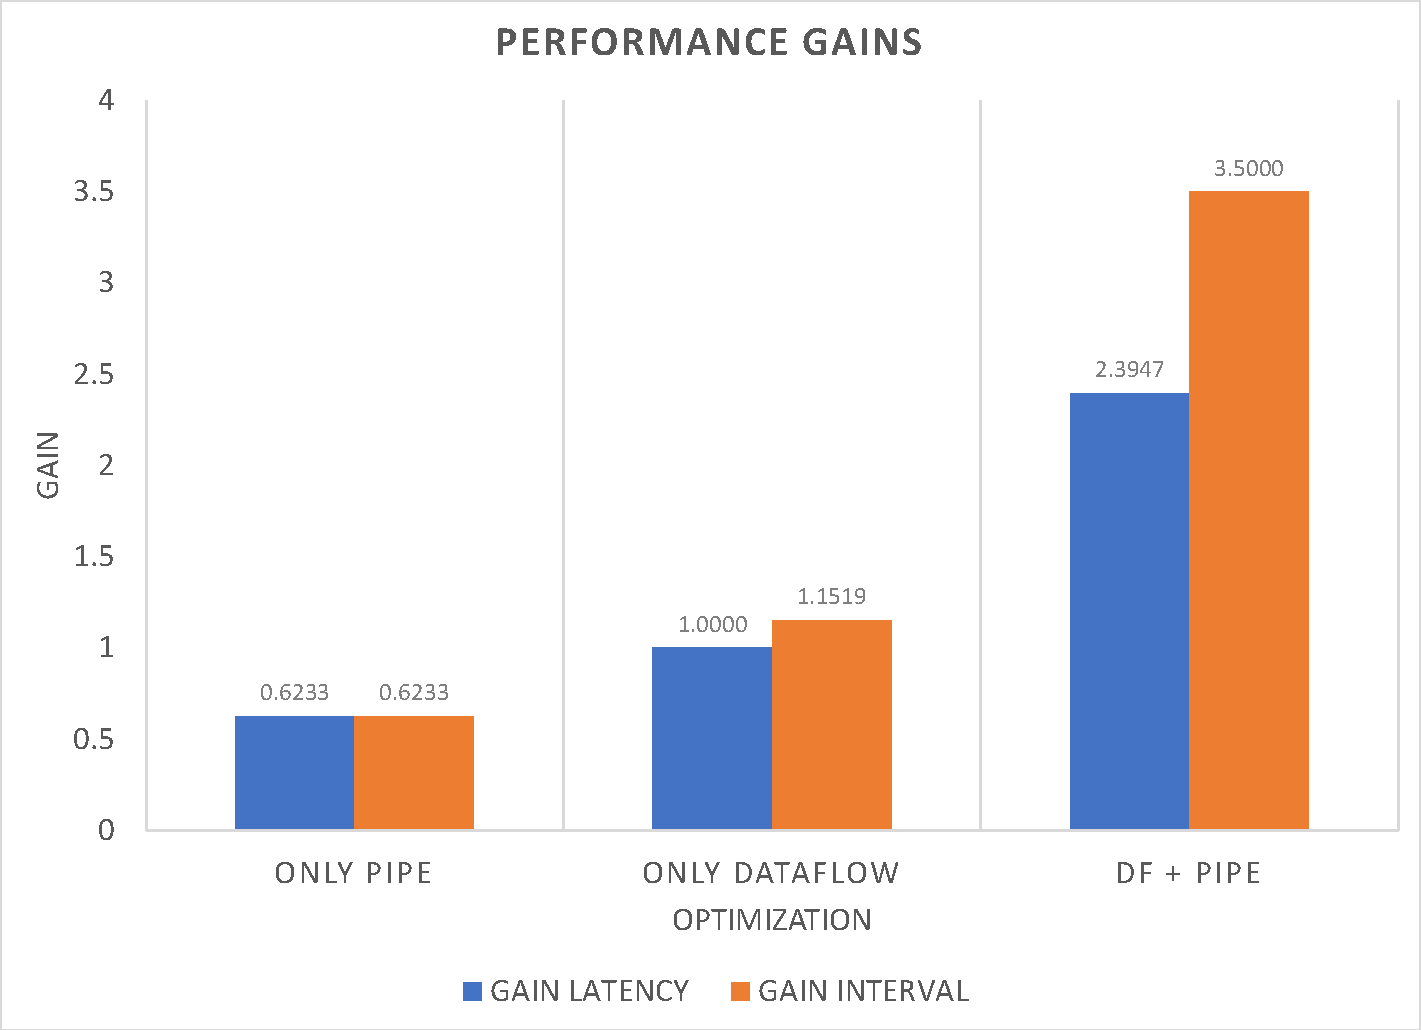
\includegraphics[scale=0.45]{Figures/PERFGAINFIX}
	\caption{Ganancia en rendimiento en float}
	\label{fig:perfGainFix}
\end{figure}

La Figura \ref{fig:fixfloat} muestra las diferencias de ganancia entre punto fijo y flotante. Es claro que las operaciones en punto fijo son menos costosas en términos de hardware; por tanto, el punto fijo y la combinación de DATAFLOW y PIPELINE son la combinación de optimizaciones a sintetizar e implementar en hardware.

\begin{figure}[!ht]
	\centering
		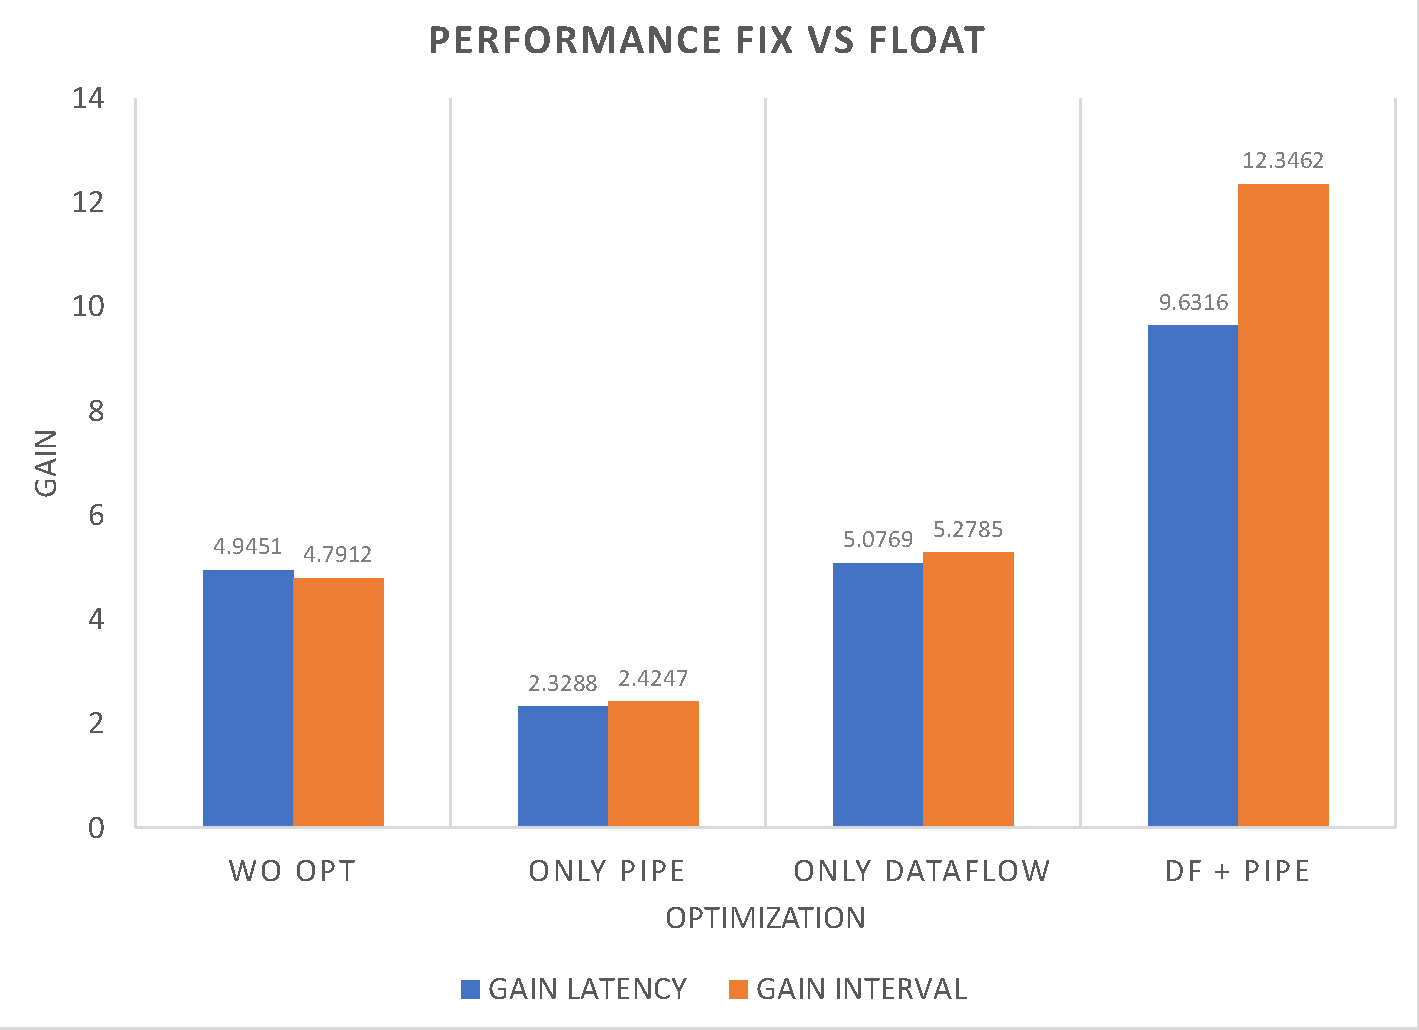
\includegraphics[scale=0.45]{Figures/fixfloat}
	\caption{Diferencia entre punto fijo y flotante}
	\label{fig:fixfloat}
\end{figure}

\subsection{Implementación del hardware}

En esta sub sección se hablará de la implementación de hardware usando el sintetizador de hardware Vivado. La Figura \ref{fig:hwImp} muestra la implementación final. En ella se observan 3 conectores AXI en el módulo \textbf{TOPANN\_0}; los de la derecha representan los maestros AXI HP, encargados de iniciar las transacciones de datos desde y hacia la memoria RAM con sus respectivos Bursts; el conector AXI Lite a la izquierda del módulo corresponde al esclavo encargado de recibir los datos de los pesos desde la memoria RAM. Se determinó que era la mejor implementación, dado que los AXI HP otorgan un ancho de banda más amplio en tanto que los pesos de la red que no cambian en el tiempo, se pueden trabajar con un puerto AXI Lite.

\begin{figure}[!ht]
	\centering
		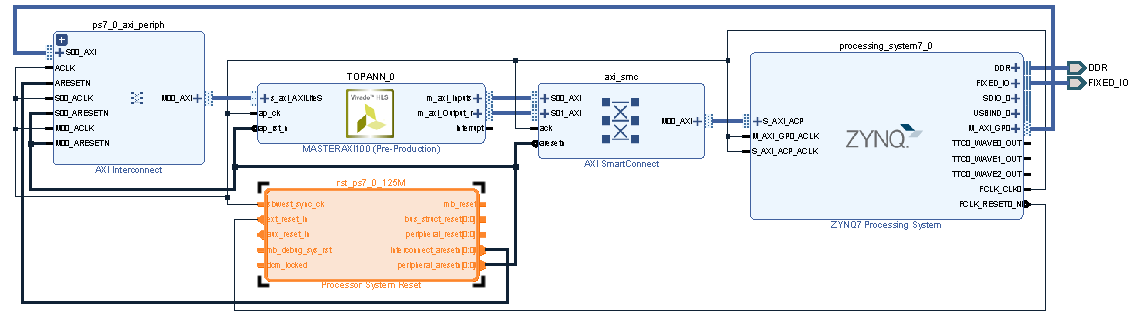
\includegraphics[scale=0.95]{Figures/hwImp}
	\caption{Implementación final de hardware}
	\label{fig:hwImp}
\end{figure} 

La Tabla \ref{tab:resourcesPostSynt} enseña la cantidad de recursos de la FPGA usados por la implementación propuesta una vez ha sido sintetizado el hardware necesario. En ella, se muestra en porcentaje usado del hardware disponible de la tarjeta de desarrollo el consumo de cada una de las unidades lógicas y de procesamiento de la FPGA por cada una de las optimizaciones propuestas. Se observa que la implementación de \textbf{DATAFLOW} más \textbf{PIPELINE} escogida para ser implementada es la que presenta mayor uso de recursos. Esto se debe al alto nivel de concurrencia que ocurre a nivel de las tareas y los buclues, otorgando un paralelismo máximo. Las implementaciones de \textbf{DATAFLOW}, \textbf{PIPE UNROLL}, y \textbf{NO OPT} son similares en cuanto a uso de hardware y su diferencia debería ser notable en tiempo de ejecución. Finalmente, en búsqueda de un equilibrio entre los recursos y el rendimiento del bloque, se configuró el sintetizador en modo de optimización de área; esto lo que garantiza es que se reutilicen los recursos de hardware disponibles de tal modo que se use la menor cantidad para implementar el circuito. En este escenario, se observa que la síntesis con optimización de área otorga una reducción de aproximadamente el 50\% en promedio de los recursos totales utilizados frente a la solución numéricamente más deseable.

%tek Revisar redacción

\begin{table}[h!]
\centering
\begin{tabular}{|c|c|c|c|c|c|c|}
\hline
 & LUT\% & \begin{tabular}[c]{@{}c@{}}LUT\\ RAM\% \end{tabular} & FF\% & BRAM\% & DSP\% & AVERAGE\% \\ \hline
\begin{tabular}[c]{@{}c@{}}DF PIPE\\ AREA OPT\end{tabular} & 27 & 12 & 15 & 13 & 15 & 16.4 \\ \hline
\begin{tabular}[c]{@{}c@{}}DF \\ PIPE\end{tabular} & 53 & 22 & 25 & 35 & 35 & 34 \\ \hline
\begin{tabular}[c]{@{}c@{}}DATA\\ FLOW\end{tabular} & 38 & 24 & 19 & 13 & 15 & 21.8 \\ \hline
\begin{tabular}[c]{@{}c@{}}PIPE\\ UNROLL\end{tabular} & 38 & 23 & 21 & 15 & 20 & 23.4 \\ \hline
\begin{tabular}[c]{@{}c@{}}NO\\ OPT\end{tabular} & 37 & 23 & 19 & 13 & 15 & 21.4 \\ \hline
\end{tabular}
\caption{Tabla uso de recursos post síntesis}
\label{tab:resourcesPostSynt}
\end{table}



%tek más óptima?

Con esto se tiene un conjunto de pruebas de cuatro circuitos diferentes para ser analizados en la plataforma de pruebas.

\section{Diseño de Software}
El diseño consta de múltiples partes. Una de ellas es el diseño de la ANN como tal; el diseño de hardware y optimizaciones a implementar; y, el esquema de reconfiguración dinámico basado en el contexto de ejecución, en este caso el estado o riesgo de inundación que pueda tener el río en un momento determinado. En esta sección se analizarán los criterios para el diseño del software; en este caso, es la capa que interconecta el hardware diseñado en la sección anterior con el procesador principal ARM A9, usando como medio el kernel de Linux.

En este caso, el diseño del software implica conocer sobre el user space driver del kernel de Linux, que implica mapear las direcciones físicas de memoria entregadas por el módulo IP implementado en la FPGA a un espacio de memoria virtual manejado por el kernel.

La Figura \ref{fig:userSpaceDriver} muestra la mecánica de un driver funcionando bajo un esquema de espacio de usuario: el dispositivo hardware, en este caso ``Device'', recibe y escribe la información que necesita bajo una dirección física de memoria. El usuario, para acceder a esas direcciones de memoria, debe conocer la dirección base física a la cual el dispositivo está accediendo, el cual es provisto por el diseñador del hardware o en este caso el sintetizador HLS y el tamaño de paginación de memoria que entrega el SO. Con esto, el driver puede mapear la dirección de memoria a una virtual a la cual la aplicación pueda acceder como una referencia de memoria; en el caso de C/C++, como un apuntador que puede ser manipulado según sea necesario.

\begin{figure}[!ht]
	\centering
		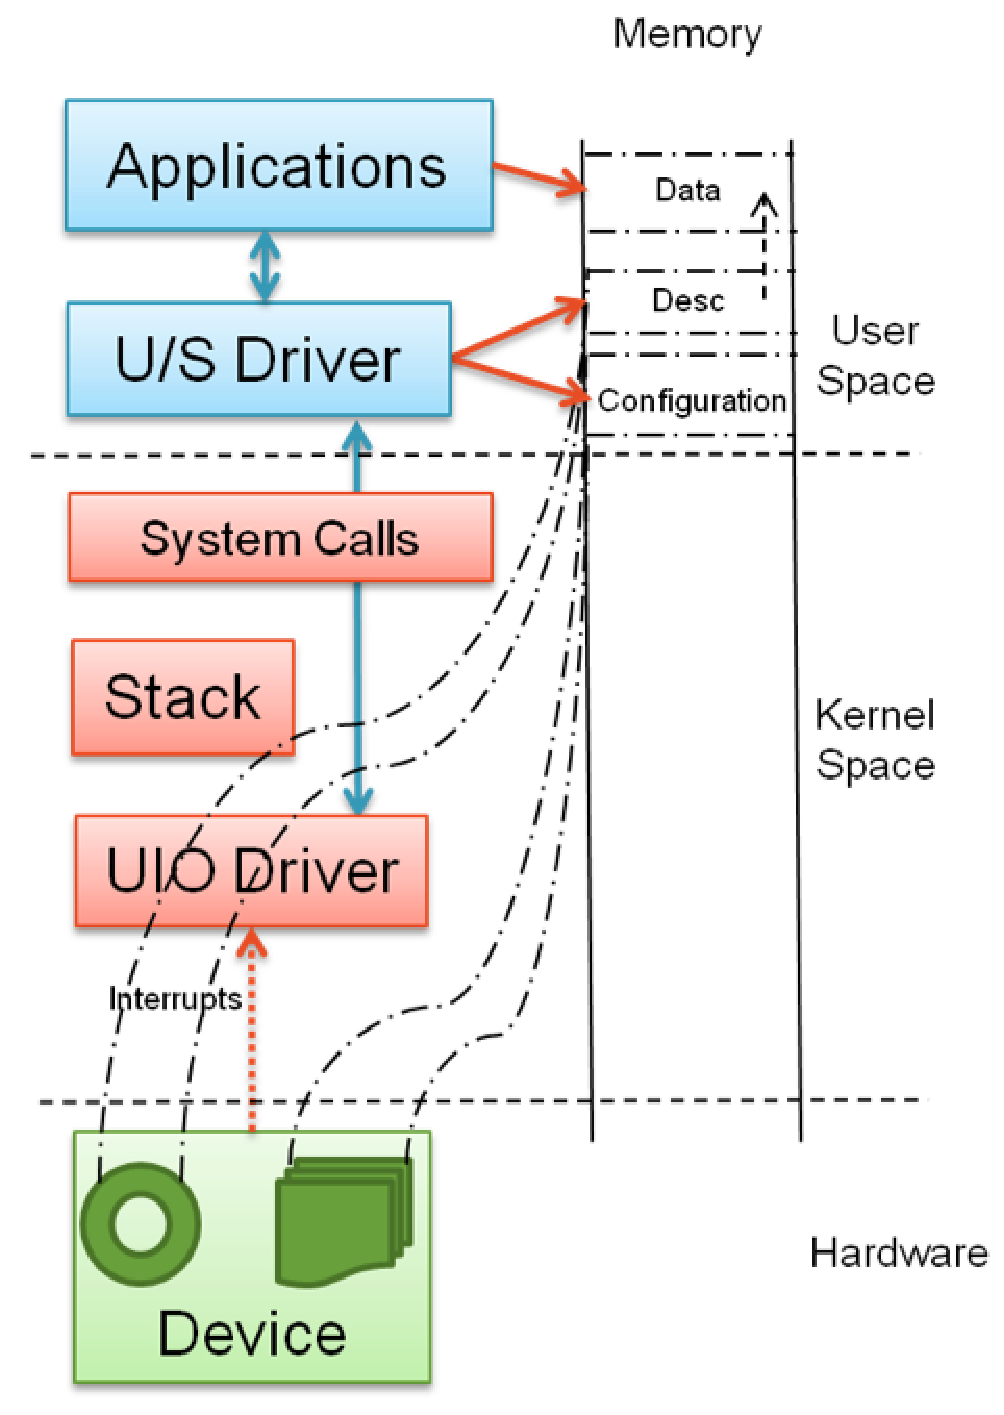
\includegraphics[scale=0.5]{Figures/UserSpaceDriver}
	\caption{Esquema de driver en espacio de usuario\cite{userSpaceDriver}.}
	\label{fig:userSpaceDriver}
\end{figure}

\subsection{Petalinux SDK}

Petalinux es una distribución especial del proyecto Yocto \citep{Yocto}, cuya razón de existir es ayudar a los desarrolladores a crear sus propias distribuciones del kernel de Linux para dispositivos embebidos. Xilinx desarrolló su propia versión del kernel basado en Yocto llamándolo Petalinux y su conjunto de herramientas conocidas como Petalinux SDK. Petalinux SDK cuenta con un gran conjunto de herramientas de compilación y ayudas al desarrollador para simplificar el proceso de personalizar y compilar el kernel de Linux para ser distribuido dentro de una de las tarjetas de desarrollo de Xilinx.

Para que un bloque IP funcione dentro de un chip ZYNQ de Xilinx debe cumplir varios requisitos.

\begin{itemize}
\item La FPGA debe ser configurada por el JTAG o por el PS7.
\item Los registros de memoria y del procesador deben ser fijados usando el procedimiento estándar de arranque descrito en la Figura \ref{fig:arranqueFPGA}.
\item Si se requiere una implementación con el kernel Petalinux, se debe garantizar que el kernel sea compilado usando Petalinux SDK con el DeviceTree y el Board Support Package (bitstream incluido) creado usando la herramienta de síntesis Vivado.
\item Se debe inicializar el bloque IP usando los registros otorgados por la herramienta de síntesis de alto nivel Vivado HLS.
\end{itemize}

\begin{figure}[H]
	\centering
		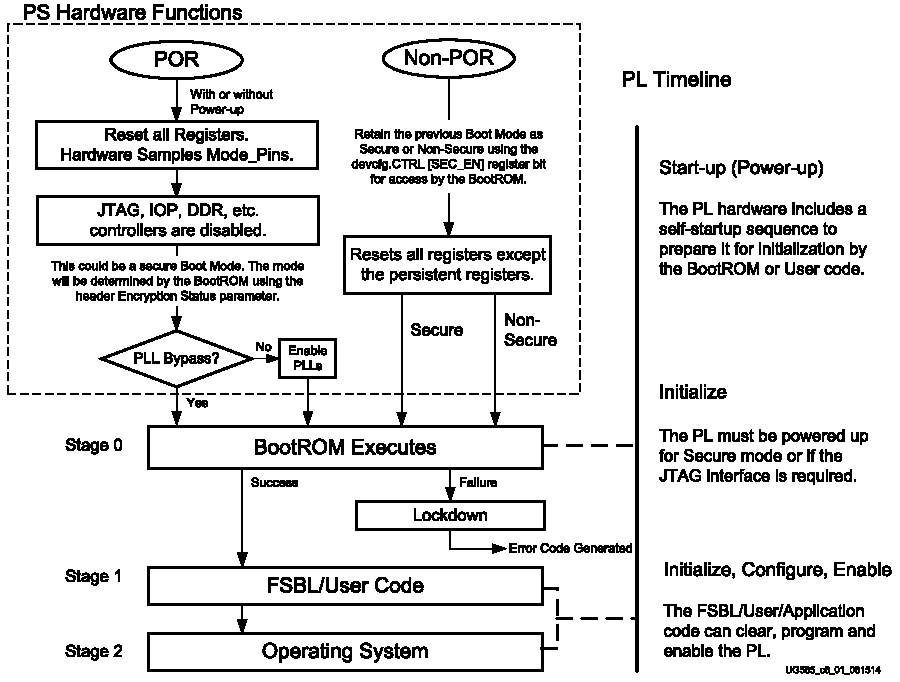
\includegraphics[scale=0.8]{./Figures/I3.pdf}
	\caption{Estructura de arranque de sistemas ZYNQ \citep{TRM2017}}
	\label{fig:arranqueFPGA}
\end{figure}

\subsubsection{Configuración de Petalinux SDK}

Dado el volumen de datos y la posibilidad de cambiar el software en línea sin recompilar el kernel de Linux se decidió que la solución debería contar con las siguientes características:

\begin{itemize}
\item Persistencia de los datos.
\item Conexión de red Ethernet.
\item Conexión serial a 115200 baudios.
\item Ejecutar software usando el User Space de Linux.
\end{itemize}

Para cumplir con lo anterior, se configura el kernel de Linux de la siguiente forma:

\begin{verbatim}
// usando bash de Linux
petalinux-config
// Una vez en el menú configurar de la siguiente manera
Image Package Configuration -> Root File System Type -> SD Card
// Salvar los cambios y salir del menú

// Usando bash de Linux
petalinux-config -c kernel
//Configurar de la siguiente manera
Device Drivers -> 
<*>User I/O platform driver with generiq IRQ handling
<*>User Platform Driver with generiq irq and dynamic memory
// Salvar y salir del menú
\end{verbatim}

Se debe garantizar la configuración del Device Tree Blob de la siguiente manera:

\begin{verbatim}
// Válido para Petalinux SDK 2017.4 y compatibles
// Modificar el archivo system-user.dtsi
// Ubicación: ./carpeta-proyecto/projec-spec/meta-user/recipes-bsp/device-tree/files

/include/ "system-conf.dtsi"
/ {

	chosen {
		bootargs = "console=ttyPS0,115200 earlyprintk uio_pdrv_genirq.of_id=generic-uio
        root=/dev/mmcblk0p2 rw rootwait";
	};

};

&TOPANN_0  {
			compatible = "generic-uio";
			reg = <0x43c00000 0x10000>;
			xlnx,s-axi-axilites-addr-width = <0x8>;
			xlnx,s-axi-axilites-data-width = <0x20>;
		};

&gem0 {
	phy-handle = <&ethernet_phy>;
/*	phy-reset-gpio = <&axi_gpio_eth 0 0>;
	phy-reset-active-low;	
	phy-reset-duration = <10>; */
	ethernet_phy: ethernet-phy@1 { /* rtl8211e-vl */
		reg = <1>;
		device_type = "ethernet-phy";
	};
};
\end{verbatim}

De esta forma, con las configuraciones dadas anteriormente, es posible compilar el kernel de Linux y con el driver adecuado debería ser posible que el hardware funcione dentro de la FPGA y sea controlado desde Petalinux.

\subsection{Diseño del driver}
Para el driver se tomó la decisión de usar el lenguaje C++ dado que permite el uso del paradigma de programación orientada a objetos, el cual permite crear diferentes módulos con funcionalidad determinada que luego pueden ser heredados a otros objetos para mejorar o ampliar el funcionamiento de los mismos. En este caso, se usaron diferentes clases u objetos que permitirían al desarrollador mapear la memoria, inicializar el módulo de aceleración de hardware con las secuencias de bits requeridos por la interfaz AXI y la operación del módulo de como tal, es decir la carga de los pesos de la ANN, los datos a procesar y los resultados de la operación.

%tek Revisar redacción

La implementación del driver se ve en la Figura \ref{fig:userSpaceDriverModel}. En ella se resumieron los métodos usados para mapear la memoria y manipular los datos que llegan y van hacia el módulo acelerador en la FPGA. La clase \texttt{ANNService} recibe como dependencia las direcciones de memoria mapeadas en la clase \texttt{Driver} mediante la clase \texttt{Controller}. La clase \texttt{ANNService} a su vez, usa la clase \texttt{ANN\_DAO}, que recibe como dependencia, una estructura de almacenamiento desacoplando la aplicación del método de persistencia. En este caso, dado que se busca obtener el performance de la aplicación como tal, se usó persistencia en memoria.

\begin{figure}[!ht]
	\centering
		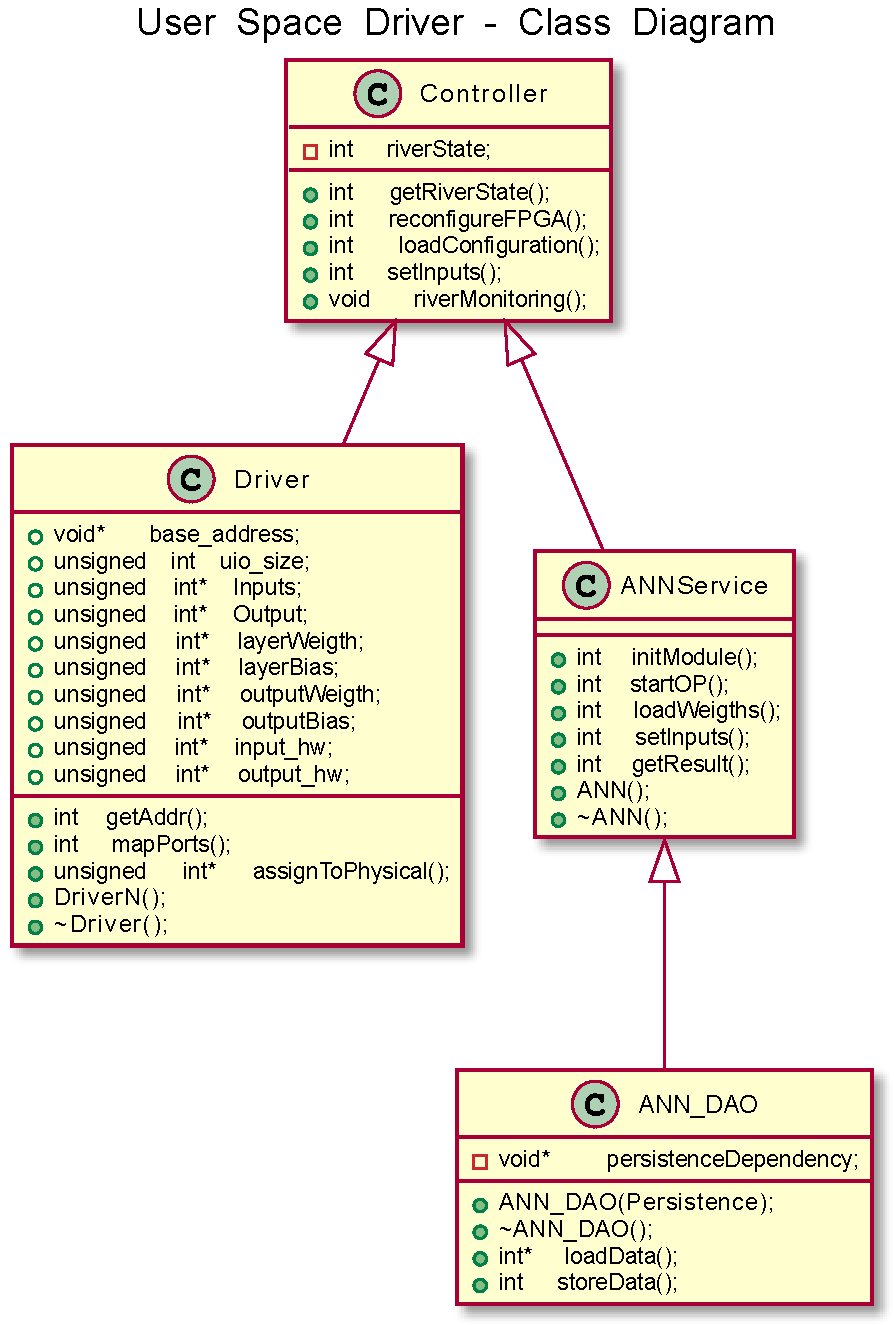
\includegraphics[scale=0.8]{Figures/driverANN}
	\caption{Diagrama de clases de la aplicación}
	\label{fig:userSpaceDriverModel}
\end{figure}

\subsection{Diseño del controlador de reconfiguración}

Teniendo en cuenta que se requiere que el controlador monitoree el estado del río mediante el estado de la ANN, se optó por un diseño reactivo del controlador, donde el riesgo de inundación disparado por la ANN activa los mecanismos de reconfiguración, la velocidad de muestreo y la recepción de datos proveniente de los nodos aledaños.

La Figura \ref{fig:esquemaFuncionamiento} muestra cómo estaría configurada la FPGA en su modo lazy o flojo, pudiendo atender los datos provenientes de los nodos aledaños cuando el Controlador detecta un riesgo de inundación; es decir que, la salida de la red ``ANN 1'' sobrepasa el umbral de entre 70\% y 80\%. Cuando el PS detecta una salida de la ``ANN 1'' sobre ese umbral, el procesador reconfigura automáticamente la FPGA para recibir un mayor número de entradas provenientes de campo. Dado que es el mismo circuito, todos estos datos pasarían por la misma interfaz AXI High Performance.

\begin{figure}[!ht]
	\centering
		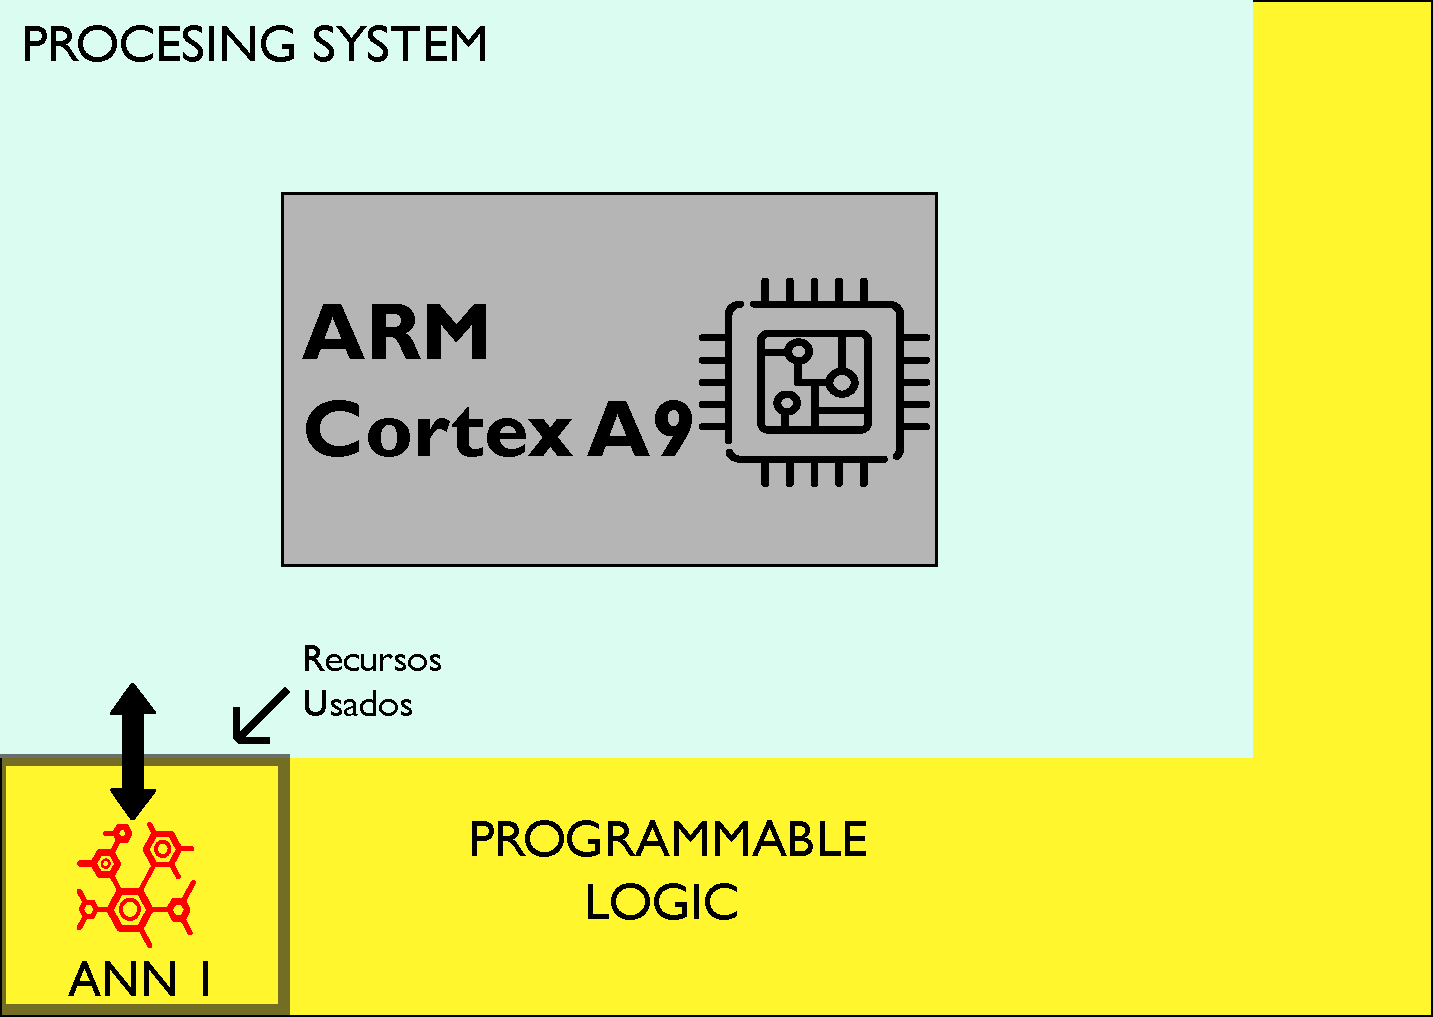
\includegraphics[scale=0.5]{Figures/ANN1}
	\caption{Esquema de funcionamiento ANN}
	\label{fig:esquemaFuncionamiento}
\end{figure}

Al reconfigurar el circuito se espera que la cantidad de área asignada al circuito cambie. En este caso, la variación está dada en función de las entradas a analizar (Neuronas de Entrada), pues se incrementa la cantidad de Look Up Tables y Block RAMs necesarias para operar la ANN.

Esto aplica también para configuraciones o aplicaciones en las que dinámicamente se adiciona hardware; la diferencia con la Figura \ref{fig:esquemaFuncionamientoReconfig}, es que se crean y se usan nuevas interfaces AXI HP que se unen al bus AMBA.

\begin{figure}[!ht]
	\centering
		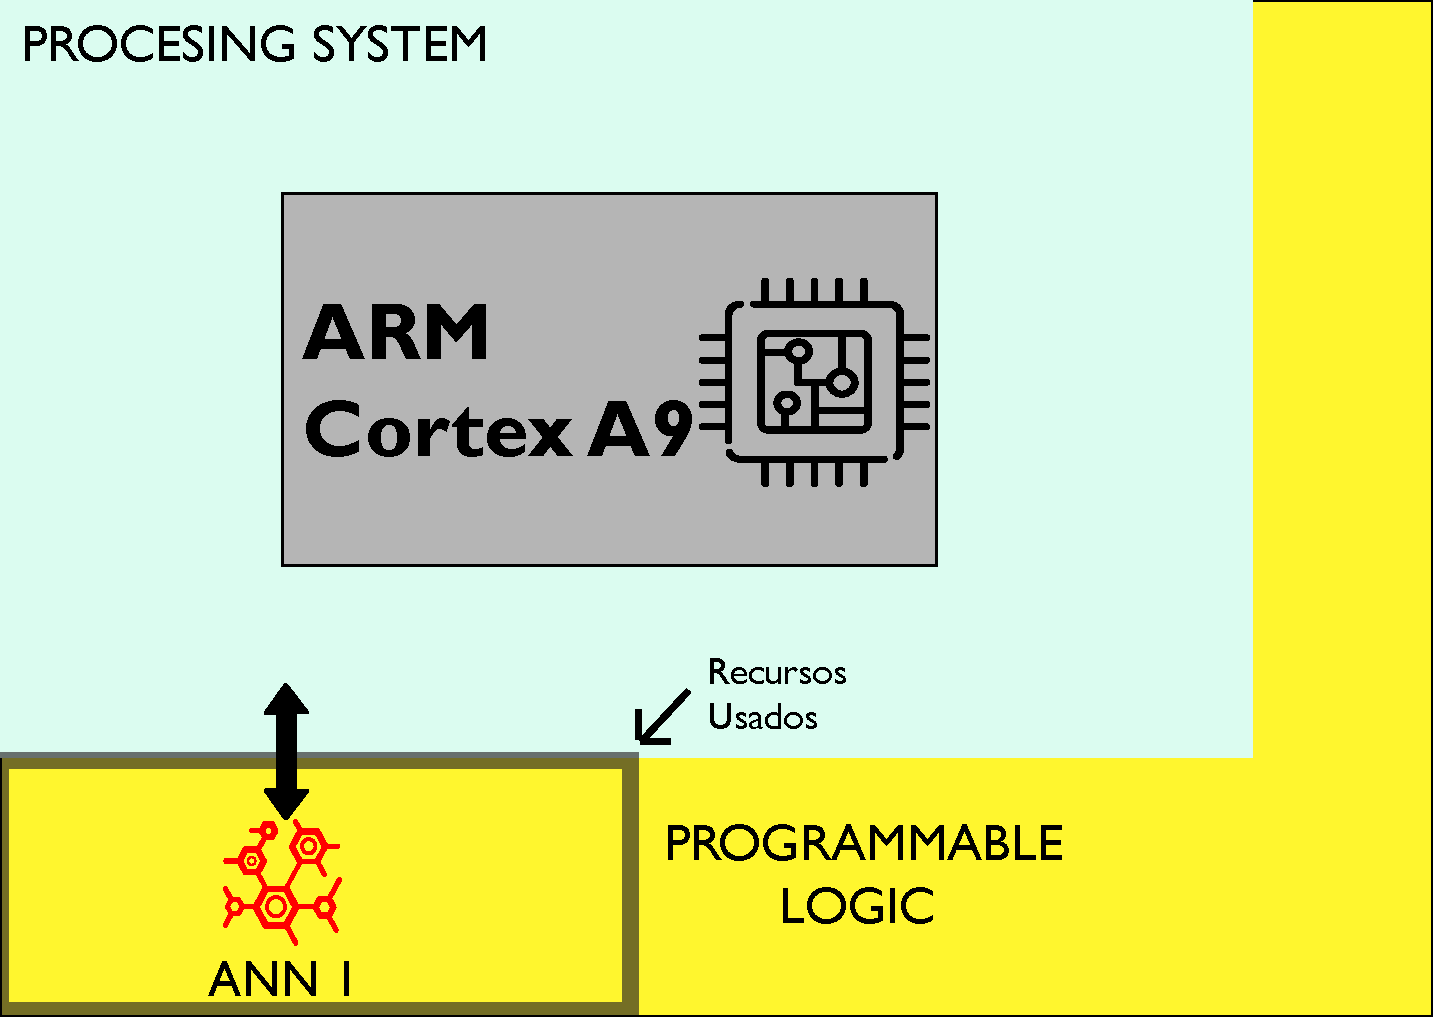
\includegraphics[scale=0.5]{Figures/ANN2}
	\caption{Esquema de funcionamiento ANN reconfigurada}
	\label{fig:esquemaFuncionamientoReconfig}
\end{figure}

La Figura \ref{fig:esquemaFuncionamientoReconfig2} muestra un esquema de configuración para múltiples aplicaciones ejecutándose en la FPGA de forma concurrente. Cada una de las instancias de las aplicaciones posee su propia interfaz AXI otorgando acceso directo a la RAM, por lo que cada una podría realizar actividades diferentes y la única actividad que debería realizar el controlador es alimentar y monitorear as direcciones de memoria correspondientes a cada uno de los bloques.

\begin{figure}[!ht]
	\centering
		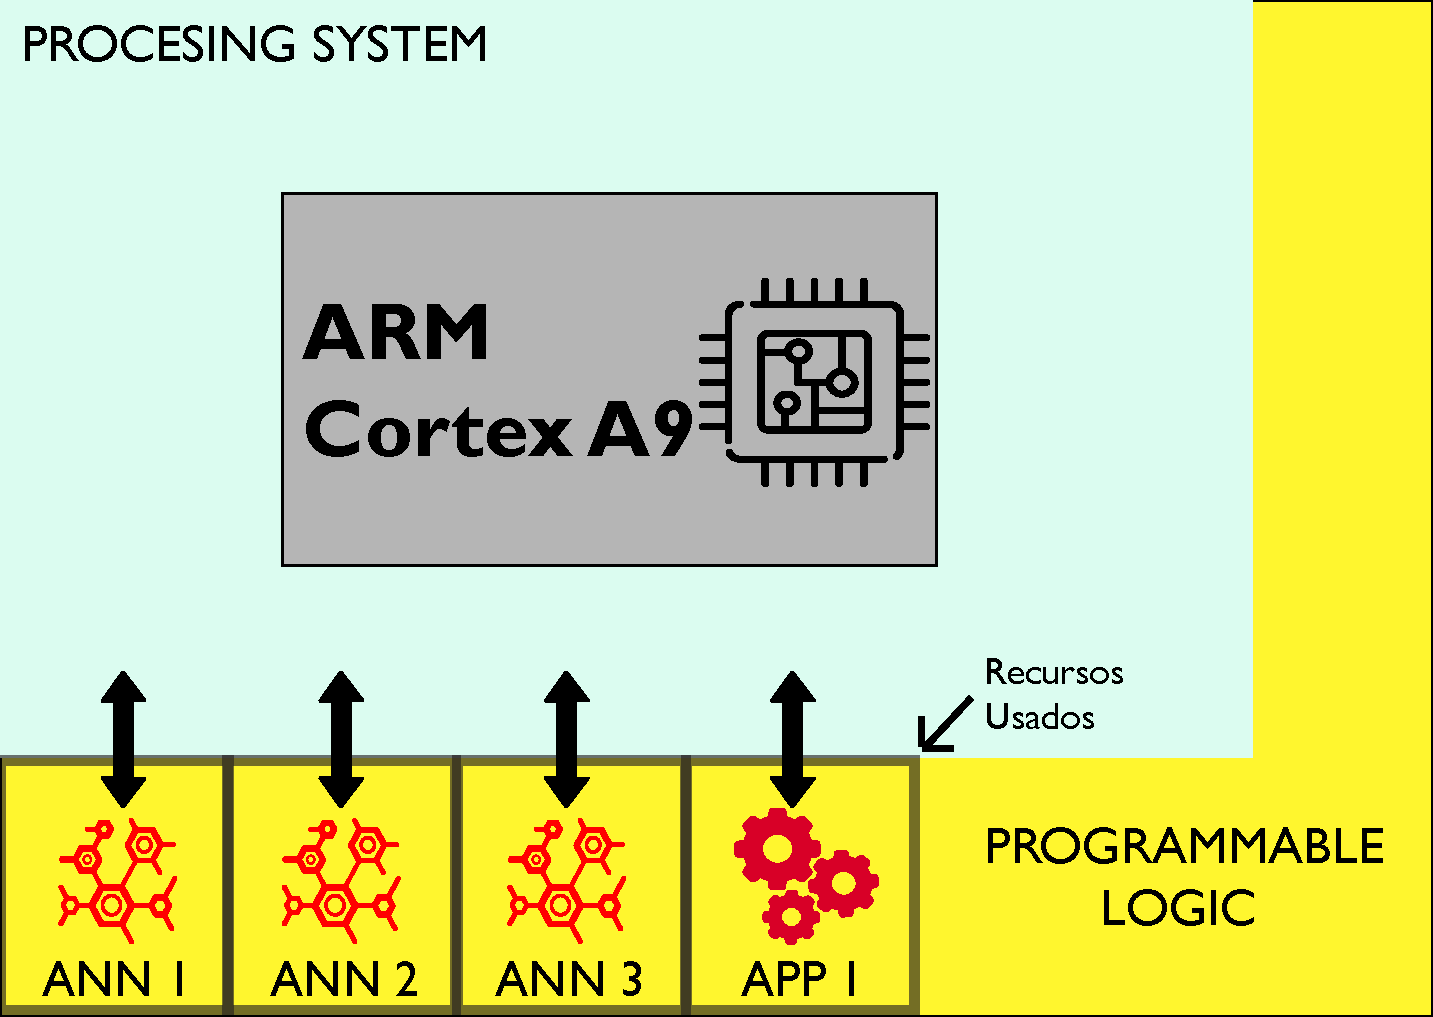
\includegraphics[scale=0.5]{Figures/ANN3}
	\caption{Esquema de funcionamiento múltiples aplicaciones}
	\label{fig:esquemaFuncionamientoReconfig2}
\end{figure}
 %Diseño HW/SW

% Chapter 11

\chapter{Comparación Modelo de la ANN} % Write in your own chapter title
\label{Chapter12}
\lhead{Capítulo 12. \emph{Comparación ANN}} % Write in your own chapter

En este capítulo se analizará comparativamente los niveles de detección entre un modelo de Red Neuronal Artificial usando las herramientas de Matlab (nntool) y el modelo en hardware propuesto en este documento en el Capítulo \ref{Chapter6}, figura \ref{fig:MLP}. El objetivo es demostrar que el modelo propuesto es válido y puede ser implementado a nivel de hardware directamente. Para esto se eligió mostrar la detección del modelo de la red en punto fijo usando el entrenamiento de Matlab con especificaciones iguales a las del modelo Hardware propuesto, por otra parte se usó el entrenamiento directamente sobre el modelo hardware usando C/C++.

\begin{figure}[H]
	\centering
		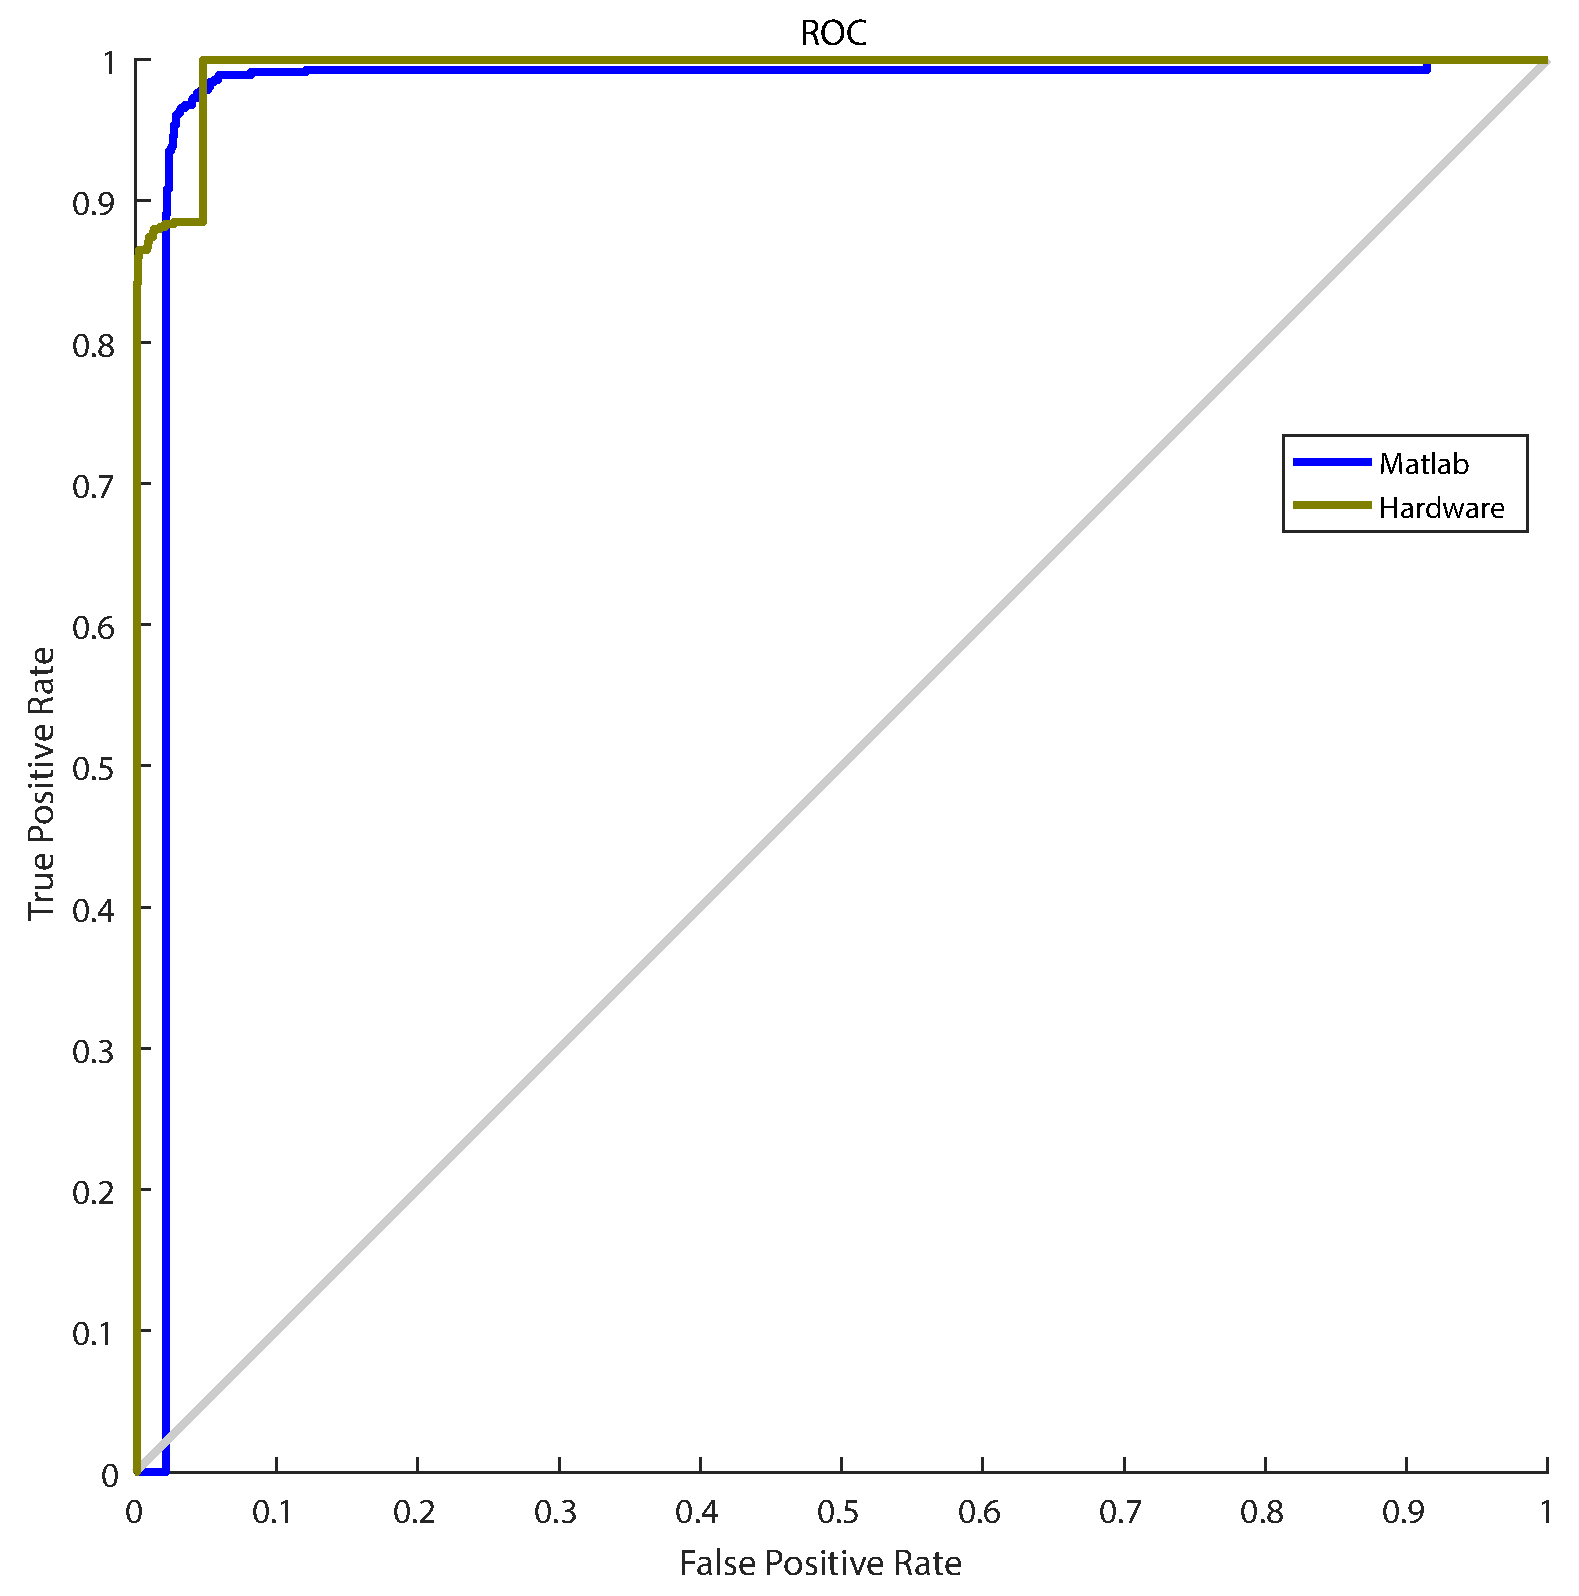
\includegraphics[scale=0.35]{./Figures/ROCANN}
	\caption{Curva ROC de detección}
	\label{fig:ROC}
\end{figure}

 La Figura \ref{fig:ROC} muestra la curva ROC o Receiver Operating Characteristic por sus siglas en inglés, esta gráfica lo que muestra es la calidad del clasificador al discriminar entre un valor de detección positivo y otro negativo basado en el conjunto de datos de entrenamiento. Particularmente una curva ROC muestra lo siguiente según su forma \citep{ROCCurve}:
 
 \begin{itemize}
     \item Se muestra el balance entre la sensibilidad (eje vertical) y la especificidad (eje horizontal), donde un incremento en la sensibilidad va acompañado de un detrimento de la especificadad.
     \item Entre más cerca la curva esté al eje vertical izquierdo y al eje horizontal superior más efectivo es el clasificador.
     \item Entre más cerca esté la curva a la diagonal menos efectivo es el clasificador.
 \end{itemize}
 
 En esta gráfica lo que vemos es que el clasificador tanto en software como en hardware funciona pero debido al entrenamiento presenta algunas detecciones falsas, esto mayoritariamente se debe a las fluctuaciones generadas por el transitorio entre los estados de inundación y sequía propios del conjunto de datos, generando falsos positivos y/o negativos. Esto es posible corregirlo ajustando los parámetros del entrenamiento a tal punto que las fluctuaciones en la detección sean menos notorias, pero particularmente para este problema las transiciones seguirán presentes. Corregir los estados de detección erroneo causados por el entrenamiento y conjunto de datos puede ser corregido ajustando la salida de la RNA con un circuito de retraso que pueda interpretar los rápidos cambios de estado, suavizando la salida de la RNA de tal forma que no se vea afectada la medición final.


Tras analizar ambas redes como clasificador, se hace necesario analizar punto a punto la señal con tal de determinar que efectivamente ambos modelos están entregando punto a punto una equivalencia para el conjunto de datos entregado. Para ello se eligió calcular el indice de correlación y la correlación cruzada. En el primer caso, el índice de correlación es de $0.9329$, siendo un valor de $1$ una perfecta relación positiva entre dos señales \citep{correlation2,correlation}. La Figura \ref{fig:xcorr} muestra la correlación cruzada entre las señales provenientes del modelo de Matlab y el calculado con el entrenamiento sobre el hardware. Se ve claramente que, la forma triangular según la teoría sugiere que se trata de una correlación entre dos señales muy similares entre si, confirmando que el entrenamiento y la detección de ambas redes es equivalente.

\begin{figure}[H]
	\centering
		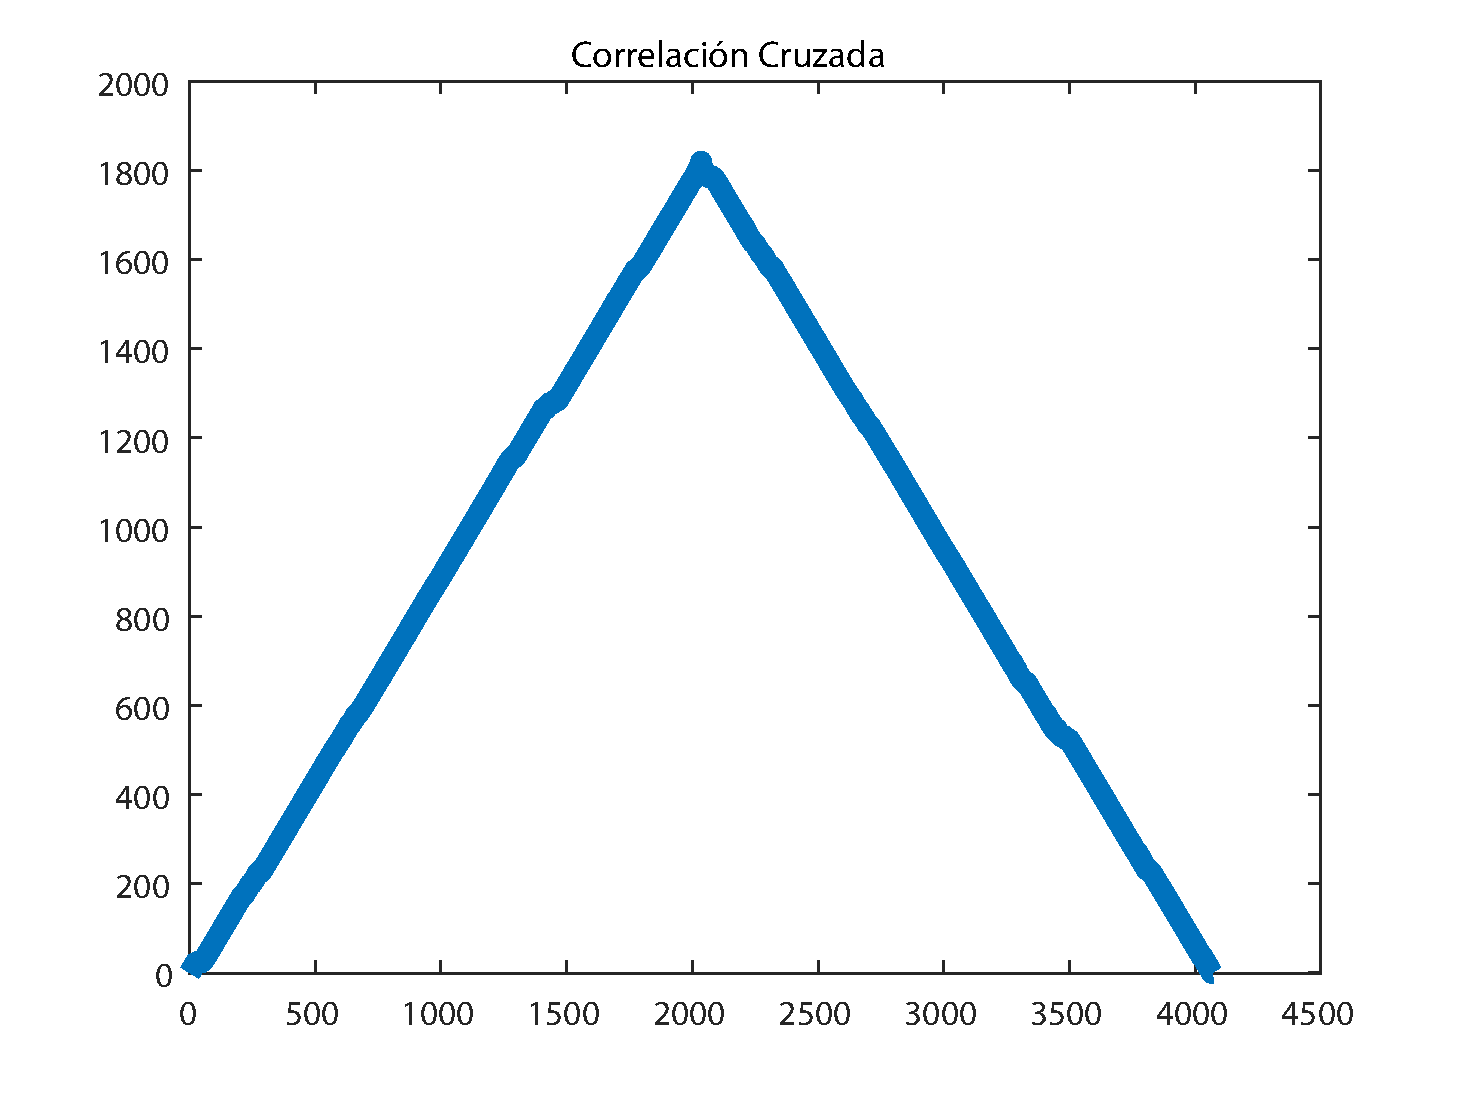
\includegraphics[scale=0.6]{./Figures/xcorrANN}
	\caption{Correlación cruzada entre modelos}
	\label{fig:xcorr}
\end{figure}

Con estos datos, es posible determinar que la implementación en Hardware es correcta y que funcionalmente se encuentra en capacidad de detectar eficazmente la probabilidad de inundación en comparación con un modelo netamente Software como el propuesto usando las herramientas de Matlab.

Es importante mencionar que el rendimiento de ambas redes, tanto la propuesta usando Matlab, como la desarrollada en Hardware dependende directamente de la calidad del entrenamiento y el set de datos elegido.
%Los resultados de detección para la red neuronal aquí expuestos implican que es posible usar configuraciones de redes neuronales mucho más complejas que en Matlab son muy simples de configurar y que los resultados del entrenamiento puedan ser llevados a la implementación Hardware sin dudas que la variación en la detección cambie drásticamente sin necesidad de implementar complejos algoritmos de entrenamiento usando C/C++ directamente sobre el hardware como aquí se propuso. % Diseño Experimental

% Chapter 12

\chapter{Análisis de Resultados} % Write in your own chapter title
\label{Chapter12}
\lhead{Capítulo 12. \emph{Resultados}} % Write in your own chapter title to set the page header

En este capítulo se muestran los resultados obtenidos en la implementación del hardware. Para esto se siguió la metodología descrita en el capítulo \ref{Chapter10}: 
 
 \section{Benchmark}
Dada la necesidad de medir el rendimiento del circuito implementado en HW contra la versión SW, se determinó que la mejor métrica se obtendría realizando un Benchmark de tres etapas con ejecuciones de 100 (\textbf{SW\_ 100M}) y 300 millones de operaciones por ejecución (\textbf{SW\_ 300M}), con la implementación en HW funcionando a 100MHz (\textbf{HW\_ 100M\_ 100MHz}, \textbf{HW\_ 300M\_ 100MHz}) y 150MHz (\textbf{HW\_ 100M\_ 150MHz}, \textbf{HW\_ 300M\_ 150MHz}), que son las frecuencias de reloj recomendadas por el sintetizador de alto nivel. La prueba consiste en cargar las neuronas de entrada y calcular el el tiempo que le tomó a ambas aproximaciones realizar el cálculo del resultado.

Como se observa en la Figura \ref{fig:benchmark}, las implementaciones \textbf{HW\_ 100M\_ 100MHz}, \textbf{HW\_ 100M\_ 150MHz}, \textbf{HW\_ 300M\_ 100MHz} y \textbf{HW\_ 300M\_ 150MHz} comparado con las implementaciones \textbf{SW\_ 100M} y \textbf{SW\_ 300M} la aceleración es aproximadamente cuatro veces. Esta prueba lo que busca es saturar el bus AMBA cargando y exigiendo al máximo el pipeline del bus usando las optimizaciones burst de la interfaz AXI. A diferencia de la implementación HW, la implementación software realiza una carga de las neuronas de entrada de forma secuencial adicionando un tiempo de carga alto debido a los múltiples llamados al bus que se encarga de la RAM.

%tek Revisar los valores numéricos

 \begin{figure}[!ht]
	\centering
		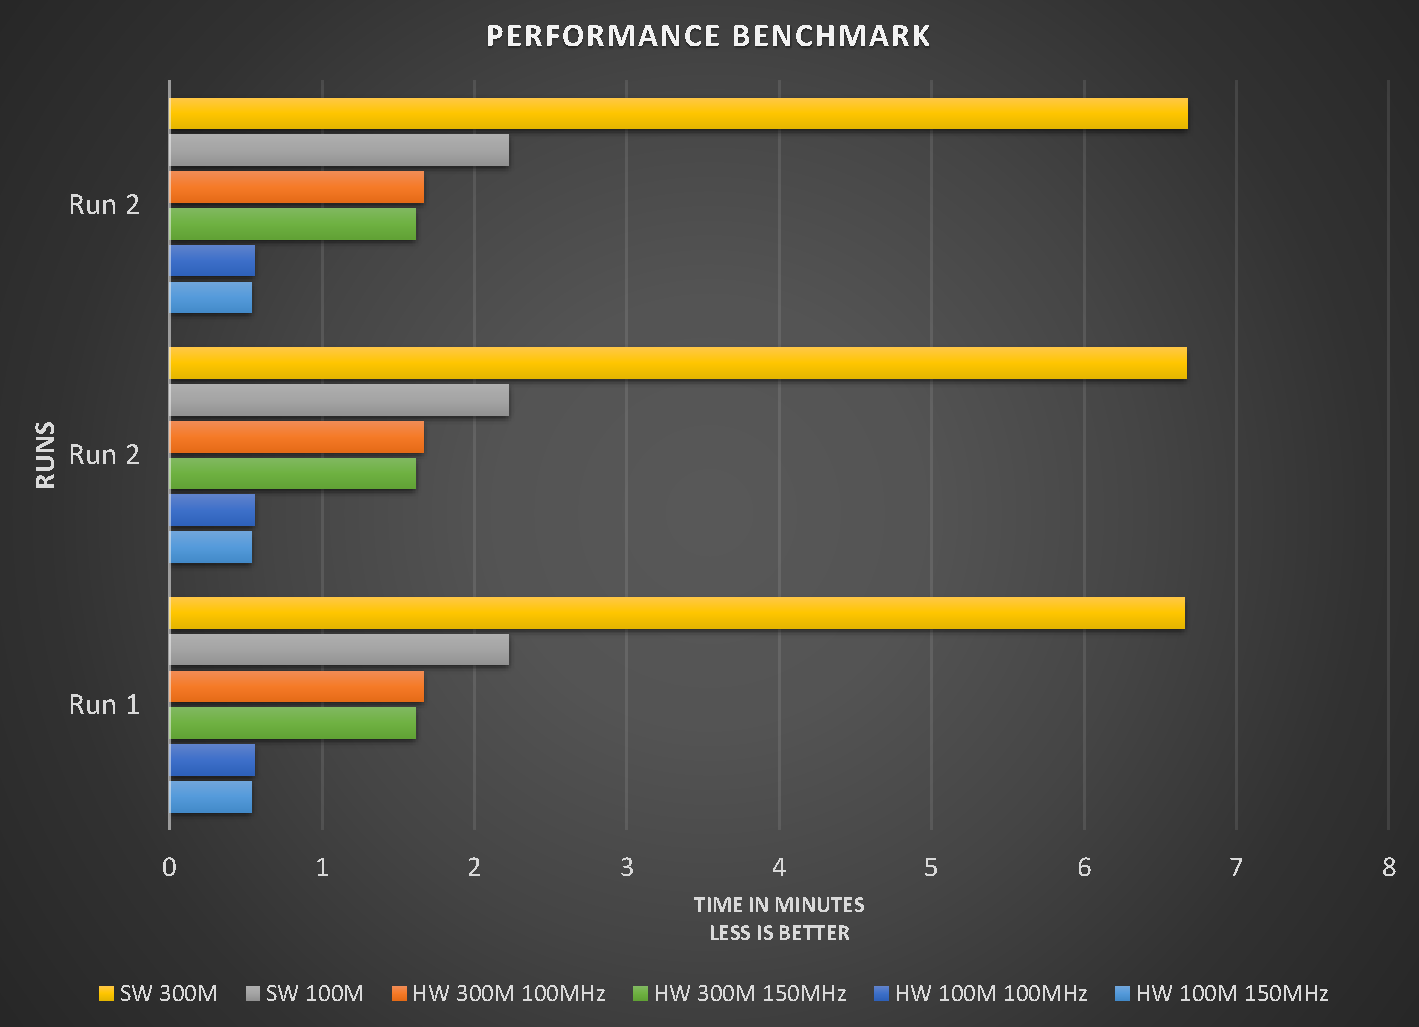
\includegraphics[scale=0.6]{Figures/performanceBenchmark}
	\caption{Benchmark resultados de la implementación}
	\label{fig:benchmark}
\end{figure}


\clearpage

\section{Análisis de tiempo y recursos}
\subsection{Tiempo de ejecución}

En la Figura \ref{fig:generalPerformance} se observan los resultados de la implementación de diferentes estrategias de optimización del hardware; en este caso tenemos: 
\begin{itemize}

\item WO-OPT: Sin optimizaciones.

\item P-UNROLL: Pipelining a nivel de bucles combinado con Unroll a los bucles.

\item DATAFLOW: Pipelining a nivel de tareas.

\item AO: Optimización de área.

\item PO: Pipelining a nivel de tareas, bucles y unroll

\end{itemize}

 \begin{figure}[!ht]
	\centering
		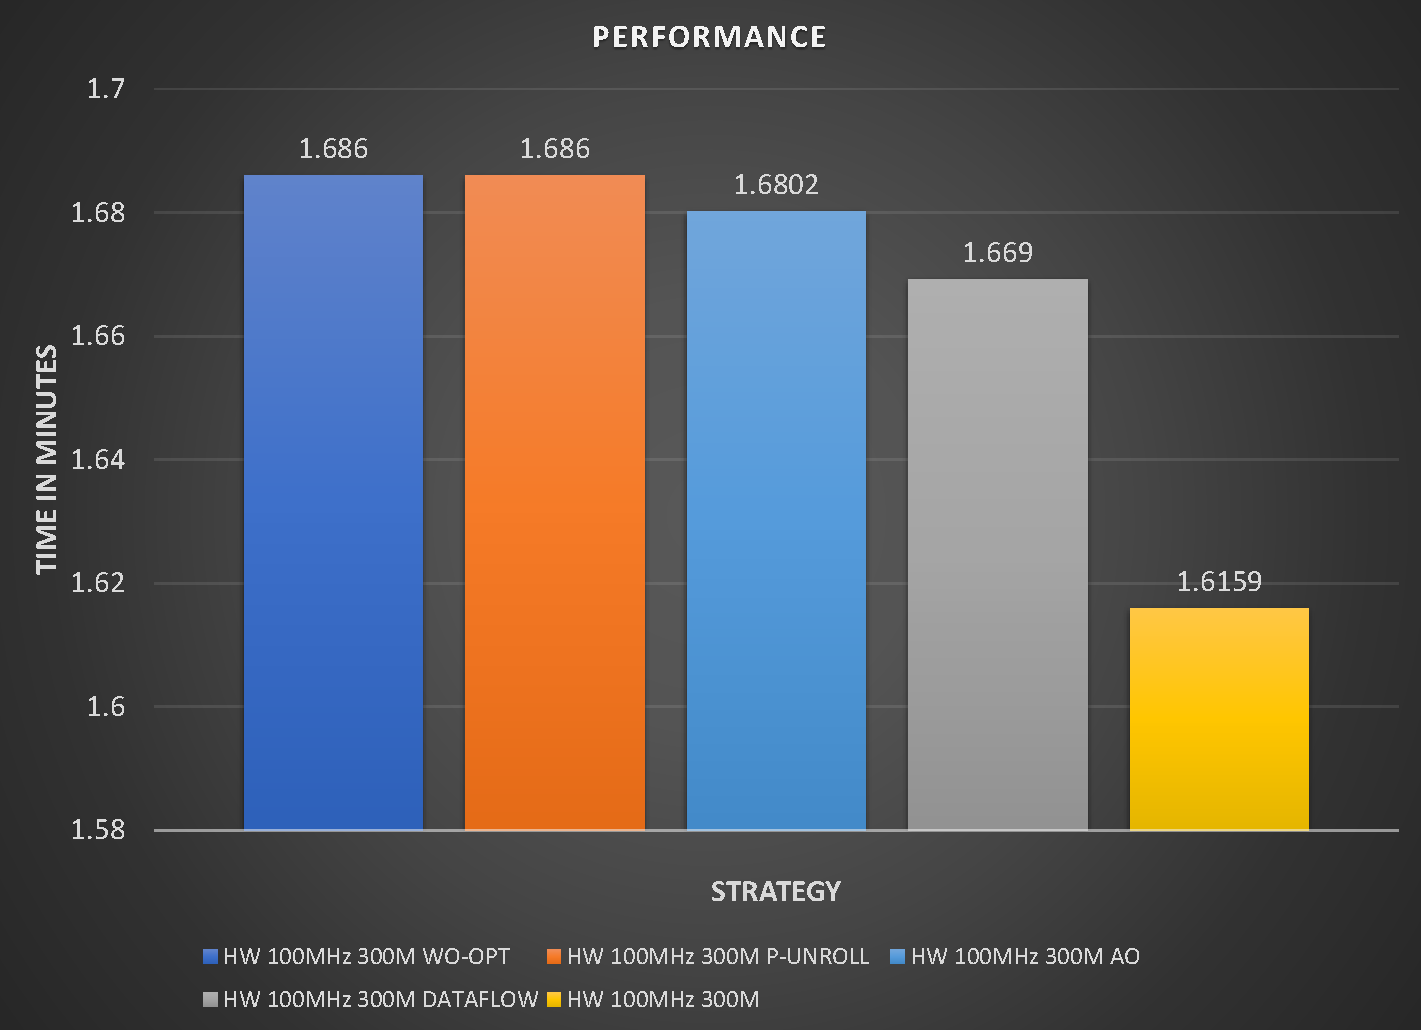
\includegraphics[scale=0.6]{Figures/generalPerformance}
	\caption{Rendimiento del acelerador en Hardware}
	\label{fig:generalPerformance}
\end{figure}

La Figura muestra claramente que la estrategia ``PO'' ofrece el mejor rendimiento en tiempo de ejecución de las tareas, siendo la estrategia a implementar en producción.

\clearpage

\subsection{Recursos utilizados}
Una vez determinados los tiempos de ejecución, se hace necesario tener en cuenta el área o la cantidad de recursos necesarios para cumplir las diferentes tareas de la solución. En este caso se analizó la cantidad de recursos para cada estrategia teniendo en cuenta el reporte del sintetizador de hardware Vivado.

La Figura \ref{fig:usedResources} muestra el porcentaje de recursos usados por cada una de las diferentes estrategias. Es importante notar que la estrategia ``AO'' usa 51\% menos LUT, 42\% menos DSPs y 37\% menos BRAM que su contraparte ``PO'' para un rendimiento casi marginal en tiempo.

\begin{figure}[!ht]
	\centering
		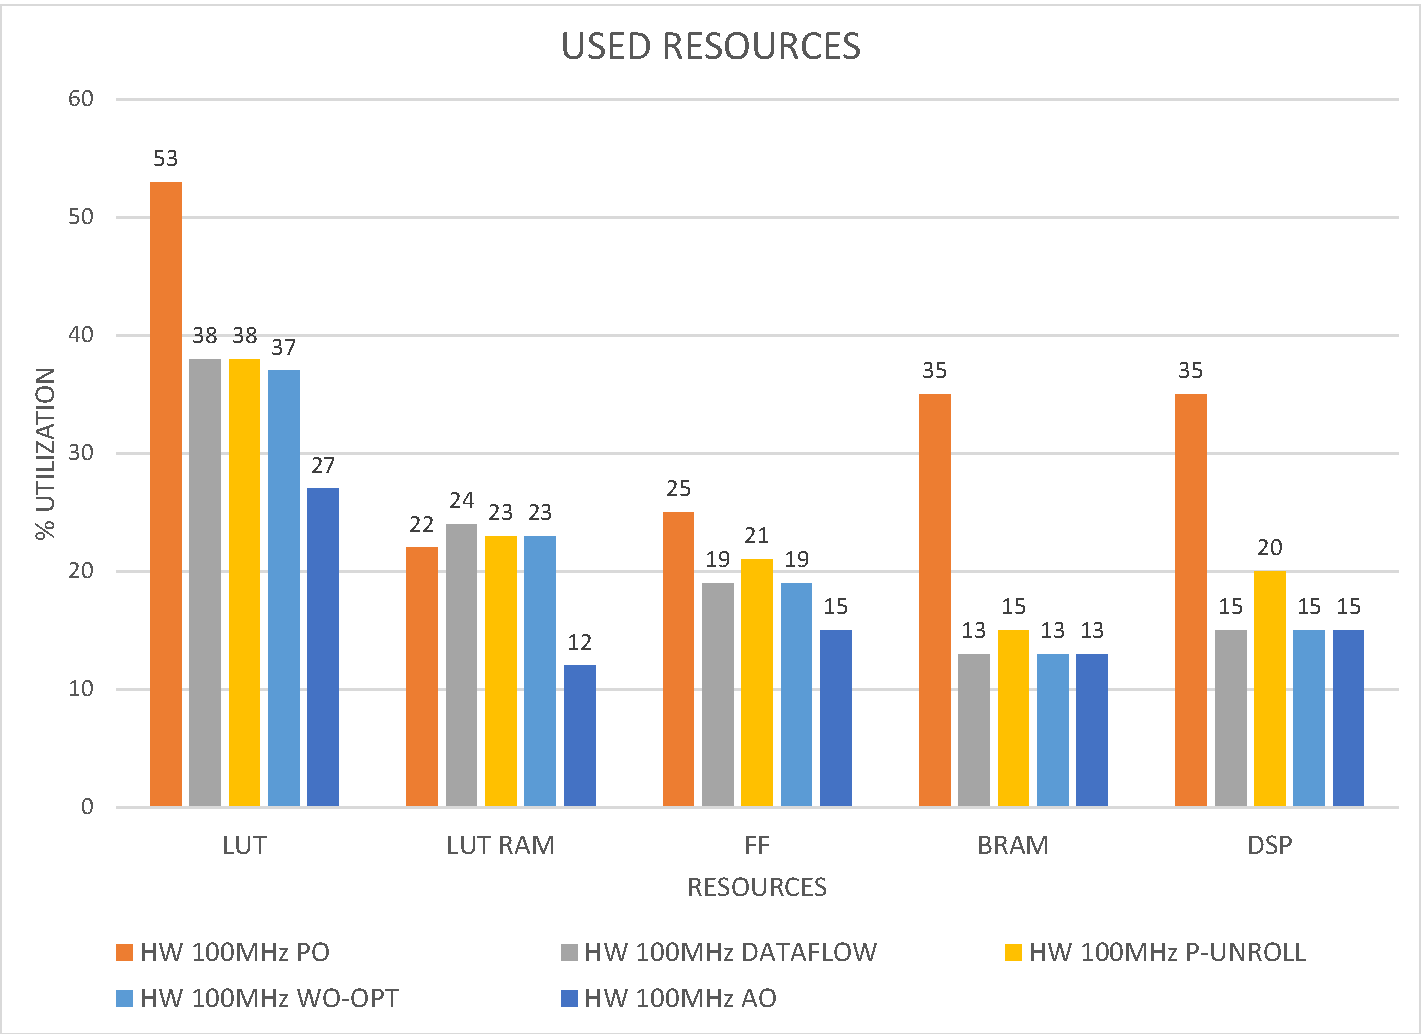
\includegraphics[scale=0.6]{Figures/usedResources}
	\caption{Recursos utilizados en la FPGA}
	\label{fig:usedResources}
\end{figure}

La Figura \ref{fig:performanceResources} muestra claramente que la estrategia ``AO'' es aproximadamente 46\% más eficiente que su contraparte ``PO''. De esta forma, es posible determinar que, al usar menos área vamos a obtener un mejor delta de eficiencia, pues al usar menos recursos es posible adicionar más módulos de hardware o, en otros casos, usar menos potencia en tiempo de ejecución.

\begin{figure}[!ht]
	\centering
		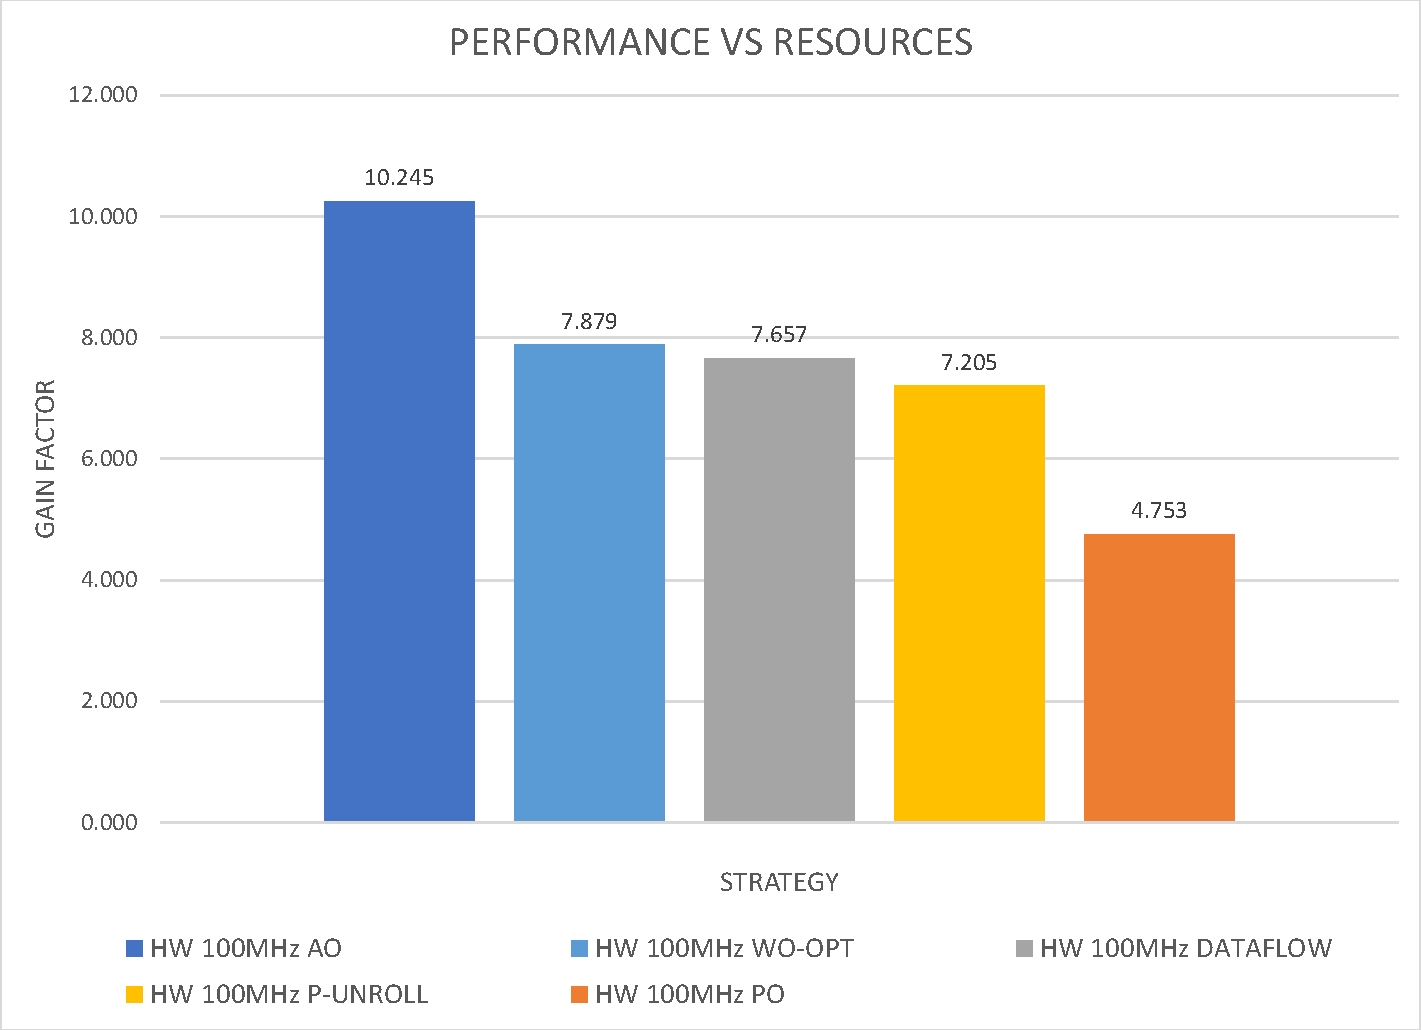
\includegraphics[scale=0.6]{Figures/performanceResources}
	\caption{Factor de ganancia recursos contra tiempo}
	\label{fig:performanceResources}
\end{figure}
 % Modelo ANN

% Chapter 13

\chapter{Análisis de Resultados} % Write in your own chapter title
\label{Chapter13}
\lhead{Capítulo 13. \emph{Resultados}} % Write in your own chapter title to set the page header

En este capítulo se muestran los resultados obtenidos en la implementación del hardware. Para esto se siguió la metodología descrita en el capítulo \ref{Chapter11}: 
 
 \section{Benchmark}
Dada la necesidad de medir el rendimiento del circuito implementado en HW contra la versión SW, se determinó que la mejor métrica se obtendría realizando un Benchmark de tres etapas con ejecuciones de 100 (\textbf{SW\_ 100M}) y 300 millones de operaciones por ejecución (\textbf{SW\_ 300M}), con la implementación en HW funcionando a 100MHz (\textbf{HW\_ 100M\_ 100MHz}, \textbf{HW\_ 300M\_ 100MHz}) y 150MHz (\textbf{HW\_ 100M\_ 150MHz}, \textbf{HW\_ 300M\_ 150MHz}), que son las frecuencias de reloj recomendadas por el sintetizador de alto nivel. La prueba consiste en cargar las neuronas de entrada y calcular el tiempo que le tomó a ambas aproximaciones realizar el cálculo del resultado.

Como se observa en la Figura \ref{fig:benchmark}, las implementaciones \textbf{HW\_ 100M\_ 100MHz}, \textbf{HW\_ 100M\_ 150MHz}, \textbf{HW\_ 300M\_ 100MHz} y \textbf{HW\_ 300M\_ 150MHz} comparado con las implementaciones \textbf{SW\_ 100M} y \textbf{SW\_ 300M} la aceleración es aproximadamente cuatro veces. Esta prueba lo que busca es saturar el bus AMBA cargando y exigiendo al máximo el pipeline del bus usando las optimizaciones burst de la interfaz AXI. A diferencia de la implementación HW, la implementación software realiza una carga de las neuronas de entrada de forma secuencial adicionando un tiempo de carga alto debido a los múltiples llamados al bus que se encarga de la RAM.

%tek Revisar los valores numéricos

 \begin{figure}[!ht]
	\centering
		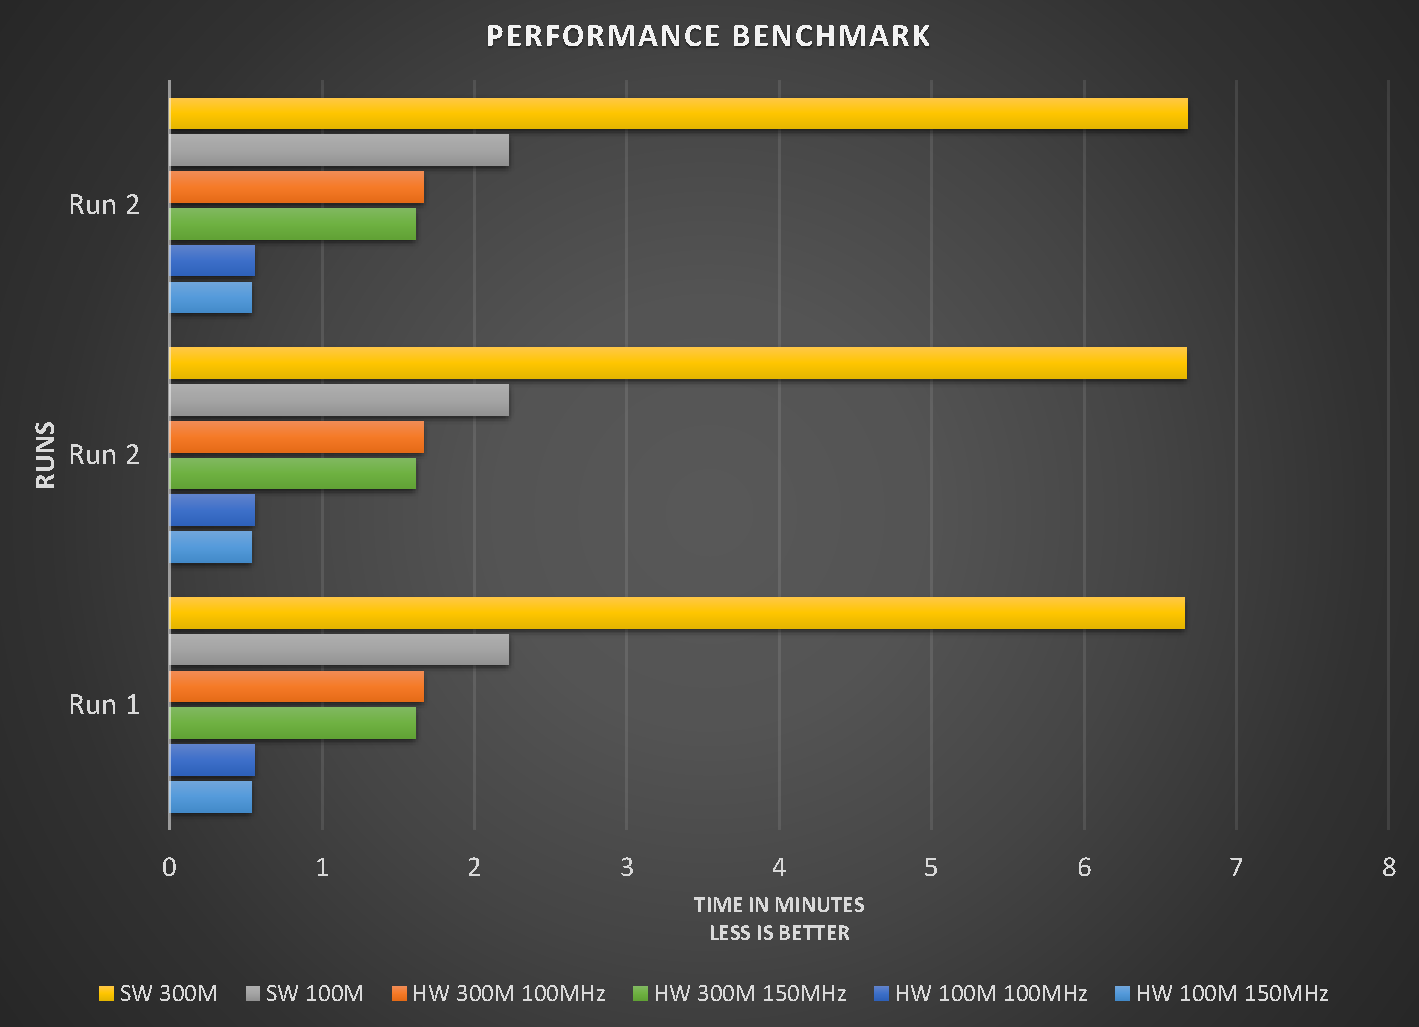
\includegraphics[scale=0.6]{Figures/performanceBenchmark}
	\caption{Benchmark resultados de la implementación}
	\label{fig:benchmark}
\end{figure}


\clearpage

\section{Análisis de tiempo y recursos}
\subsection{Tiempo de ejecución}

En la Figura \ref{fig:generalPerformance} se observan los resultados de la implementación de diferentes estrategias de optimización del hardware; en este caso tenemos: 
\begin{itemize}

\item WO-OPT: Sin optimizaciones.

\item P-UNROLL: Pipelining a nivel de bucles combinado con Unroll a los bucles.

\item DATAFLOW: Pipelining a nivel de tareas.

\item AO: Optimización de área.

\item PO: Pipelining a nivel de tareas, bucles y unroll

\end{itemize}

 \begin{figure}[!ht]
	\centering
		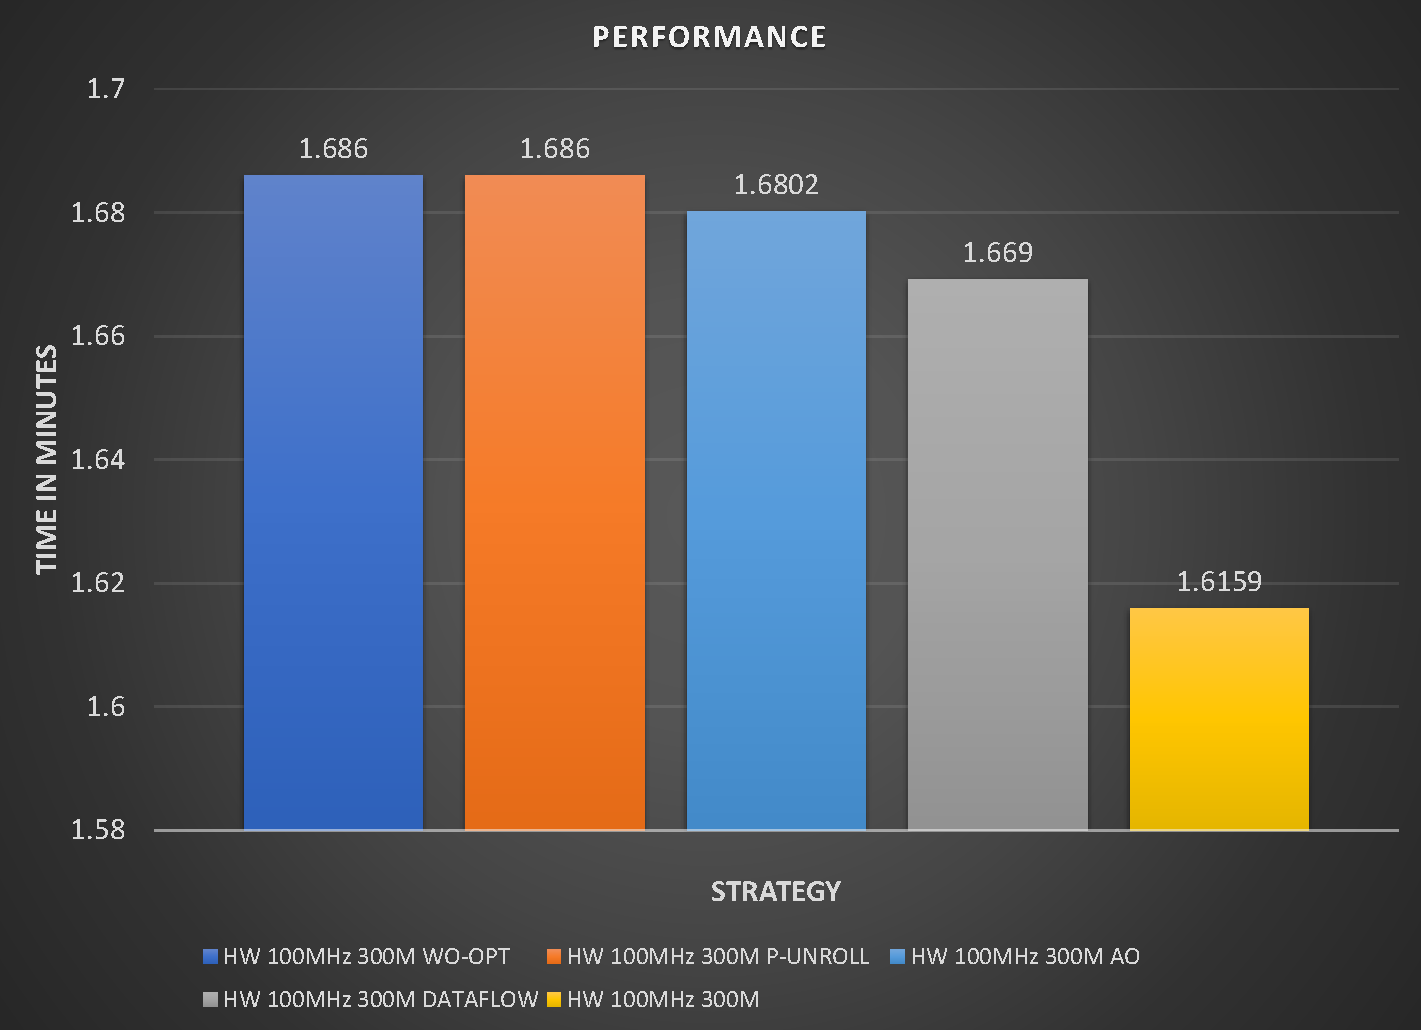
\includegraphics[scale=0.6]{Figures/generalPerformance}
	\caption{Rendimiento del acelerador en Hardware}
	\label{fig:generalPerformance}
\end{figure}

La Figura muestra claramente que la estrategia ``PO'' ofrece el mejor rendimiento en tiempo de ejecución de las tareas, siendo la estrategia a implementar en producción.

\clearpage

\subsection{Recursos utilizados}
Una vez determinados los tiempos de ejecución, se hace necesario tener en cuenta el área o la cantidad de recursos necesarios para cumplir las diferentes tareas de la solución. En este caso se analizó la cantidad de recursos para cada estrategia teniendo en cuenta el reporte del sintetizador de hardware Vivado.

La Figura \ref{fig:usedResources} muestra el porcentaje de recursos usados por cada una de las diferentes estrategias. Es importante notar que la estrategia ``AO'' usa 51\% menos LUT, 42\% menos DSPs y 37\% menos BRAM que su contraparte ``PO'' para un rendimiento casi marginal en tiempo.

\begin{figure}[!ht]
	\centering
		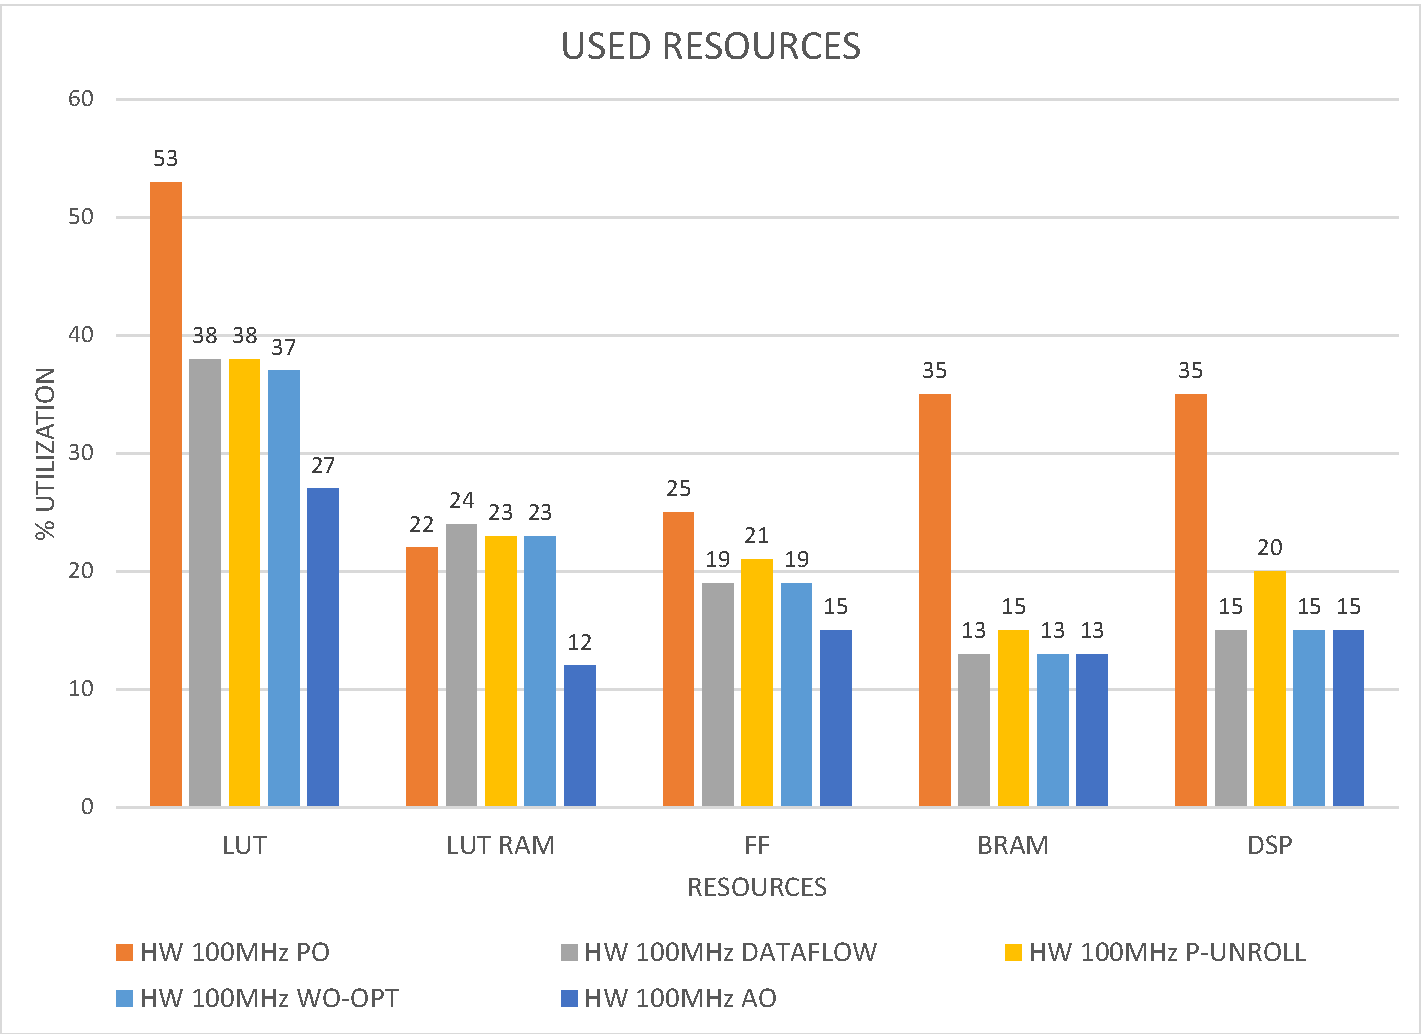
\includegraphics[scale=0.6]{Figures/usedResources}
	\caption{Recursos utilizados en la FPGA}
	\label{fig:usedResources}
\end{figure}

La Figura \ref{fig:performanceResources} muestra claramente que la estrategia ``AO'' es aproximadamente 46\% más eficiente que su contraparte ``PO''. De esta forma, es posible determinar que, al usar menos área vamos a obtener un mejor delta de eficiencia, pues al usar menos recursos es posible adicionar más módulos de hardware o, en otros casos, usar menos potencia en tiempo de ejecución.

\begin{figure}[!ht]
	\centering
		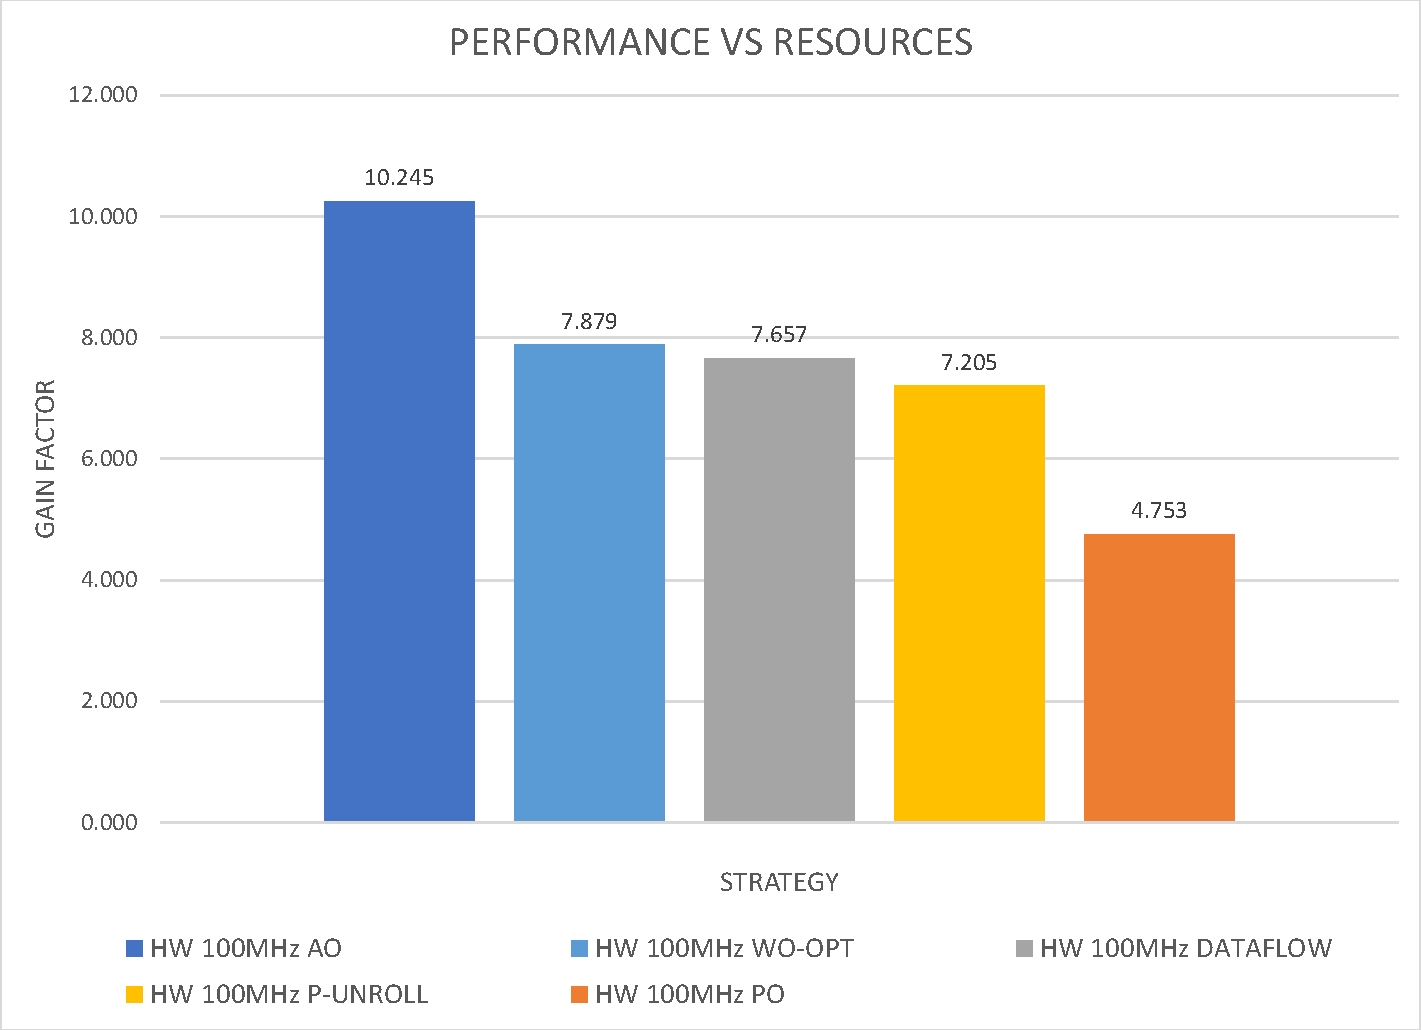
\includegraphics[scale=0.6]{Figures/performanceResources}
	\caption{Factor de ganancia recursos contra tiempo}
	\label{fig:performanceResources}
\end{figure}
 % Comparación Modelo ANN

% Chapter 14

\chapter{Análisis de Resultados} % Write in your own chapter title
\label{Chapter14}
\lhead{Capítulo 14. \emph{Resultados}} % Write in your own chapter title to set the page header

En este capítulo se muestran los resultados obtenidos en la implementación del hardware. Para esto se siguió la metodología descrita en el capítulo \ref{Chapter11}: 
 
 \section{Benchmark}
Dada la necesidad de medir el rendimiento del circuito implementado en HW contra la versión SW, se determinó que la mejor métrica se obtendría realizando un Benchmark de tres etapas con ejecuciones de 100 (\textbf{SW\_ 100M}) y 300 millones de operaciones por ejecución (\textbf{SW\_ 300M}), con la implementación en HW funcionando a 100MHz (\textbf{HW\_ 100M\_ 100MHz}, \textbf{HW\_ 300M\_ 100MHz}) y 150MHz (\textbf{HW\_ 100M\_ 150MHz}, \textbf{HW\_ 300M\_ 150MHz}), que son las frecuencias de reloj recomendadas por el sintetizador de alto nivel. La prueba consiste en cargar las neuronas de entrada y calcular el tiempo que le tomó a ambas aproximaciones realizar el cálculo del resultado.

Como se observa en la Figura \ref{fig:benchmark}, las implementaciones \textbf{HW\_ 100M\_ 100MHz}, \textbf{HW\_ 100M\_ 150MHz}, \textbf{HW\_ 300M\_ 100MHz} y \textbf{HW\_ 300M\_ 150MHz} comparado con las implementaciones \textbf{SW\_ 100M} y \textbf{SW\_ 300M} la aceleración es aproximadamente cuatro veces. Esta prueba lo que busca es saturar el bus AMBA cargando y exigiendo al máximo el pipeline del bus usando las optimizaciones burst de la interfaz AXI. A diferencia de la implementación HW, la implementación software realiza una carga de las neuronas de entrada de forma secuencial adicionando un tiempo de carga alto debido a los múltiples llamados al bus que se encarga de la RAM.

%tek Revisar los valores numéricos

 \begin{figure}[!ht]
	\centering
		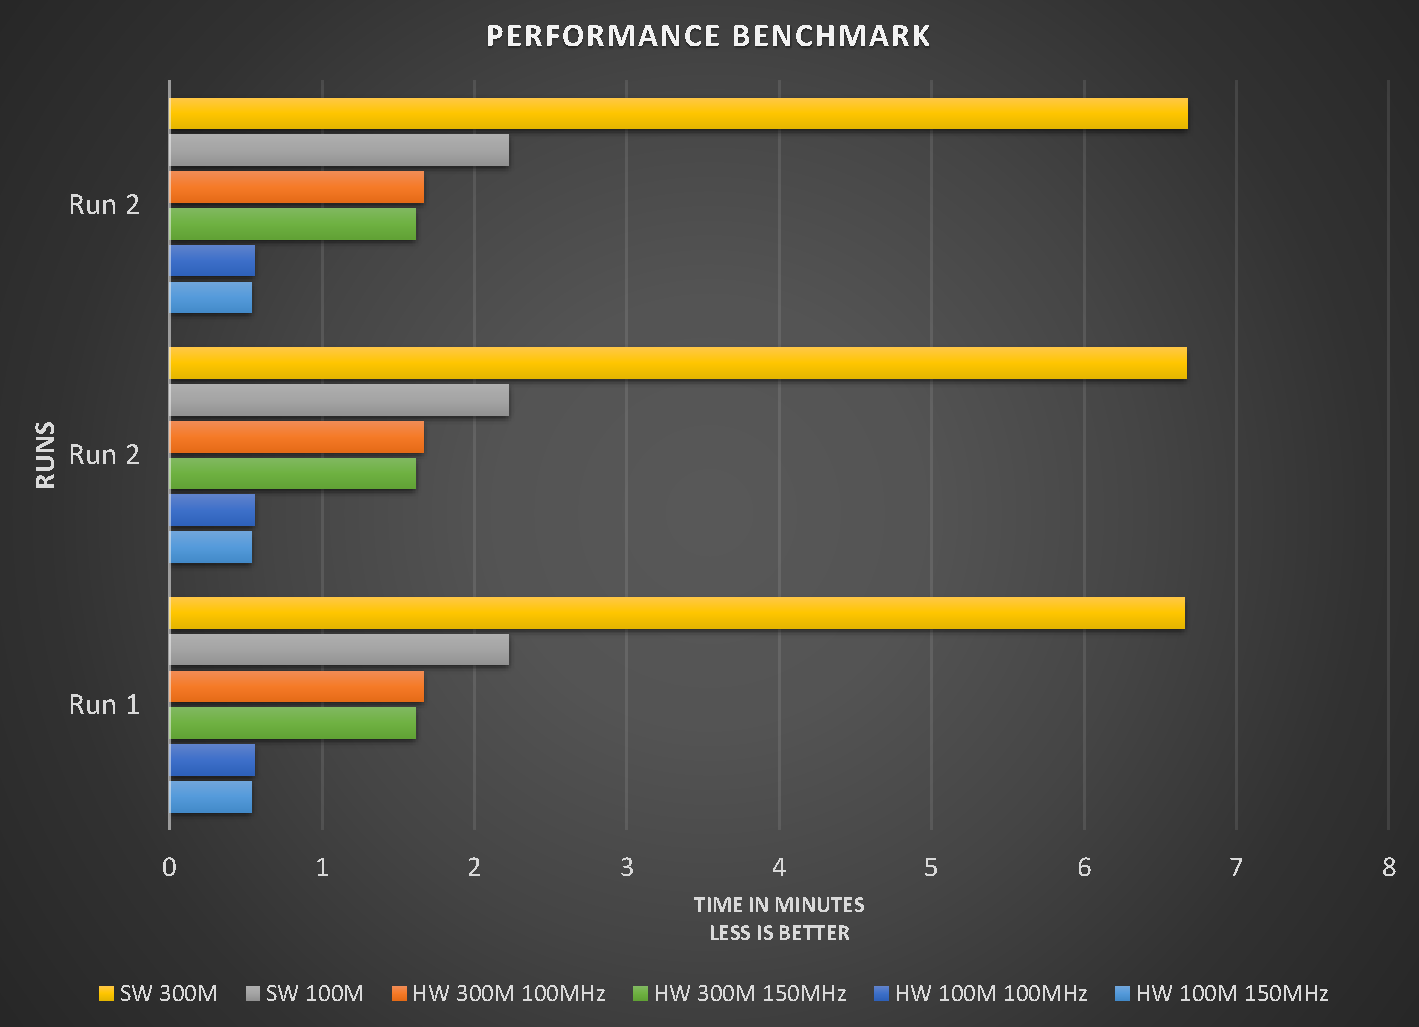
\includegraphics[scale=0.6]{Figures/performanceBenchmark}
	\caption{Benchmark resultados de la implementación}
	\label{fig:benchmark}
\end{figure}


\clearpage

\section{Análisis de tiempo y recursos}
\subsection{Tiempo de ejecución}

En la Figura \ref{fig:generalPerformance} se observan los resultados de la implementación de diferentes estrategias de optimización del hardware; en este caso tenemos: 
\begin{itemize}

\item WO-OPT: Sin optimizaciones.

\item P-UNROLL: Pipelining a nivel de bucles combinado con Unroll a los bucles.

\item DATAFLOW: Pipelining a nivel de tareas.

\item AO: Optimización de área.

\item PO: Pipelining a nivel de tareas, bucles y unroll

\end{itemize}

 \begin{figure}[!ht]
	\centering
		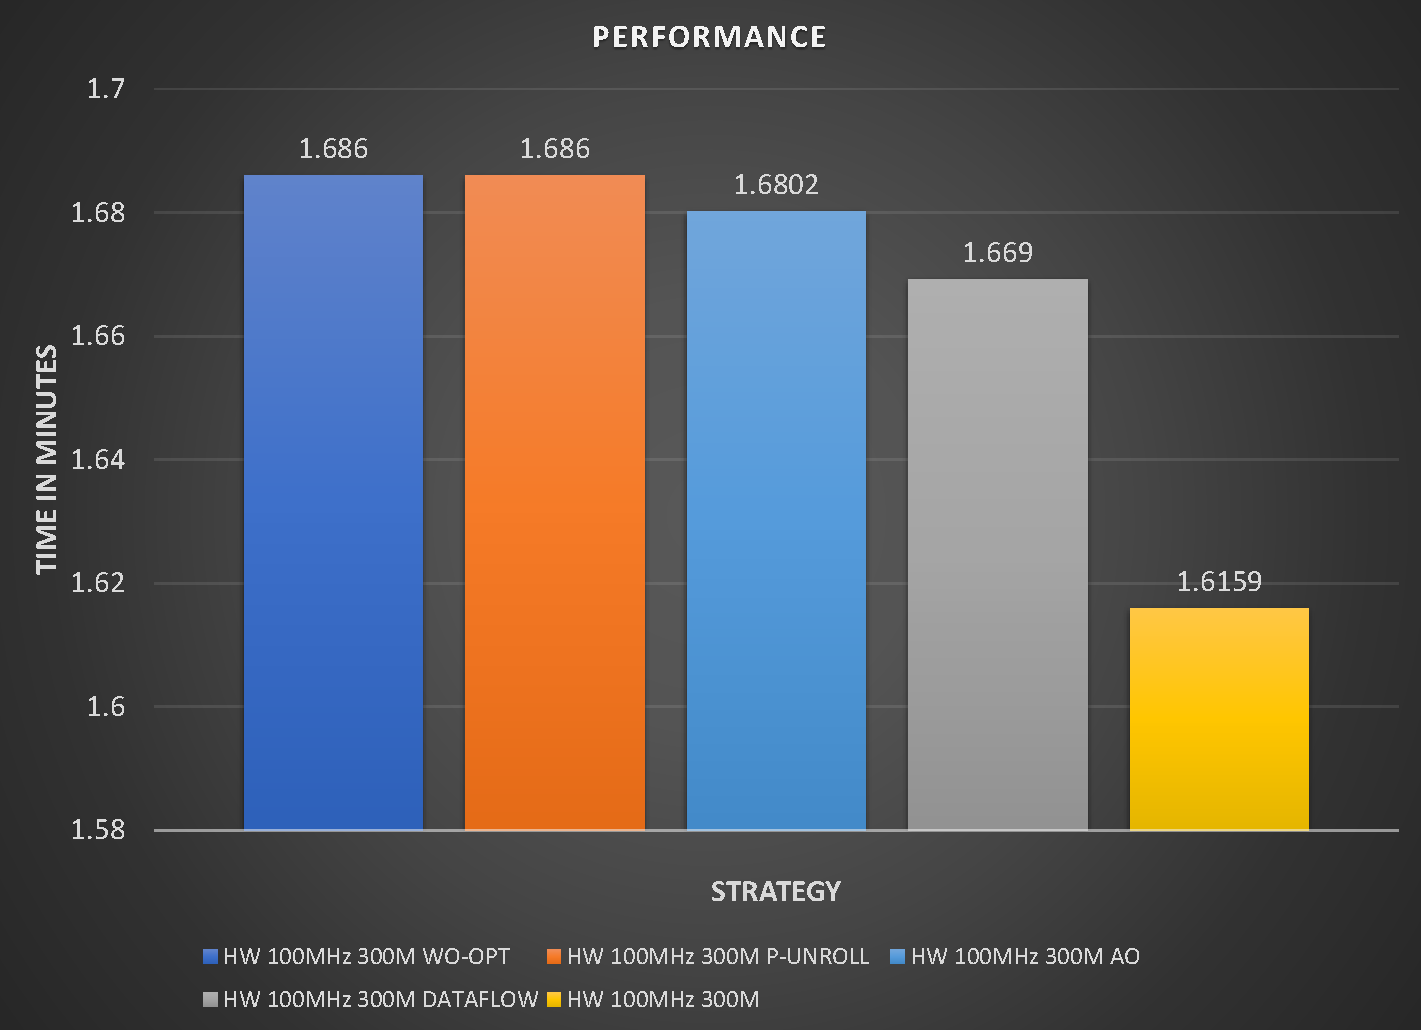
\includegraphics[scale=0.6]{Figures/generalPerformance}
	\caption{Rendimiento del acelerador en Hardware}
	\label{fig:generalPerformance}
\end{figure}

La Figura muestra claramente que la estrategia ``PO'' ofrece el mejor rendimiento en tiempo de ejecución de las tareas, siendo la estrategia a implementar en producción.

\clearpage

\subsection{Recursos utilizados}
Una vez determinados los tiempos de ejecución, se hace necesario tener en cuenta el área o la cantidad de recursos necesarios para cumplir las diferentes tareas de la solución. En este caso se analizó la cantidad de recursos para cada estrategia teniendo en cuenta el reporte del sintetizador de hardware Vivado.

La Figura \ref{fig:usedResources} muestra el porcentaje de recursos usados por cada una de las diferentes estrategias. Es importante notar que la estrategia ``AO'' usa 51\% menos LUT, 42\% menos DSPs y 37\% menos BRAM que su contraparte ``PO'' para un rendimiento casi marginal en tiempo.

\begin{figure}[!ht]
	\centering
		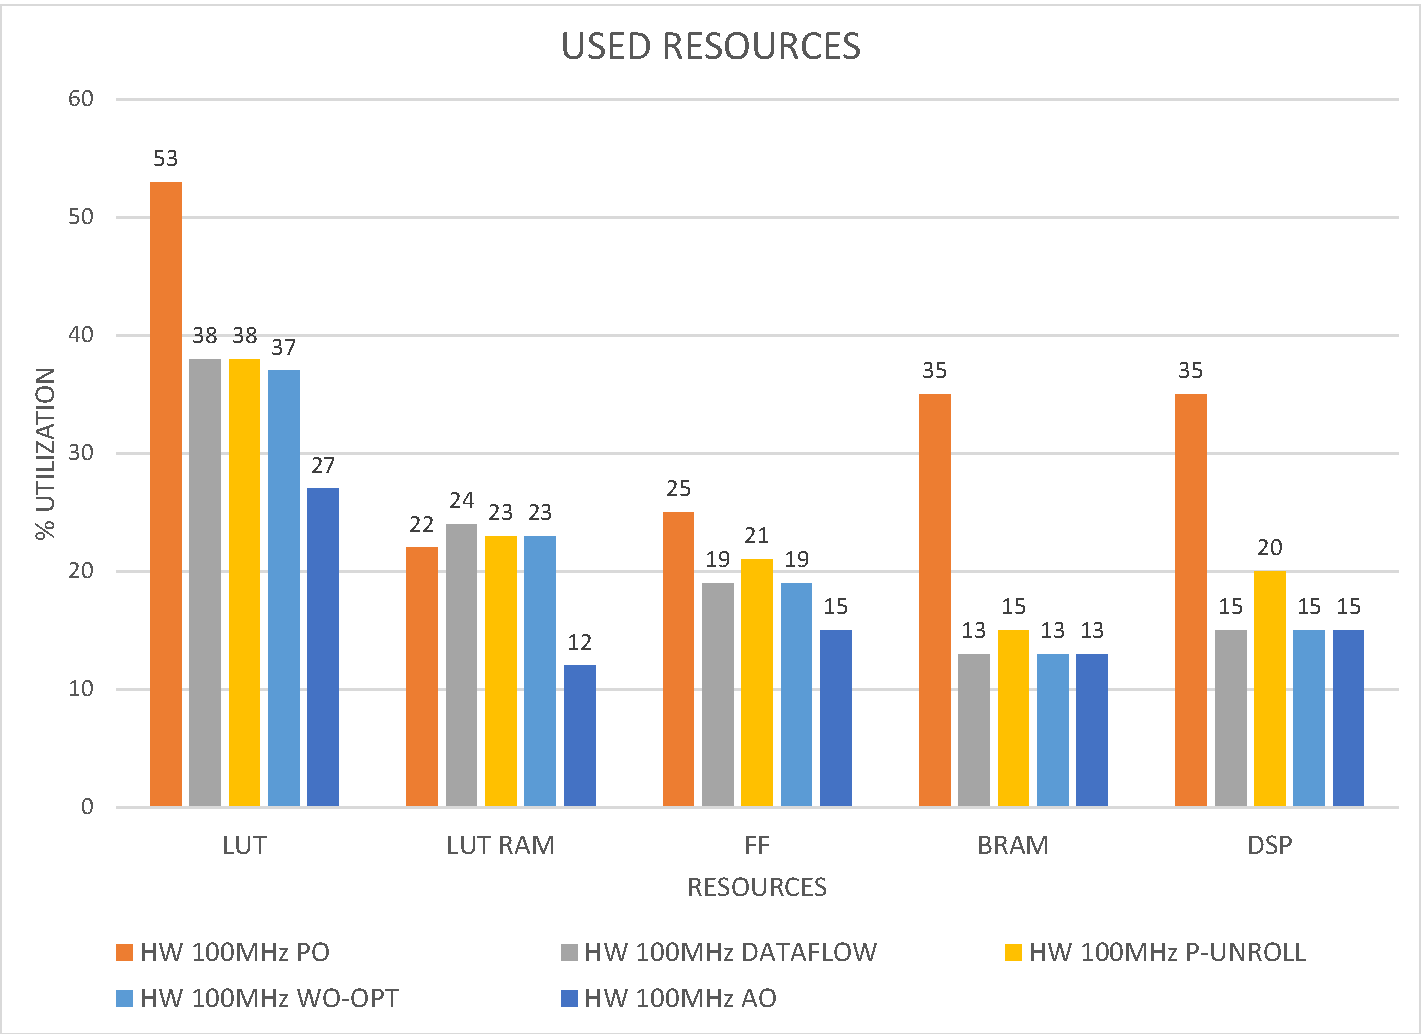
\includegraphics[scale=0.6]{Figures/usedResources}
	\caption{Recursos utilizados en la FPGA}
	\label{fig:usedResources}
\end{figure}

La Figura \ref{fig:performanceResources} muestra claramente que la estrategia ``AO'' es aproximadamente 46\% más eficiente que su contraparte ``PO''. De esta forma, es posible determinar que, al usar menos área vamos a obtener un mejor delta de eficiencia, pues al usar menos recursos es posible adicionar más módulos de hardware o, en otros casos, usar menos potencia en tiempo de ejecución.

\begin{figure}[!ht]
	\centering
		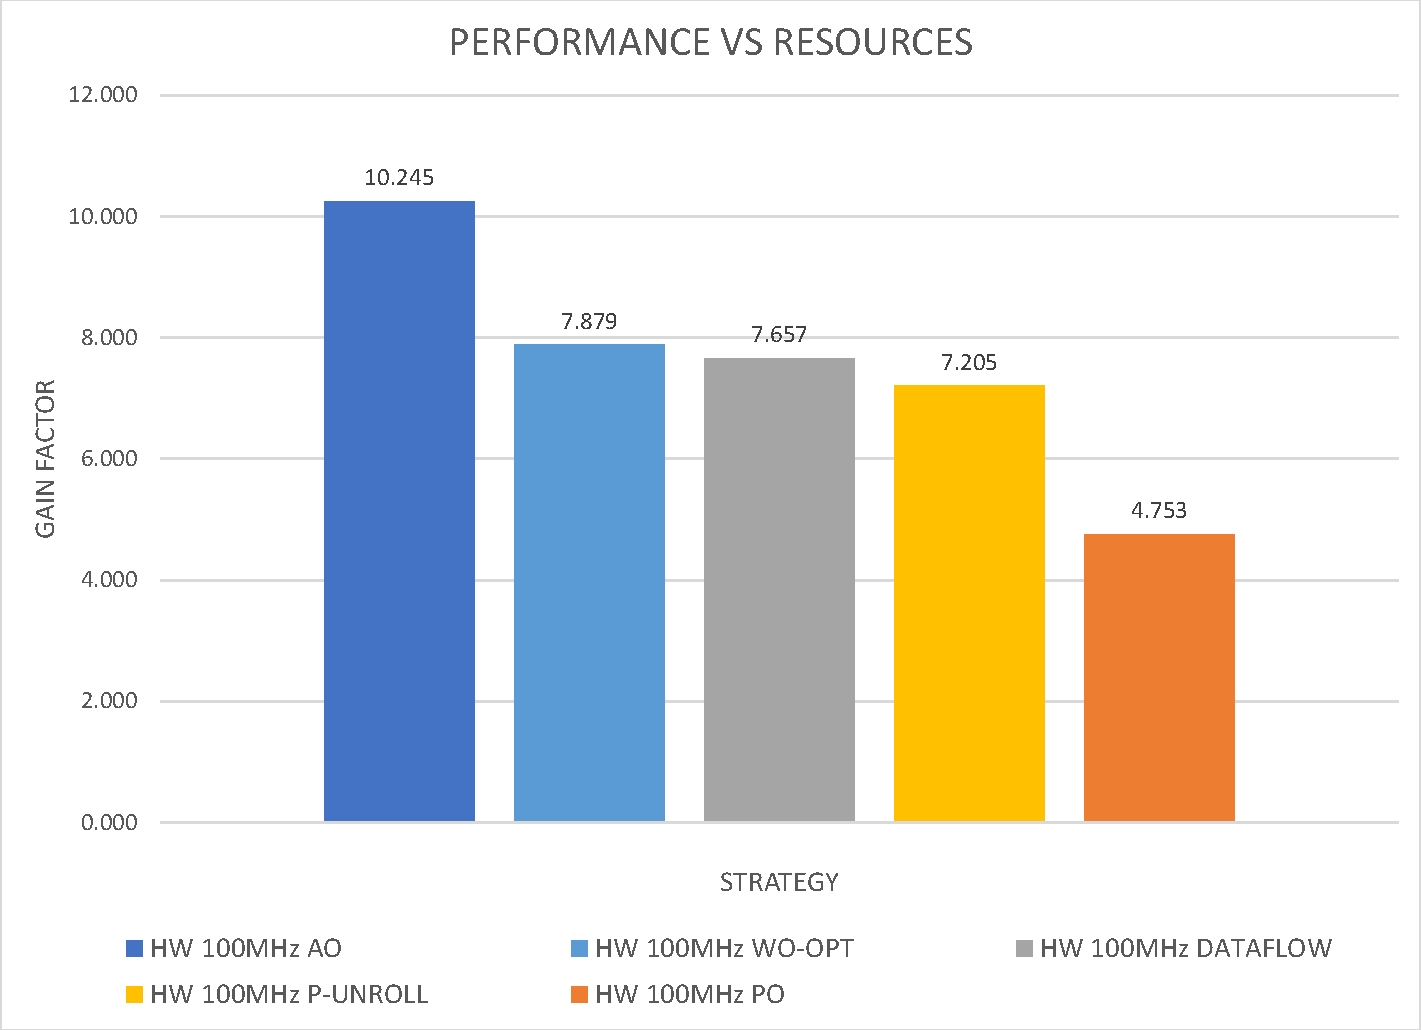
\includegraphics[scale=0.6]{Figures/performanceResources}
	\caption{Factor de ganancia recursos contra tiempo}
	\label{fig:performanceResources}
\end{figure}
 % Resultados

% Chapter 15

\chapter{Conclusiones} % Write in your own chapter title
\label{Chapter15}
\lhead{Capítulo 15. \emph{Conclusiones}} % Write in your own chapter title to set the page header

De acuerdo con la revisión del estado del arte no se encontró una solución que articule las dimensiones de aceleración y reconfiguración dinámica del hardware en una plataforma de computación de borde usando un esquema orientado al Internet de las Cosas, por lo cual se considera que el enfoque que se plantea en este trabajo es la principal contribución del mismo.

En particular, se muestra que el procesamiento y fusión de altos volúmenes de datos en el borde de una red IoT es posible usando dispositivos orientados al Internet de las Cosas con hardware para incrementar la potencia de cálculo y software especializado para coordinar y adicionar funcionalidad basado en esquemas de reconfiguración dinámica del hardware. Con un diseño de hardware y las optimizaciones propuestas, es posible realizar múltiples operaciones sobre los datos concurrentemente con un bajo footprint sobre el procesador, relegando únicamente la carga operativa a la FPGA y dejando que el procesador atienda los diferentes servicios de red que implican una conexión con la Nube.

La elección del hardware y los recursos necesarios para la implementación de una plataforma de computación de borde están basados netamente en las necesidades que se desean cumplir. En este caso, hay indicios de que con un hardware (procesador, memoria, almacenamiento) relativamente limitado es posible prototipar y posteriormente desplegar en producción un dispositivo enteramente capaz de realizar el trabajo de otros dispositivos con TDP mucho más altos. 

Se determinó que es posible implementar directamente el modelo Hardware entrenado, garantizando el funcionamiento y detección basado en un modelo software usando las herramientas de desarrollo y entrenamiento de Matlab.

Más aún, una implementación directamente sobre el hardware permite tener control fino sobre las diferentes etapas de optimización, manipulación de los datos y consumo de recursos de hardware a diferencia de implementaciones usando las herramientas de Matlab como System Generator que permiten sintetizar hardware a un nivel muy alto sin opciones de optimización y consumo de recursos para sistemas como el propuesto en el que el hardware es muy limitado.

Como parte de la funcionalidad de la plataforma, se integraron exitosamente los múltiples módulos de hardware como bloques IP en forma de repositorio; estos se encuentran almacenados al interior de la memoria micro SD que contiene el File System y la configuración de arranque del sistema operativo. Esto con el objetivo de que la plataforma de computación de borde tenga a disposición local los módulos que permitan la reconfiguración de la FPGA en tiempo de ejecución.

El diseño de hardware propuesto proporciona una ganancia de 4x la velocidad de cálculo sobre su contraparte software con el mismo diseño base, convirtiéndolo en una solución mucho más eficiente para el procesamiento de los datos en el borde de una red IoT. Además, con las optimizaciones de área correctas es posible integrar múltiples módulos IP que realicen diferentes operaciones y transformaciones sobre los datos, sacrificando rendimiento que puede o no ser notable, dependiendo de la complejidad y optimizaciones de hardware que requiera el circuito.

La implementación de una solución como la propuesta requiere de pasos muy precisos en la configuración del kernel, más aún si se desean características especificas como un sistema de archivos de Ubuntu o módulos de hardware como una DMA para video o para mover grandes bloques de datos de una región a otra de memoria. Con una arquitectura como la propuesta es posible configurar la FPGA en tiempo de ejecución del Kernel de Linux y adicionar nuevos binarios y configuraciones al sistema de archivos usando un servidor sftp y un cliente como FileZilla.

Se estableció que el ancho en bits del bus de datos del circuito hardware no influye sobre la latencia total del circuito, con lo cual se pudo implementar un ancho de datos de 32 bits, garantizando así una alta resolución para las operaciones sin perder rendimiento.

Durante la etapa de desarrollo inicial del hardware se determinó que el canal de datos de alta velocidad ofrecido por la interfaz AXI Full es el requerido para una aplicación donde el alto volumen de datos a procesar es un factor determinante para el rendimiento total de la solución. Esto se evidencia al implementar la solución con la interfaz AXI Lite, con la cual se obtuvo un rendimiento más bajo que la solución netamente software. % Conclusiones


%% ----------------------------------------------------------------
% Now begin the Appendices, including them as separate files

\addtocontents{toc}{\vspace{2em}} % Add a gap in the Contents, for aesthetics

\appendix % Cue to tell LaTeX that the following 'chapters' are Appendices

%\input{./Appendices/AppendixA}	% Appendix Title

%\input{./Appendices/AppendixB} % Appendix Title

%\input{./Appendices/AppendixC} % Appendix Title

%% ----------------------------------------------------------------
\addtocontents{toc}{\vspace{2em}}  % Add a gap in the Contents, for aesthetics
\backmatter
%% ----------------------------------------------------------------
\label{Bibliography}

\lhead{\emph{Bibliography}}  % Change the left side page header to "Bibliography"
%\bibliographystyle{unsrtnat}  % Use the "unsrtnat" BibTeX style for formatting the Bibliography
\bibliographystyle{ieeetr}
\bibliography{Bibliography}  % The references (bibliography) information are stored in the file named "Bibliography.bib"
\end{document}  % The End
%% ----------------------------------------------------------------